%==================================================================================
%==================================================================================
\documentclass[11pt]{beamer}
%==================================================================================
%==================================================================================
\mode<presentation>
{
  \usetheme{default}      % or try Darmstadt, Madrid, Warsaw, ...
  \usecolortheme{default} % or try albatross, beaver, crane, ...
  \usefonttheme{default}  % or try serif, structurebold, ...
  \setbeamertemplate{navigation symbols}{}
  \setbeamertemplate{caption}[numbered]
  \setbeamertemplate{footline}[frame number]
  \setbeamerfont{frametitle}{size=\large,series=\bfseries}
  \setbeamercolor{frametitle}{fg=blue}
  \setbeamercolor{background canvas}{bg=white}
  \setbeamercolor{normal text}{fg=black}
}

%==================================================================================

\usepackage[english]{babel}
\usepackage[utf8x]{inputenc}
\usepackage{graphicx}
\usepackage{hyperref}
\definecolor{snow}{rgb}{1.000,0.980,0.980}
\definecolor{snow1}{rgb}{1.000,0.980,0.980}
\definecolor{snow2}{rgb}{0.933,0.914,0.914}
\definecolor{snow3}{rgb}{0.804,0.788,0.788}
\definecolor{snow4}{rgb}{0.545,0.537,0.537}
\definecolor{GhostWhite}{rgb}{0.973,0.973,1.000}
\definecolor{WhiteSmoke}{rgb}{0.961,0.961,0.961}
\definecolor{gainsboro}{rgb}{0.863,0.863,0.863}
\definecolor{FloralWhite}{rgb}{1.000,0.980,0.941}
\definecolor{OldLace}{rgb}{0.992,0.961,0.902}
\definecolor{linen}{rgb}{0.980,0.941,0.902}
\definecolor{AntiqueWhite}{rgb}{0.980,0.922,0.843}
\definecolor{PapayaWhip}{rgb}{1.000,0.937,0.835}
\definecolor{BlanchedAlmond}{rgb}{1.000,0.922,0.804}
\definecolor{bisque}{rgb}{1.000,0.894,0.769}
\definecolor{PeachPuff}{rgb}{1.000,0.855,0.725}
\definecolor{NavajoWhite}{rgb}{1.000,0.871,0.678}
\definecolor{moccasin}{rgb}{1.000,0.894,0.710}
\definecolor{cornsilk}{rgb}{1.000,0.973,0.863}
\definecolor{ivory}{rgb}{1.000,1.000,0.941}
\definecolor{LemonChiffon}{rgb}{1.000,0.980,0.804}
\definecolor{seashell}{rgb}{1.000,0.961,0.933}
\definecolor{honeydew}{rgb}{0.941,1.000,0.941}
\definecolor{MintCream}{rgb}{0.961,1.000,0.980}
\definecolor{azure}{rgb}{0.941,1.000,1.000}
\definecolor{AliceBlue}{rgb}{0.941,0.973,1.000}
\definecolor{lavender}{rgb}{0.902,0.902,0.980}
\definecolor{LavenderBlush}{rgb}{1.000,0.941,0.961}
\definecolor{MistyRose}{rgb}{1.000,0.894,0.882}
\definecolor{white}{rgb}{1.000,1.000,1.000}
\definecolor{black}{rgb}{0.000,0.000,0.000}
\definecolor{DarkSlateGray}{rgb}{0.184,0.310,0.310}
\definecolor{DimGray}{rgb}{0.412,0.412,0.412}
\definecolor{SlateGray}{rgb}{0.439,0.502,0.565}
\definecolor{LightSlateGray}{rgb}{0.467,0.533,0.600}
\definecolor{gray}{rgb}{0.745,0.745,0.745}
\definecolor{LightGray}{rgb}{0.827,0.827,0.827}
\definecolor{MidnightBlue}{rgb}{0.098,0.098,0.439}
\definecolor{navy}{rgb}{0.000,0.000,0.502}
\definecolor{NavyBlue}{rgb}{0.000,0.000,0.502}
\definecolor{CornflowerBlue}{rgb}{0.392,0.584,0.929}
\definecolor{DarkSlateBlue}{rgb}{0.282,0.239,0.545}
\definecolor{SlateBlue}{rgb}{0.416,0.353,0.804}
\definecolor{MediumSlateBlue}{rgb}{0.482,0.408,0.933}
\definecolor{LightSlateBlue}{rgb}{0.518,0.439,1.000}
\definecolor{MediumBlue}{rgb}{0.000,0.000,0.804}
\definecolor{RoyalBlue}{rgb}{0.255,0.412,0.882}
\definecolor{blue}{rgb}{0.000,0.000,1.000}
\definecolor{DodgerBlue}{rgb}{0.118,0.565,1.000}
\definecolor{DeepSkyBlue}{rgb}{0.000,0.749,1.000}
\definecolor{SkyBlue}{rgb}{0.529,0.808,0.922}
\definecolor{LightSkyBlue}{rgb}{0.529,0.808,0.980}
\definecolor{SteelBlue}{rgb}{0.275,0.510,0.706}
\definecolor{LightSteelBlue}{rgb}{0.690,0.769,0.871}
\definecolor{LightBlue}{rgb}{0.678,0.847,0.902}
\definecolor{PowderBlue}{rgb}{0.690,0.878,0.902}
\definecolor{PaleTurquoise}{rgb}{0.686,0.933,0.933}
\definecolor{DarkTurquoise}{rgb}{0.000,0.808,0.820}
\definecolor{MediumTurquoise}{rgb}{0.282,0.820,0.800}
\definecolor{turquoise}{rgb}{0.251,0.878,0.816}
\definecolor{cyan}{rgb}{0.000,1.000,1.000}
\definecolor{LightCyan}{rgb}{0.878,1.000,1.000}
\definecolor{CadetBlue}{rgb}{0.373,0.620,0.627}
\definecolor{MediumAquamarine}{rgb}{0.400,0.804,0.667}
\definecolor{aquamarine}{rgb}{0.498,1.000,0.831}
\definecolor{DarkGreen}{rgb}{0.000,0.392,0.000}
\definecolor{DarkOliveGreen}{rgb}{0.333,0.420,0.184}
\definecolor{DarkSeaGreen}{rgb}{0.561,0.737,0.561}
\definecolor{SeaGreen}{rgb}{0.180,0.545,0.341}
\definecolor{MediumSeaGreen}{rgb}{0.235,0.702,0.443}
\definecolor{LightSeaGreen}{rgb}{0.125,0.698,0.667}
\definecolor{PaleGreen}{rgb}{0.596,0.984,0.596}
\definecolor{SpringGreen}{rgb}{0.000,1.000,0.498}
\definecolor{LawnGreen}{rgb}{0.486,0.988,0.000}
\definecolor{green}{rgb}{0.000,1.000,0.000}
\definecolor{chartreuse}{rgb}{0.498,1.000,0.000}
\definecolor{MediumSpringGreen}{rgb}{0.000,0.980,0.604}
\definecolor{GreenYellow}{rgb}{0.678,1.000,0.184}
\definecolor{LimeGreen}{rgb}{0.196,0.804,0.196}
\definecolor{YellowGreen}{rgb}{0.604,0.804,0.196}
\definecolor{ForestGreen}{rgb}{0.133,0.545,0.133}
\definecolor{OliveDrab}{rgb}{0.420,0.557,0.137}
\definecolor{DarkKhaki}{rgb}{0.741,0.718,0.420}
\definecolor{khaki}{rgb}{0.941,0.902,0.549}
\definecolor{PaleGoldenrod}{rgb}{0.933,0.910,0.667}
\definecolor{LightGoldenrodYellow}{rgb}{0.980,0.980,0.824}
\definecolor{LightYellow}{rgb}{1.000,1.000,0.878}
\definecolor{yellow}{rgb}{1.000,1.000,0.000}
\definecolor{gold}{rgb}{1.000,0.843,0.000}
\definecolor{LightGoldenrod}{rgb}{0.933,0.867,0.510}
\definecolor{goldenrod}{rgb}{0.855,0.647,0.125}
\definecolor{DarkGoldenrod}{rgb}{0.722,0.525,0.043}
\definecolor{RosyBrown}{rgb}{0.737,0.561,0.561}
\definecolor{IndianRed}{rgb}{0.804,0.361,0.361}
\definecolor{SaddleBrown}{rgb}{0.545,0.271,0.075}
\definecolor{sienna}{rgb}{0.627,0.322,0.176}
\definecolor{peru}{rgb}{0.804,0.522,0.247}
\definecolor{burlywood}{rgb}{0.871,0.722,0.529}
\definecolor{beige}{rgb}{0.961,0.961,0.863}
\definecolor{wheat}{rgb}{0.961,0.871,0.702}
\definecolor{SandyBrown}{rgb}{0.957,0.643,0.376}
\definecolor{tan}{rgb}{0.824,0.706,0.549}
\definecolor{chocolate}{rgb}{0.824,0.412,0.118}
\definecolor{firebrick}{rgb}{0.698,0.133,0.133}
\definecolor{brown}{rgb}{0.647,0.165,0.165}
\definecolor{DarkSalmon}{rgb}{0.914,0.588,0.478}
\definecolor{salmon}{rgb}{0.980,0.502,0.447}
\definecolor{LightSalmon}{rgb}{1.000,0.627,0.478}
\definecolor{orange}{rgb}{1.000,0.647,0.000}
\definecolor{DarkOrange}{rgb}{1.000,0.549,0.000}
\definecolor{coral}{rgb}{1.000,0.498,0.314}
\definecolor{LightCoral}{rgb}{0.941,0.502,0.502}
\definecolor{tomato}{rgb}{1.000,0.388,0.278}
\definecolor{OrangeRed}{rgb}{1.000,0.271,0.000}
\definecolor{red}{rgb}{1.000,0.000,0.000}
\definecolor{HotPink}{rgb}{1.000,0.412,0.706}
\definecolor{DeepPink}{rgb}{1.000,0.078,0.576}
\definecolor{pink}{rgb}{1.000,0.753,0.796}
\definecolor{LightPink}{rgb}{1.000,0.714,0.757}
\definecolor{PaleVioletRed}{rgb}{0.859,0.439,0.576}
\definecolor{maroon}{rgb}{0.690,0.188,0.376}
\definecolor{MediumVioletRed}{rgb}{0.780,0.082,0.522}
\definecolor{VioletRed}{rgb}{0.816,0.125,0.565}
\definecolor{magenta}{rgb}{1.000,0.000,1.000}
\definecolor{violet}{rgb}{0.933,0.510,0.933}
\definecolor{plum}{rgb}{0.867,0.627,0.867}
\definecolor{orchid}{rgb}{0.855,0.439,0.839}
\definecolor{MediumOrchid}{rgb}{0.729,0.333,0.827}
\definecolor{DarkOrchid}{rgb}{0.600,0.196,0.800}
\definecolor{DarkViolet}{rgb}{0.580,0.000,0.827}
\definecolor{BlueViolet}{rgb}{0.541,0.169,0.886}
\definecolor{purple}{rgb}{0.627,0.125,0.941}
\definecolor{MediumPurple}{rgb}{0.576,0.439,0.859}
\definecolor{thistle}{rgb}{0.847,0.749,0.847}
\definecolor{seashell1}{rgb}{1.000,0.961,0.933}
\definecolor{seashell2}{rgb}{0.933,0.898,0.871}
\definecolor{seashell3}{rgb}{0.804,0.773,0.749}
\definecolor{seashell4}{rgb}{0.545,0.525,0.510}
\definecolor{AntiqueWhite1}{rgb}{1.000,0.937,0.859}
\definecolor{AntiqueWhite2}{rgb}{0.933,0.875,0.800}
\definecolor{AntiqueWhite3}{rgb}{0.804,0.753,0.690}
\definecolor{AntiqueWhite4}{rgb}{0.545,0.514,0.471}
\definecolor{bisque1}{rgb}{1.000,0.894,0.769}
\definecolor{bisque2}{rgb}{0.933,0.835,0.718}
\definecolor{bisque3}{rgb}{0.804,0.718,0.620}
\definecolor{bisque4}{rgb}{0.545,0.490,0.420}
\definecolor{PeachPuff1}{rgb}{1.000,0.855,0.725}
\definecolor{PeachPuff2}{rgb}{0.933,0.796,0.678}
\definecolor{PeachPuff3}{rgb}{0.804,0.686,0.584}
\definecolor{PeachPuff4}{rgb}{0.545,0.467,0.396}
\definecolor{NavajoWhite1}{rgb}{1.000,0.871,0.678}
\definecolor{NavajoWhite2}{rgb}{0.933,0.812,0.631}
\definecolor{NavajoWhite3}{rgb}{0.804,0.702,0.545}
\definecolor{NavajoWhite4}{rgb}{0.545,0.475,0.369}
\definecolor{LemonChiffon1}{rgb}{1.000,0.980,0.804}
\definecolor{LemonChiffon2}{rgb}{0.933,0.914,0.749}
\definecolor{LemonChiffon3}{rgb}{0.804,0.788,0.647}
\definecolor{LemonChiffon4}{rgb}{0.545,0.537,0.439}
\definecolor{cornsilk1}{rgb}{1.000,0.973,0.863}
\definecolor{cornsilk2}{rgb}{0.933,0.910,0.804}
\definecolor{cornsilk3}{rgb}{0.804,0.784,0.694}
\definecolor{cornsilk4}{rgb}{0.545,0.533,0.471}
\definecolor{ivory1}{rgb}{1.000,1.000,0.941}
\definecolor{ivory2}{rgb}{0.933,0.933,0.878}
\definecolor{ivory3}{rgb}{0.804,0.804,0.757}
\definecolor{ivory4}{rgb}{0.545,0.545,0.514}
\definecolor{honeydew1}{rgb}{0.941,1.000,0.941}
\definecolor{honeydew2}{rgb}{0.878,0.933,0.878}
\definecolor{honeydew3}{rgb}{0.757,0.804,0.757}
\definecolor{honeydew4}{rgb}{0.514,0.545,0.514}
\definecolor{LavenderBlush1}{rgb}{1.000,0.941,0.961}
\definecolor{LavenderBlush2}{rgb}{0.933,0.878,0.898}
\definecolor{LavenderBlush3}{rgb}{0.804,0.757,0.773}
\definecolor{LavenderBlush4}{rgb}{0.545,0.514,0.525}
\definecolor{MistyRose1}{rgb}{1.000,0.894,0.882}
\definecolor{MistyRose2}{rgb}{0.933,0.835,0.824}
\definecolor{MistyRose3}{rgb}{0.804,0.718,0.710}
\definecolor{MistyRose4}{rgb}{0.545,0.490,0.482}
\definecolor{azure1}{rgb}{0.941,1.000,1.000}
\definecolor{azure2}{rgb}{0.878,0.933,0.933}
\definecolor{azure3}{rgb}{0.757,0.804,0.804}
\definecolor{azure4}{rgb}{0.514,0.545,0.545}
\definecolor{SlateBlue1}{rgb}{0.514,0.435,1.000}
\definecolor{SlateBlue2}{rgb}{0.478,0.404,0.933}
\definecolor{SlateBlue3}{rgb}{0.412,0.349,0.804}
\definecolor{SlateBlue4}{rgb}{0.278,0.235,0.545}
\definecolor{RoyalBlue1}{rgb}{0.282,0.463,1.000}
\definecolor{RoyalBlue2}{rgb}{0.263,0.431,0.933}
\definecolor{RoyalBlue3}{rgb}{0.227,0.373,0.804}
\definecolor{RoyalBlue4}{rgb}{0.153,0.251,0.545}
\definecolor{blue1}{rgb}{0.000,0.000,1.000}
\definecolor{blue2}{rgb}{0.000,0.000,0.933}
\definecolor{blue3}{rgb}{0.000,0.000,0.804}
\definecolor{blue4}{rgb}{0.000,0.000,0.545}
\definecolor{DodgerBlue1}{rgb}{0.118,0.565,1.000}
\definecolor{DodgerBlue2}{rgb}{0.110,0.525,0.933}
\definecolor{DodgerBlue3}{rgb}{0.094,0.455,0.804}
\definecolor{DodgerBlue4}{rgb}{0.063,0.306,0.545}
\definecolor{SteelBlue1}{rgb}{0.388,0.722,1.000}
\definecolor{SteelBlue2}{rgb}{0.361,0.675,0.933}
\definecolor{SteelBlue3}{rgb}{0.310,0.580,0.804}
\definecolor{SteelBlue4}{rgb}{0.212,0.392,0.545}
\definecolor{DeepSkyBlue1}{rgb}{0.000,0.749,1.000}
\definecolor{DeepSkyBlue2}{rgb}{0.000,0.698,0.933}
\definecolor{DeepSkyBlue3}{rgb}{0.000,0.604,0.804}
\definecolor{DeepSkyBlue4}{rgb}{0.000,0.408,0.545}
\definecolor{SkyBlue1}{rgb}{0.529,0.808,1.000}
\definecolor{SkyBlue2}{rgb}{0.494,0.753,0.933}
\definecolor{SkyBlue3}{rgb}{0.424,0.651,0.804}
\definecolor{SkyBlue4}{rgb}{0.290,0.439,0.545}
\definecolor{LightSkyBlue1}{rgb}{0.690,0.886,1.000}
\definecolor{LightSkyBlue2}{rgb}{0.643,0.827,0.933}
\definecolor{LightSkyBlue3}{rgb}{0.553,0.714,0.804}
\definecolor{LightSkyBlue4}{rgb}{0.376,0.482,0.545}
\definecolor{SlateGray1}{rgb}{0.776,0.886,1.000}
\definecolor{SlateGray2}{rgb}{0.725,0.827,0.933}
\definecolor{SlateGray3}{rgb}{0.624,0.714,0.804}
\definecolor{SlateGray4}{rgb}{0.424,0.482,0.545}
\definecolor{LightSteelBlue1}{rgb}{0.792,0.882,1.000}
\definecolor{LightSteelBlue2}{rgb}{0.737,0.824,0.933}
\definecolor{LightSteelBlue3}{rgb}{0.635,0.710,0.804}
\definecolor{LightSteelBlue4}{rgb}{0.431,0.482,0.545}
\definecolor{LightBlue1}{rgb}{0.749,0.937,1.000}
\definecolor{LightBlue2}{rgb}{0.698,0.875,0.933}
\definecolor{LightBlue3}{rgb}{0.604,0.753,0.804}
\definecolor{LightBlue4}{rgb}{0.408,0.514,0.545}
\definecolor{LightCyan1}{rgb}{0.878,1.000,1.000}
\definecolor{LightCyan2}{rgb}{0.820,0.933,0.933}
\definecolor{LightCyan3}{rgb}{0.706,0.804,0.804}
\definecolor{LightCyan4}{rgb}{0.478,0.545,0.545}
\definecolor{PaleTurquoise1}{rgb}{0.733,1.000,1.000}
\definecolor{PaleTurquoise2}{rgb}{0.682,0.933,0.933}
\definecolor{PaleTurquoise3}{rgb}{0.588,0.804,0.804}
\definecolor{PaleTurquoise4}{rgb}{0.400,0.545,0.545}
\definecolor{CadetBlue1}{rgb}{0.596,0.961,1.000}
\definecolor{CadetBlue2}{rgb}{0.557,0.898,0.933}
\definecolor{CadetBlue3}{rgb}{0.478,0.773,0.804}
\definecolor{CadetBlue4}{rgb}{0.325,0.525,0.545}
\definecolor{turquoise1}{rgb}{0.000,0.961,1.000}
\definecolor{turquoise2}{rgb}{0.000,0.898,0.933}
\definecolor{turquoise3}{rgb}{0.000,0.773,0.804}
\definecolor{turquoise4}{rgb}{0.000,0.525,0.545}
\definecolor{cyan1}{rgb}{0.000,1.000,1.000}
\definecolor{cyan2}{rgb}{0.000,0.933,0.933}
\definecolor{cyan3}{rgb}{0.000,0.804,0.804}
\definecolor{cyan4}{rgb}{0.000,0.545,0.545}
\definecolor{DarkSlateGray1}{rgb}{0.592,1.000,1.000}
\definecolor{DarkSlateGray2}{rgb}{0.553,0.933,0.933}
\definecolor{DarkSlateGray3}{rgb}{0.475,0.804,0.804}
\definecolor{DarkSlateGray4}{rgb}{0.322,0.545,0.545}
\definecolor{aquamarine1}{rgb}{0.498,1.000,0.831}
\definecolor{aquamarine2}{rgb}{0.463,0.933,0.776}
\definecolor{aquamarine3}{rgb}{0.400,0.804,0.667}
\definecolor{aquamarine4}{rgb}{0.271,0.545,0.455}
\definecolor{DarkSeaGreen1}{rgb}{0.757,1.000,0.757}
\definecolor{DarkSeaGreen2}{rgb}{0.706,0.933,0.706}
\definecolor{DarkSeaGreen3}{rgb}{0.608,0.804,0.608}
\definecolor{DarkSeaGreen4}{rgb}{0.412,0.545,0.412}
\definecolor{SeaGreen1}{rgb}{0.329,1.000,0.624}
\definecolor{SeaGreen2}{rgb}{0.306,0.933,0.580}
\definecolor{SeaGreen3}{rgb}{0.263,0.804,0.502}
\definecolor{SeaGreen4}{rgb}{0.180,0.545,0.341}
\definecolor{PaleGreen1}{rgb}{0.604,1.000,0.604}
\definecolor{PaleGreen2}{rgb}{0.565,0.933,0.565}
\definecolor{PaleGreen3}{rgb}{0.486,0.804,0.486}
\definecolor{PaleGreen4}{rgb}{0.329,0.545,0.329}
\definecolor{SpringGreen1}{rgb}{0.000,1.000,0.498}
\definecolor{SpringGreen2}{rgb}{0.000,0.933,0.463}
\definecolor{SpringGreen3}{rgb}{0.000,0.804,0.400}
\definecolor{SpringGreen4}{rgb}{0.000,0.545,0.271}
\definecolor{green1}{rgb}{0.000,1.000,0.000}
\definecolor{green2}{rgb}{0.000,0.933,0.000}
\definecolor{green3}{rgb}{0.000,0.804,0.000}
\definecolor{green4}{rgb}{0.000,0.545,0.000}
\definecolor{chartreuse1}{rgb}{0.498,1.000,0.000}
\definecolor{chartreuse2}{rgb}{0.463,0.933,0.000}
\definecolor{chartreuse3}{rgb}{0.400,0.804,0.000}
\definecolor{chartreuse4}{rgb}{0.271,0.545,0.000}
\definecolor{OliveDrab1}{rgb}{0.753,1.000,0.243}
\definecolor{OliveDrab2}{rgb}{0.702,0.933,0.227}
\definecolor{OliveDrab3}{rgb}{0.604,0.804,0.196}
\definecolor{OliveDrab4}{rgb}{0.412,0.545,0.133}
\definecolor{DarkOliveGreen1}{rgb}{0.792,1.000,0.439}
\definecolor{DarkOliveGreen2}{rgb}{0.737,0.933,0.408}
\definecolor{DarkOliveGreen3}{rgb}{0.635,0.804,0.353}
\definecolor{DarkOliveGreen4}{rgb}{0.431,0.545,0.239}
\definecolor{khaki1}{rgb}{1.000,0.965,0.561}
\definecolor{khaki2}{rgb}{0.933,0.902,0.522}
\definecolor{khaki3}{rgb}{0.804,0.776,0.451}
\definecolor{khaki4}{rgb}{0.545,0.525,0.306}
\definecolor{LightGoldenrod1}{rgb}{1.000,0.925,0.545}
\definecolor{LightGoldenrod2}{rgb}{0.933,0.863,0.510}
\definecolor{LightGoldenrod3}{rgb}{0.804,0.745,0.439}
\definecolor{LightGoldenrod4}{rgb}{0.545,0.506,0.298}
\definecolor{LightYellow1}{rgb}{1.000,1.000,0.878}
\definecolor{LightYellow2}{rgb}{0.933,0.933,0.820}
\definecolor{LightYellow3}{rgb}{0.804,0.804,0.706}
\definecolor{LightYellow4}{rgb}{0.545,0.545,0.478}
\definecolor{yellow1}{rgb}{1.000,1.000,0.000}
\definecolor{yellow2}{rgb}{0.933,0.933,0.000}
\definecolor{yellow3}{rgb}{0.804,0.804,0.000}
\definecolor{yellow4}{rgb}{0.545,0.545,0.000}
\definecolor{gold1}{rgb}{1.000,0.843,0.000}
\definecolor{gold2}{rgb}{0.933,0.788,0.000}
\definecolor{gold3}{rgb}{0.804,0.678,0.000}
\definecolor{gold4}{rgb}{0.545,0.459,0.000}
\definecolor{goldenrod1}{rgb}{1.000,0.757,0.145}
\definecolor{goldenrod2}{rgb}{0.933,0.706,0.133}
\definecolor{goldenrod3}{rgb}{0.804,0.608,0.114}
\definecolor{goldenrod4}{rgb}{0.545,0.412,0.078}
\definecolor{DarkGoldenrod1}{rgb}{1.000,0.725,0.059}
\definecolor{DarkGoldenrod2}{rgb}{0.933,0.678,0.055}
\definecolor{DarkGoldenrod3}{rgb}{0.804,0.584,0.047}
\definecolor{DarkGoldenrod4}{rgb}{0.545,0.396,0.031}
\definecolor{RosyBrown1}{rgb}{1.000,0.757,0.757}
\definecolor{RosyBrown2}{rgb}{0.933,0.706,0.706}
\definecolor{RosyBrown3}{rgb}{0.804,0.608,0.608}
\definecolor{RosyBrown4}{rgb}{0.545,0.412,0.412}
\definecolor{IndianRed1}{rgb}{1.000,0.416,0.416}
\definecolor{IndianRed2}{rgb}{0.933,0.388,0.388}
\definecolor{IndianRed3}{rgb}{0.804,0.333,0.333}
\definecolor{IndianRed4}{rgb}{0.545,0.227,0.227}
\definecolor{sienna1}{rgb}{1.000,0.510,0.278}
\definecolor{sienna2}{rgb}{0.933,0.475,0.259}
\definecolor{sienna3}{rgb}{0.804,0.408,0.224}
\definecolor{sienna4}{rgb}{0.545,0.278,0.149}
\definecolor{burlywood1}{rgb}{1.000,0.827,0.608}
\definecolor{burlywood2}{rgb}{0.933,0.773,0.569}
\definecolor{burlywood3}{rgb}{0.804,0.667,0.490}
\definecolor{burlywood4}{rgb}{0.545,0.451,0.333}
\definecolor{wheat1}{rgb}{1.000,0.906,0.729}
\definecolor{wheat2}{rgb}{0.933,0.847,0.682}
\definecolor{wheat3}{rgb}{0.804,0.729,0.588}
\definecolor{wheat4}{rgb}{0.545,0.494,0.400}
\definecolor{tan1}{rgb}{1.000,0.647,0.310}
\definecolor{tan2}{rgb}{0.933,0.604,0.286}
\definecolor{tan3}{rgb}{0.804,0.522,0.247}
\definecolor{tan4}{rgb}{0.545,0.353,0.169}
\definecolor{chocolate1}{rgb}{1.000,0.498,0.141}
\definecolor{chocolate2}{rgb}{0.933,0.463,0.129}
\definecolor{chocolate3}{rgb}{0.804,0.400,0.114}
\definecolor{chocolate4}{rgb}{0.545,0.271,0.075}
\definecolor{firebrick1}{rgb}{1.000,0.188,0.188}
\definecolor{firebrick2}{rgb}{0.933,0.173,0.173}
\definecolor{firebrick3}{rgb}{0.804,0.149,0.149}
\definecolor{firebrick4}{rgb}{0.545,0.102,0.102}
\definecolor{brown1}{rgb}{1.000,0.251,0.251}
\definecolor{brown2}{rgb}{0.933,0.231,0.231}
\definecolor{brown3}{rgb}{0.804,0.200,0.200}
\definecolor{brown4}{rgb}{0.545,0.137,0.137}
\definecolor{salmon1}{rgb}{1.000,0.549,0.412}
\definecolor{salmon2}{rgb}{0.933,0.510,0.384}
\definecolor{salmon3}{rgb}{0.804,0.439,0.329}
\definecolor{salmon4}{rgb}{0.545,0.298,0.224}
\definecolor{LightSalmon1}{rgb}{1.000,0.627,0.478}
\definecolor{LightSalmon2}{rgb}{0.933,0.584,0.447}
\definecolor{LightSalmon3}{rgb}{0.804,0.506,0.384}
\definecolor{LightSalmon4}{rgb}{0.545,0.341,0.259}
\definecolor{orange1}{rgb}{1.000,0.647,0.000}
\definecolor{orange2}{rgb}{0.933,0.604,0.000}
\definecolor{orange3}{rgb}{0.804,0.522,0.000}
\definecolor{orange4}{rgb}{0.545,0.353,0.000}
\definecolor{DarkOrange1}{rgb}{1.000,0.498,0.000}
\definecolor{DarkOrange2}{rgb}{0.933,0.463,0.000}
\definecolor{DarkOrange3}{rgb}{0.804,0.400,0.000}
\definecolor{DarkOrange4}{rgb}{0.545,0.271,0.000}
\definecolor{coral1}{rgb}{1.000,0.447,0.337}
\definecolor{coral2}{rgb}{0.933,0.416,0.314}
\definecolor{coral3}{rgb}{0.804,0.357,0.271}
\definecolor{coral4}{rgb}{0.545,0.243,0.184}
\definecolor{tomato1}{rgb}{1.000,0.388,0.278}
\definecolor{tomato2}{rgb}{0.933,0.361,0.259}
\definecolor{tomato3}{rgb}{0.804,0.310,0.224}
\definecolor{tomato4}{rgb}{0.545,0.212,0.149}
\definecolor{OrangeRed1}{rgb}{1.000,0.271,0.000}
\definecolor{OrangeRed2}{rgb}{0.933,0.251,0.000}
\definecolor{OrangeRed3}{rgb}{0.804,0.216,0.000}
\definecolor{OrangeRed4}{rgb}{0.545,0.145,0.000}
\definecolor{red1}{rgb}{1.000,0.000,0.000}
\definecolor{red2}{rgb}{0.933,0.000,0.000}
\definecolor{red3}{rgb}{0.804,0.000,0.000}
\definecolor{red4}{rgb}{0.545,0.000,0.000}
\definecolor{DeepPink1}{rgb}{1.000,0.078,0.576}
\definecolor{DeepPink2}{rgb}{0.933,0.071,0.537}
\definecolor{DeepPink3}{rgb}{0.804,0.063,0.463}
\definecolor{DeepPink4}{rgb}{0.545,0.039,0.314}
\definecolor{HotPink1}{rgb}{1.000,0.431,0.706}
\definecolor{HotPink2}{rgb}{0.933,0.416,0.655}
\definecolor{HotPink3}{rgb}{0.804,0.376,0.565}
\definecolor{HotPink4}{rgb}{0.545,0.227,0.384}
\definecolor{pink1}{rgb}{1.000,0.710,0.773}
\definecolor{pink2}{rgb}{0.933,0.663,0.722}
\definecolor{pink3}{rgb}{0.804,0.569,0.620}
\definecolor{pink4}{rgb}{0.545,0.388,0.424}
\definecolor{LightPink1}{rgb}{1.000,0.682,0.725}
\definecolor{LightPink2}{rgb}{0.933,0.635,0.678}
\definecolor{LightPink3}{rgb}{0.804,0.549,0.584}
\definecolor{LightPink4}{rgb}{0.545,0.373,0.396}
\definecolor{PaleVioletRed1}{rgb}{1.000,0.510,0.671}
\definecolor{PaleVioletRed2}{rgb}{0.933,0.475,0.624}
\definecolor{PaleVioletRed3}{rgb}{0.804,0.408,0.537}
\definecolor{PaleVioletRed4}{rgb}{0.545,0.278,0.365}
\definecolor{maroon1}{rgb}{1.000,0.204,0.702}
\definecolor{maroon2}{rgb}{0.933,0.188,0.655}
\definecolor{maroon3}{rgb}{0.804,0.161,0.565}
\definecolor{maroon4}{rgb}{0.545,0.110,0.384}
\definecolor{VioletRed1}{rgb}{1.000,0.243,0.588}
\definecolor{VioletRed2}{rgb}{0.933,0.227,0.549}
\definecolor{VioletRed3}{rgb}{0.804,0.196,0.471}
\definecolor{VioletRed4}{rgb}{0.545,0.133,0.322}
\definecolor{magenta1}{rgb}{1.000,0.000,1.000}
\definecolor{magenta2}{rgb}{0.933,0.000,0.933}
\definecolor{magenta3}{rgb}{0.804,0.000,0.804}
\definecolor{magenta4}{rgb}{0.545,0.000,0.545}
\definecolor{orchid1}{rgb}{1.000,0.514,0.980}
\definecolor{orchid2}{rgb}{0.933,0.478,0.914}
\definecolor{orchid3}{rgb}{0.804,0.412,0.788}
\definecolor{orchid4}{rgb}{0.545,0.278,0.537}
\definecolor{plum1}{rgb}{1.000,0.733,1.000}
\definecolor{plum2}{rgb}{0.933,0.682,0.933}
\definecolor{plum3}{rgb}{0.804,0.588,0.804}
\definecolor{plum4}{rgb}{0.545,0.400,0.545}
\definecolor{MediumOrchid1}{rgb}{0.878,0.400,1.000}
\definecolor{MediumOrchid2}{rgb}{0.820,0.373,0.933}
\definecolor{MediumOrchid3}{rgb}{0.706,0.322,0.804}
\definecolor{MediumOrchid4}{rgb}{0.478,0.216,0.545}
\definecolor{DarkOrchid1}{rgb}{0.749,0.243,1.000}
\definecolor{DarkOrchid2}{rgb}{0.698,0.227,0.933}
\definecolor{DarkOrchid3}{rgb}{0.604,0.196,0.804}
\definecolor{DarkOrchid4}{rgb}{0.408,0.133,0.545}
\definecolor{purple1}{rgb}{0.608,0.188,1.000}
\definecolor{purple2}{rgb}{0.569,0.173,0.933}
\definecolor{purple3}{rgb}{0.490,0.149,0.804}
\definecolor{purple4}{rgb}{0.333,0.102,0.545}
\definecolor{MediumPurple1}{rgb}{0.671,0.510,1.000}
\definecolor{MediumPurple2}{rgb}{0.624,0.475,0.933}
\definecolor{MediumPurple3}{rgb}{0.537,0.408,0.804}
\definecolor{MediumPurple4}{rgb}{0.365,0.278,0.545}
\definecolor{thistle1}{rgb}{1.000,0.882,1.000}
\definecolor{thistle2}{rgb}{0.933,0.824,0.933}
\definecolor{thistle3}{rgb}{0.804,0.710,0.804}
\definecolor{thistle4}{rgb}{0.545,0.482,0.545}
\definecolor{gray5}{rgb}{0.051,0.051,0.051}
\definecolor{gray10}{rgb}{0.102,0.102,0.102}
\definecolor{gray15}{rgb}{0.149,0.149,0.149}
\definecolor{gray20}{rgb}{0.200,0.200,0.200}
\definecolor{gray25}{rgb}{0.251,0.251,0.251}
\definecolor{gray30}{rgb}{0.302,0.302,0.302}
\definecolor{gray35}{rgb}{0.349,0.349,0.349}
\definecolor{gray40}{rgb}{0.400,0.400,0.400}
\definecolor{gray45}{rgb}{0.451,0.451,0.451}
\definecolor{gray50}{rgb}{0.498,0.498,0.498}
\definecolor{gray55}{rgb}{0.549,0.549,0.549}
\definecolor{gray60}{rgb}{0.600,0.600,0.600}
\definecolor{gray65}{rgb}{0.651,0.651,0.651}
\definecolor{gray70}{rgb}{0.702,0.702,0.702}
\definecolor{gray75}{rgb}{0.749,0.749,0.749}
\definecolor{gray80}{rgb}{0.800,0.800,0.800}
\definecolor{gray85}{rgb}{0.851,0.851,0.851}
\definecolor{gray90}{rgb}{0.898,0.898,0.898}
\definecolor{gray95}{rgb}{0.949,0.949,0.949}
\definecolor{gray100}{rgb}{1.000,1.000,1.000}
\definecolor{DarkGray}{rgb}{0.663,0.663,0.663}
\definecolor{DarkBlue}{rgb}{0.000,0.000,0.545}
\definecolor{DarkCyan}{rgb}{0.000,0.545,0.545}
\definecolor{DarkMagenta}{rgb}{0.545,0.000,0.545}
\definecolor{DarkRed}{rgb}{0.545,0.000,0.000}
\definecolor{LightGreen}{rgb}{0.565,0.933,0.565}

\definecolor{craneblue}{RGB}{25,25,111}

\newcommand{\mcdr}[1]{{{\bf \color{red4}#1}}}
\newcommand{\mcdgr}[1]{{{\bf \color{DarkGreen}#1}}}
\newcommand{\mcdbl}[1]{{{\bf \color{navy}#1}}}
%==================================================================================
% TITLEPAGE
%==================================================================================

\title
{Financial Regulation}
\author[Co-Pierre Georg]
{
Co-Piere Georg\footnote{These slides are published under the \href{https://www.gnu.org/licenses/lgpl-3.0.en.html}{Gnu LGPL v3.0 license}. Developed in collaboration with Esti Kemp. Many of these slides are based on the book "Regulating Wall Street" by Acharya, Cooley, Richardson, and Walter (2013). Please contact me under \url{cogeorg@gmail.com} if you have any comments or find mistakes in these slides. Perpetual work in progress.}\\
University of Cape Town
}
%\institute[University of Cape Town]{ACQuFRR Seminar Series \\  University of Cape Town}
\date
{This version: 2018-01-16}

%==================================================================================
%
\begin{document}
%
%==================================================================================

\begin{frame}
  \titlepage
\end{frame}



%================================================================================================================================================
%
\section{Financial regulation - who and why?}\label{Sec:Day 1 session 1}
%
%==================================================================================
\begin{frame}
\begin{center}
 Day 1 Session 1 \\
 Financial regulation - who and why?
\end{center}
\end{frame}

%--------------------------------------------------------------------
\begin{frame}
\frametitle{Who are financial intermediaries?}
\textit{... entities that acts as the middleman between two parties in a financial transaction, such as a commercial bank, investment banks, mutual funds and pension funds.}

\begin{figure}[h]
		 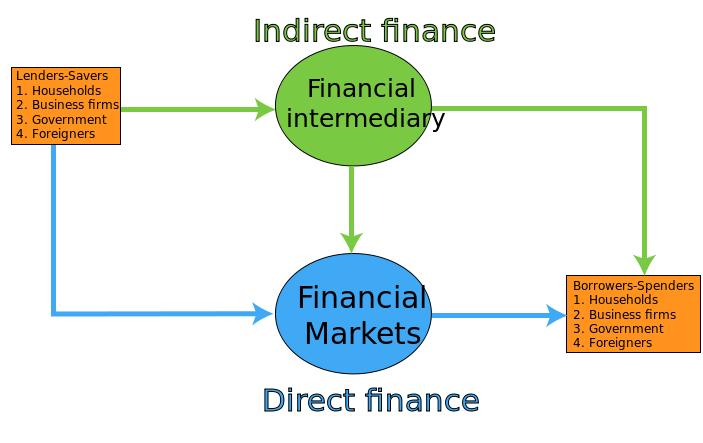
\includegraphics[width=0.8\textwidth]{FIs1.png}
	\end{figure}
\end{frame}
%==================================================================================
\begin{frame}
\frametitle{Financial intermediaries}
\framebox{Examples}
\hfill \break
\begin{itemize}
\item  Financial advisors
\item  Credit Union
\item Mutual funds/Investment trusts
\item  Insurance Companies
\item Pension funds
\item Commercial banks
\item Investment banks
\end{itemize}

\end{frame}

\begin{frame}
\frametitle{Financial intermediaries}
\begin{itemize}
\item Transform assets
\item Manage risks
\item Process information and monitor borrowers
\item Offer access to a payment system, public good
\end{itemize}


\framebox{Why care?} \hfill \break
\begin{itemize}
\item Facilitate economic growth: mobilising savings so that consumption can be higher in the future as a result of investments made today.
\item Global growth: Sending savings from countries with little room for further investment, to countries with more room than current savings can
satisfy.
\end{itemize}
\end{frame}


\begin{frame}
\frametitle{Why regulate?}

\textit{"We regulate finance over and above the way we regulate
other industries because finance exhibits market failures
that can have devastating consequences"}
\hfill \break
\begin{itemize}
\item financial market malfunction $\rightarrow$ the real economy $\Downarrow$
\item Example: Global financial crisis was triggered by problems in the US subprime mortgage market, but it led to German GDP shrinking by 6 percent in the first quarter of 2009 and the biggest drop in global trade since the 1930s.
\end{itemize}

\end{frame}
%-------------------------------------------------------------
\begin{frame}
\frametitle{Why regulate?}

Two principal drivers of market failures in finance that require
regulation
\textit{....there are others as well}
\hfill \break
\begin{itemize}
\item  Asymmetrical information
\begin{itemize}
\item Consumer protection - balance the interests of unsophisticated consumers of financial products and their sophisticated sellers
\end{itemize}
\item Social externalities
\begin{itemize}
\item  overall consequence of an activity is not captured
by the private interests of those involved in the activity.
\item $\rightarrow$ internalise with social taxes? (Pigouvian reponse)
\item .. costs of financial system failures are $>$ costs to the shareholders of a bank failure. $\Rightarrow$ regulatory
response: provide government insurance for depositors and higher capital requirements than banks would otherwise wish to hold
\end{itemize}
\end{itemize}
\end{frame}



%---------------------------------------------------------------------------
\begin{frame}
\frametitle{Banks are different}
\begin{itemize}
\item Banks accept \textit{deposits}
\item Banks lend to each other
\begin{itemize}
\item Bank A may borrow from Bank B to lend one of its customers a loan to
buy a car from a customer of Bank B.... \\
\framebox{why does this matter?}
\item when one shoe shop fails it might be good for another shoe shop (they do not lend to each other)
\item Failure of one bank $\rightarrow$ undermine other banks
\item Bank runs
\item A single bank failure could lead to a collapse of the financial system
\end{itemize}
\end{itemize}
\end{frame}


%__________________________________________________________________


\begin{frame}
\frametitle{Types of regulatory instruments}
\begin{itemize}
\item ceilings on deposit interest rates
\item restrictions on entry, size, and mergers
\item investment restrictions
\item deposit insurance
\item capital requirements
\item monitoring and bank supervision
\end{itemize}
\end{frame}

\begin{frame}
\frametitle{Tools for regulating the financial sector - grouped}
\begin{enumerate}
\item Prudential regulation.
\item Resolution tools
\item Oversight of clearing and settlement systems.
\item Conduct of business regulation
\end{enumerate}
\tiny{Source: https://www.imf.org/external/pubs/ft/wp/2009/wp0970.pdf}
\end{frame}


%--------------------------------------------------------------------------------


\section{The Architecture of Financial Regulation}\label{Sec::Chapter1}
%
%==================================================================================
%\begin{frame}
%	\begin{center}
%		\centering{\Large The Architecture of Financial Regulation\\ Chapter 1: Regulating Wall Street}
%	\end{center}
%\end{frame}

% --------------------------------------------------------------------------------

\begin{frame}

\textit{``Optimum regulation is the art of balancing the immeasurable against the unknowable''}
~\\
~\\
~\\
\pause
\frametitle{The Architecture of Financial Regulation}
There are four pillars of financial regulation:
\begin{itemize}\itemsep10pt
\item Encourage innovation and efficiency
\item Provide transparency
\item Ensure safety and soundness
\item Promote competitiveness in global markets
\end{itemize}
		\end{frame}

% --------------------------------------------------------------------------------

\begin{frame}
\frametitle{Limitations of Regulation}
Limitations to regulating the financial system:
\begin{itemize}\itemsep10pt
\item Asymmetric information\\
\quad \quad George Akerlof: Lemon's market
\item Costly state verification\\
\quad \quad Robert xTownsend: no disclosure until default, then full disclosure
\item Missing markets\\
\quad \quad Public goods: non-excludable/-diminishable/-rejectable
\end{itemize}
\end{frame}
%--------------------------------------------------------------
\begin{frame}
\begin{figure}
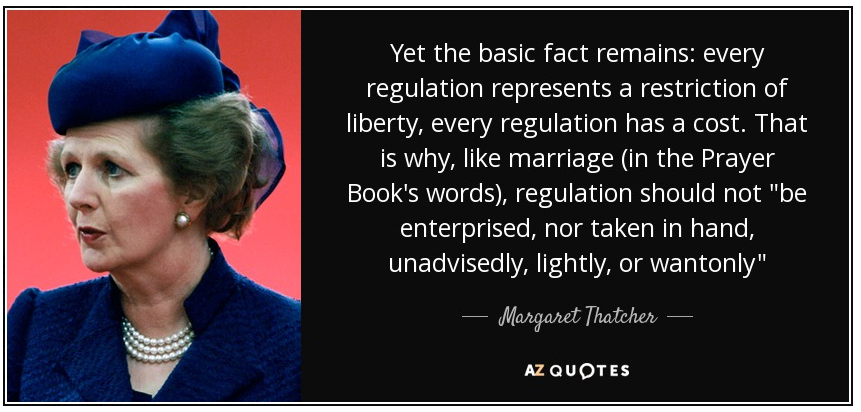
\includegraphics[width=\textwidth]{mthatch.png}
\end{figure}
\end{frame}

%-----------------------------------------------------------------
% ==================================================================
% ==================================================================
%

\begin{frame}
\begin{center}
 Day 1 Session 1.2\\
 Alternatives to Regulation
\end{center}
\end{frame}

\section{Alternatives to Regulation}
%
% ==================================================================
\begin{frame}
\frametitle{Alternatives to regulation}
Alternative approaches to financial regulation:
\begin{itemize}\itemsep10pt
\item Laissez-faire modification [Preferred by Wall-Street]
\item Glass-Steagall approach [Preferred by Interventionists]
\item Carve outs
\item Limit the size of financial conglomerates
\end{itemize}
\end{frame}

% ------------------------------------------------------------------

\begin{frame}
\begin{enumerate}
\item Modification of laissez-faire approach:
\begin{itemize}
\item Create appropriate tools for systemic risk regulation
\item Price implicit public subsidies
\item Create bankruptcy tools
\end{itemize}
\vspace{3mm}
\item Glass-Steagall approach:
\begin{itemize}
\item Legacy investment banks are converted into bank holding companies
\item Reverts them into broker-dealer status
\end{itemize}
\vspace{3mm}
\item Carve outs:
\begin{itemize}
\item Management of in-house hedge funds
\item Creation of off-balance-sheet affiliates
\item Large propriety trading positions in cash securities and derivatives
\item Principal investors in non-financial activities
\end{itemize}
\vspace{3mm}

\item Limit the size of financial conglomerates that incorporate commercial banking units
\end{enumerate}
\end{frame}

% ------------------------------------------------------------------

\begin{frame}{Legislation}
\frametitle{Legislation}
\begin{enumerate}
\item Dodd-Frank Wall-Street Reform and Consumer Protection Act:

\begin{itemize}
\item Created new agencies to help regulate the system
\item Takes into account the four pillars in financial regulation
\item Prohibits lending to non-banking corporations
\item Allows for emergency lending only to participants in an economic program
\item \mcdr{Fails to deal with shadow banking}
\end{itemize}
\vspace{3mm}

\item Consumer protection (BCFP):
\begin{itemize}
\item Bureau of Consumer Financial Protection is funded by the Federal Reserve
\item Regulates credit cards, mortgages and retirement and insurance investments
\end{itemize}
\end{enumerate}
\end{frame}


%==================================================================================




%======================================================================



%++++++++++++++++++++DAY1 Session 2



%+==========================================================
%

\begin{frame}
\begin{center}
 Day 1 Session 2 \\
 Financial intermediaries 1
\end{center}
\end{frame}

%-----------------------------------------------------------------
%======================================================================

\begin{frame}
	\begin{center}
		\centering{\Large Financial Intermediaries and Market Failures in Financial Markets}
	\end{center}
\end{frame}


%==================================================================================
%
\section{Recap: Financial Intermediaries}
%
%==================================================================================
\begin{frame}
	\frametitle{\insertsection}
	\begin{figure}[h]
		 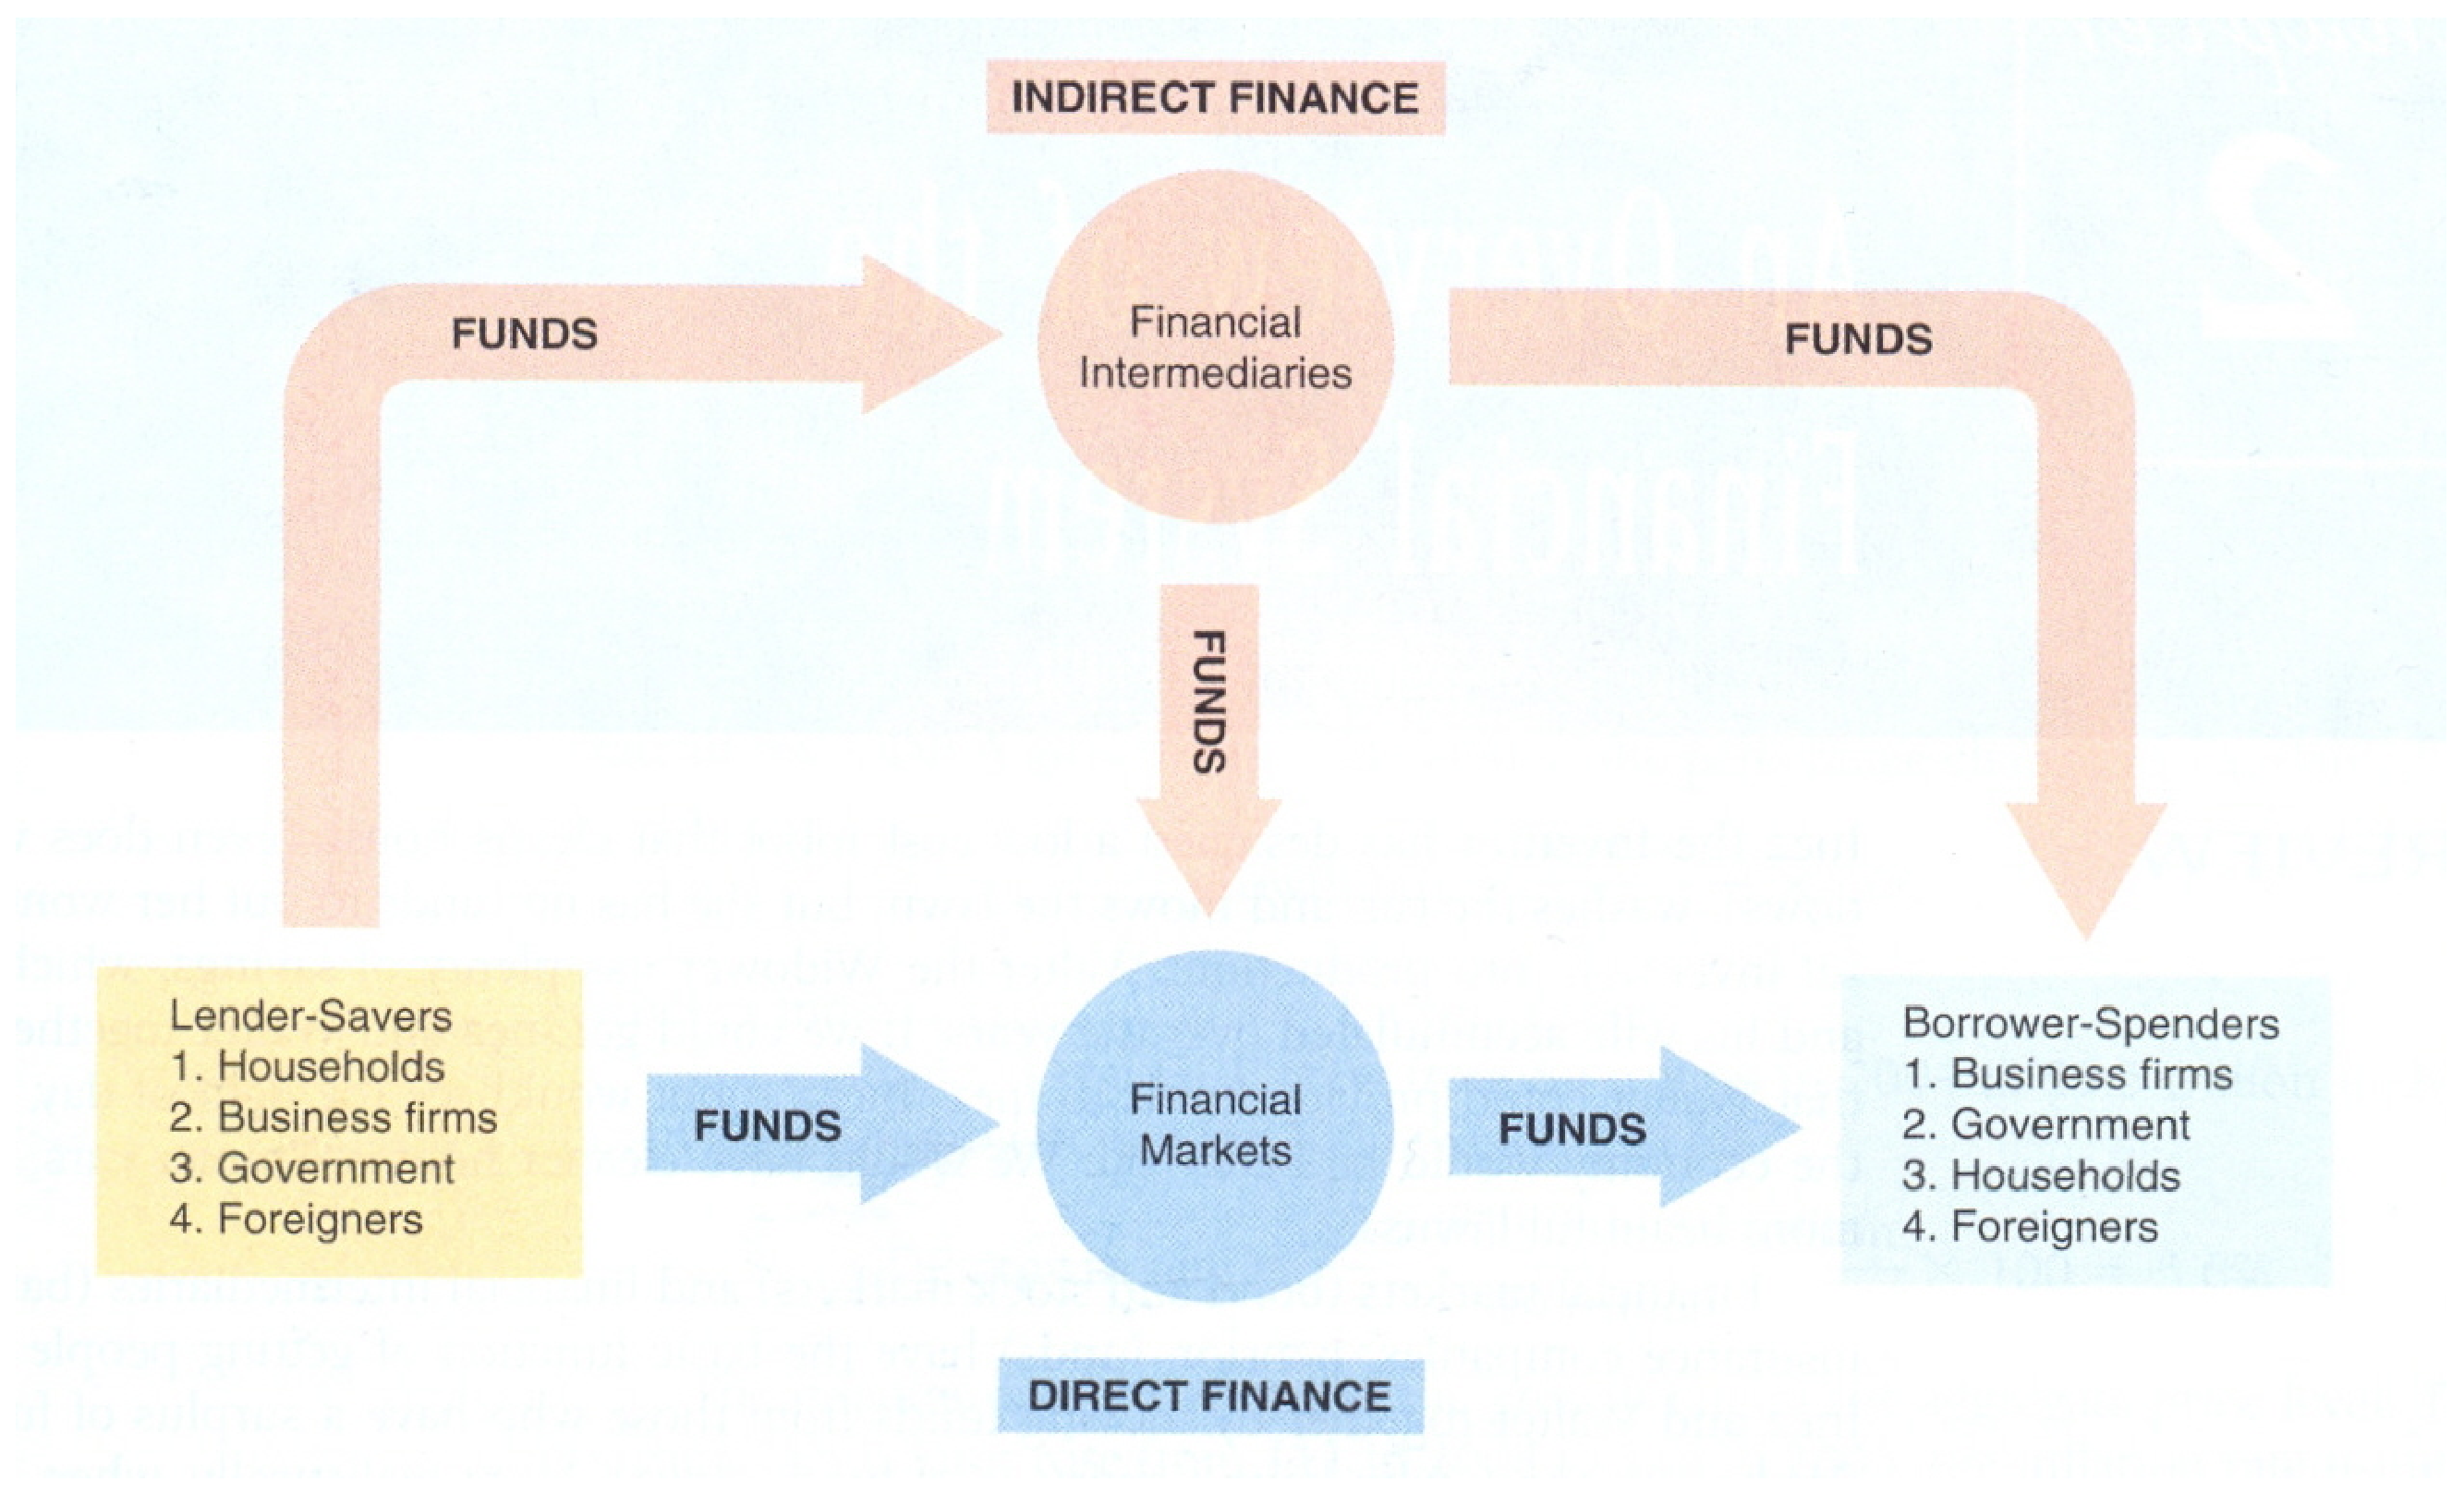
\includegraphics[width=0.8\textwidth]{Figures/intermediates.eps}
	\end{figure}
\end{frame}

% --------------------------------------------------------------------------------

\begin{frame}
\frametitle{\insertsection}
\textbf{a) Reducing Transaction Costs}
\begin{itemize}
\item FI have \textit{economies of scale}:
\par\smallskip
getting information about demanded and provided funds, assessing risks, bargaining, designing and enforcing contracts, buying/selling stock shares -- these tasks can be accomplished by FI with much lower transaction costs by specialized information processing abilities, large transaction volumes, specific human capital (expertise)
\item FI have \textit{economies of scope}:
\par\smallskip
FI provide additional services like risk diversification, optimizing portfolios, and consulting. Sometimes these services need the same infrastructure and the same human capital. Hence it \textit{may} reduce cost when one FI provides these services.
\end{itemize}
\end{frame}

% --------------------------------------------------------------------------------

\begin{frame}
\frametitle{\insertsection}
\textbf{b) Dealing with Risk:}
\begin{itemize}
\item Risks: Investment projects may fail, borrowers may become insolvent.
\item Reducing the risk by pooling them, reducing the risks arising from asymmetric information problems (see below).
\item Reducing the risk by selling assets with differert risk/return structures which are prefered by the
lender/saver (asset transformation, e.g. time deposit, fund shares).
\item Trading risky assets means that also risks are traded, all prices contain a ``risk premium''.
\end{itemize}
\end{frame}

% --------------------------------------------------------------------------------


\begin{frame}
\frametitle{\insertsection}
\textbf{c) Dealing with asymmetric information}
\begin{itemize}
\item \textbf{Adverse Selection:}
\begin{itemize}
\item Hidden characteristics of a potential borrower (e.g.) before a contracting.
\item Borrower knows his risk better than the lender.
\item If lender offers a contract which is optimal for a borrower with average risks, this may be unattractive for those with good risks. This may result in a market failure.
\end{itemize}

\item \textbf{Moral Hazard:}
\begin{itemize}
\item Hidden action of a borrower (e.g.) after contracting.
\item Borrower tales the money to engage in a prject that is undesireable for the lender. This reduces the probability for a successfully returned credit.
\end{itemize}

\item FI may alleviate this problem e.g. by screening, collaterals, optimal design of contracts. Again, they have the resources to do that with low transaction costs.
\end{itemize}
\end{frame}

% --------------------------------------------------------------------------------

\begin{frame}
\frametitle{\insertsection}

\textbf{Depository institutions (banks):}
\begin{itemize}
\item Accept deposits from individuals and institutions as liabilities, providing loans and mortgages as assets.
\item Example: Commercial banks, thrifts (saving and loans associations, mutual saving banks, credit unions).
\end{itemize}
% Deutsche Bank, Commerzbank, LBS

\textbf{Contractual savings institutions:}
\begin{itemize}
\item Accept premiums and contributions from government, firms and individuals as liabilities, investment in bonds, stocks and government securities.
\item Example: life insurance, pension funds, retirement funds
\end{itemize}
% Allianz, Debeka

\textbf{Investment intermediates:}
\begin{itemize}
\item Selling commerical stocks, bonds or shares as liabilities, providing business loans and investment in stocks and bonds as assets.
\item Example: Finance companies, mutual funds, private equity funds
\end{itemize}
% Morgan Stanley, Blackstone (in Germany it is part of investment banking)

\end{frame}

% --------------------------------------------------------------------------------

\begin{frame}
\frametitle{\insertsection}

\footnotesize
\hskip 0.5cm
\begin{tabular}{llll}
\hline
\textbf{Type of FI} & \textbf{Primary Liabilities} & \textbf{Primary Assets} & \textbf{Value}\\
\hline
\textit{Depository Institutions} & & & \\
\hline
Commercial Bank & Deposits & Loans, mortgages, & \\
                &          & bonds              & 6141 \\
Thrifts          & Deposits & Mortgages, & \\
                &          & consumer loans     & 2240\\
\hline
\multicolumn{2}{l}{\textit{Contractual saving Institutions}} & & \\
\hline
Life Insurance Companies & premiums & Bonds, mortgages & 3969\\
Fire/Caaualty Insur. Comp. & premiums & bonds, stocks & 1116\\
Pension funds & employer/employee & bonds, stocks & \\
              & contributions & & 4330\\
Gov. retirement funds & employer/employee & bonds, stocks & \\
              & contributions & & 2046\\
\hline
\textit{Investment Intermediates} & & & \\
\hline
Finance Companies & commercial papers, & loans & \\
                  & stocks, bonds & & 1385 \\
Mutual Funds & issued shares & bonds, stocks & 4969\\
Money market mutual funds & issued shares & money market instr. & 1912\\
\hline
\end{tabular}
\par
{\tiny (US Data 2004 , Bill. Dollar, source: Mishkin (2006), Tables 1 and 2)}
\end{frame}
%+==========================================================
%
%======================================================================



%++++++++++++++++++++DAY1 Session 3



%+==========================================================
\begin{frame}
\begin{center}
 Day 1 Session 3 \\
 A Bank's balance sheet
\end{center}
\end{frame}


%
\section{Banks as Financial Intermediaries}
%

% ------------------------------------------------------------------
\begin{frame}
\frametitle{What is a balance sheet}
\begin{itemize}
\item A summary of the assets and liabilities of a business (bank)
\item A snapshot of assets and liabilities at a particular point in time
\item A balance sheet always balances - double entry bookkeeping
\begin{itemize}
\item Assets are \textit{owned} by the bank
\item Liabilities are \textit{owed} by the bank
\end{itemize}
\end{itemize}


\end{frame}





%-----------------------------------------------------------------

% ==================================================================
\begin{frame}
\frametitle{\insertsection}

\begin{center}
\textit{The Bank's Balance Sheet}
\end{center}
\par\medskip

\begin{tabular}{l|l}
\hline
Assets & Liabilities\\
\hline
\begin{minipage}{5cm}
\begin{itemize}
\item Reserves {\small (required, excess)}
\item Cash
\item Securities/Bonds
\begin{itemize}
\item firm bonds
\item governmental bonds
\end{itemize}
\item Loans
\begin{itemize}
\item industrial
\item consumer
\item real estate
\item inter-bank
\item other
\end{itemize}
\item Other assets\\
{\small (e.g. physical assets)}
\end{itemize}
\end{minipage}
&
\begin{minipage}{5cm}
\begin{itemize}
\item (Checkable) Overnight deposits
\item Nontransaction desposits
\begin{itemize}
\item Time deposits
\item Redeemable deposits\\(saving accounts)
\end{itemize}
\item Borrowings
\begin{itemize}
\item Inter-bank loans
\item Central bank loans
\item Other
\end{itemize}
\item Bank Capital
\end{itemize}
\end{minipage}\\
\hline
\end{tabular}
\end{frame}


%---------------------------------------------------------------
\begin{frame}
\frametitle{Stylised balance sheet - commercial bank}
\begin{figure}
	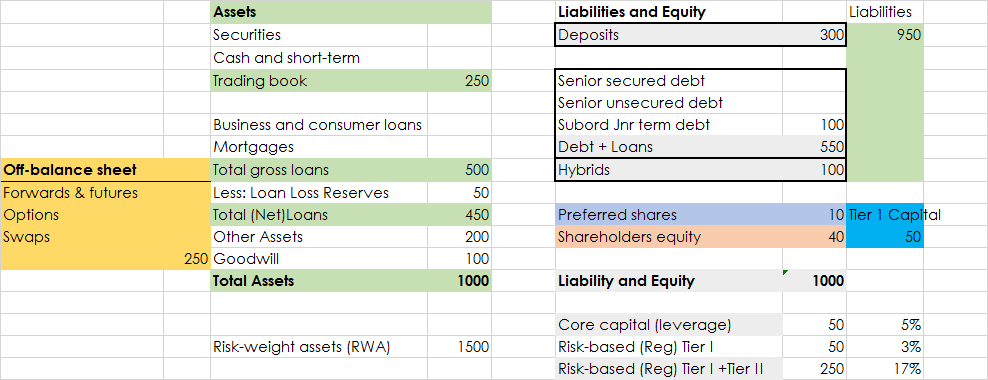
\includegraphics[width=1\textwidth]{TotalBS.png}
\end{figure}

\end{frame}


%-----------------------------------------------------------------
%-------------------------------------------------

\begin{frame}
\frametitle{Commercial banks vs investment banks}
\begin{figure}
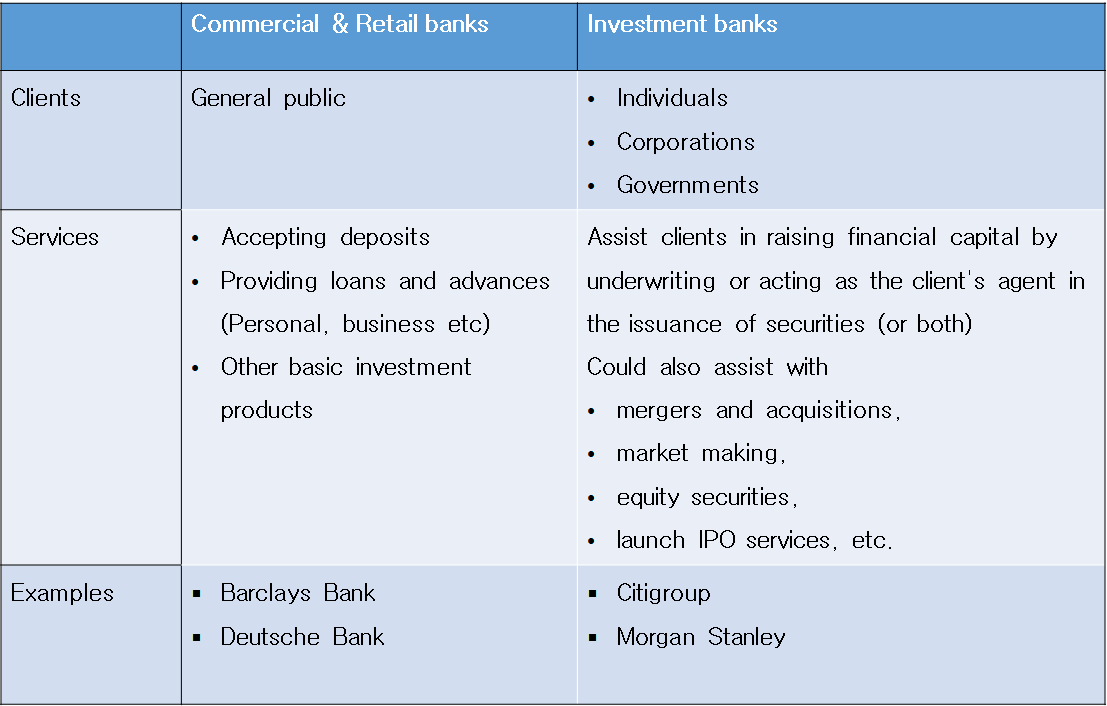
\includegraphics[width=\textwidth]{commret.png}
\end{figure}


\end{frame}


%==============================i====================================================

%======================================================================



%++++++++++++++++++++DAY1 Session 4 and 5



%+==========================================================
%

\begin{frame}
\begin{center}
 Day 1 Sessions 4 and 5
 Banks as financial intermediaries - Liquidity management, asset management and liability management and  adverse selection
\end{center}
\end{frame}

% =================================================================
%
\section{Banks as financial intermediaries}
%
% =================================================================


%-----------------------------------------------------------------
% ==================================================================
\begin{frame}
\frametitle{\insertsection}

\textbf{a) Liquidity Management}

\begin{itemize}
\item For deposit outflows the bank needs liquid assets like cash or reserves.

\item If there are not enough liquid positions on the asset side the bank needs expensive overnight loans or has to sell other assets, or it becomes illiquid. These are costs of deposit outflows.

\item Problem: If customers receive a signal of liquidity problems they also wish to draw their deposits. This enforces the liquidity problem and may lead to bankruptcy.

\item Liquidity management has to balance the liquidity of assets with the deposit position on the liability side. More generally: Given a probability distribution of inflows and outflows on the liability side, the asset side should be structured to meet the obligations to the depositors.
\end{itemize}
\end{frame}

% ------------------------------------------------------------------

\begin{frame}
\frametitle{\insertsection}

\begin{itemize}
\item The higher the expected deposit outflows  and/or the higher the cost of deposit outflows are the more excess reserves are required.
\end{itemize}
\par\medskip

\textbf{b) Asset Management }

\begin{itemize}
\item Management of risk and return of the assets (portfolio approach). Finding the mix of risky and riskless assets with the highest expected utility (assumption: risk aversion).

\item The liquidity considerations (see a)) can be seen as an additional restriction to portfolio management.

\item Portfolio theory is a core concept in (financial) economics. Details are given in the next subsection.
\end{itemize}
\end{frame}

% ------------------------------------------------------------------

\begin{frame}
\frametitle{\insertsection}

\textbf{c) Liability management}

\begin{itemize}
\item Deposits are not ``given'' and not the only source of funds. Decision how to acquire which types of liabilities.

\item Differences of liabilities:
\begin{itemize}
\item Hows fast could an additional liability be acquired?
\item Probability of outflows
\item Costs = interest rates (e.g. for time deposits, for inter-bank or central bank loans)
\end{itemize}

\item Development of new financial instruments (e.g. certificates of deposits (CD) which are similar to bonds)
\end{itemize}

\end{frame}

% ------------------------------------------------------------------

\begin{frame}
\frametitle{\insertsection}

\textbf{d) Bank Capital Management}

\begin{itemize}
\item Most assets have risks: Credits may fail, bonds prices may fall. Hence, the value of the asset side is volatile.

\item With a certain probability the losses of the asset side may exceed the bank capital: the bank becomes insolvent.

\item Actual development: Large bank crisis in the USA in 2008. About 500 Billion Dollar asset values (especially housing loans and mortgages) had to be written off.

\item The higher the bank capital (in percent of the liability side), the lower is the risk of insolvency.

\item But: The return on equity (RoE) of the bank owners (return on assets / bank capital) is c.p. lower when the bank capital has a higher share of the liability side $\rightarrow$ trade-off!
\end{itemize}

\end{frame}


% =================================================================
%
\section{Adverse Selection Problems}
%
% =================================================================
\begin{frame}
\frametitle{\insertsection}

\textbf{Information Asymmetries:}
\small
\begin{itemize}
\item before contracting: hidden characteristics $\rightarrow$ adverse selection
\par\medskip
\begin{itemize}
\item buying shares or bonds of a firm $\Rightarrow$ characteristics are not known to the buyer
\item providing a loan to a borrower with unknown ability to pay back the loan (credit risk)
\par\medskip

\item [$\Rightarrow$] decision is based on expectations about the characteristics
\item [$\Rightarrow$] expectations are built on prior and posterior information
\item [$\Rightarrow$] limited possibilities to reveal the unknown characteristics
\item [$\Rightarrow$] Pooling vs. Separating equilibria
\end{itemize}

\item after contracting: hidden action $\rightarrow$ moral hazard
\par\medskip

Firm uses the funds for financing projects which are more risky than indicated in the negotiation with the  lender or buyer of a share. The latter can not observe this, but they can expect that there is an incentive for moral hazrd.
\end{itemize}
\end{frame}

% ------------------------------------------------------------------

\begin{frame}
\frametitle{\insertsection}

\textbf{Markets for Lemons}

\begin{itemize}
\item Akerlof, G.A. (1970), The Market for Lemons: Qualitative Uncertainty and the Market Mechanism. \textit{Quarterly Journal of Economics} Vol. 84, 499-500.
\item Wolfstetter, E.  (1999), \textit{Topics in Microeconomics}. (Chapter 9.2.1)
\end{itemize}

Nobel Prize 2001 to George A. Akerlof, A. Michael Spence, Joseph E. Stiglitz "`for their analyses of markets with asymmetric information"'.
\par\medskip

Foundation of market imperfections or market failures due to information asymmetries.

\end{frame}

% ------------------------------------------------------------------

\begin{frame}
\frametitle{\insertsection}

The original version: Market for used cars
\begin{figure}

\includegraphics[width=0.6 \textwidth]{Cars.png}
\end{figure}
\end{frame}


\begin{frame}
\frametitle{Market for used cars}
\begin{itemize}
\item Cars have a different quality $q$ (from ``very good'' $q=b$ to ``bad'' $q=0$, bad cars = ``lemons'')
\item The seller is privately informed about the quality $q\in[0,b]$.
\item The seller will accept any price $p\geq q$.
\item The buyer is willing to pay any price $p\leq \alpha\cdot q$ with $\alpha>1$.
\item For any given $q$ there exists a price $\in[q,\alpha q]$ where buyer and seller mutually benefit from the deal.
\par\medskip

\item \textbf{But:} The buyer is not able to observe $q$\\ $\Rightarrow$ building expectations $E[q]$.
\end{itemize}

\end{frame}

% ------------------------------------------------------------------

\begin{frame}
\frametitle{\insertsection}

Assume that the quality $q$ is \textit{uniformly distributed} on $[0,b]$. This is known by the buyer.
For any used car the expected quality is hence $E[q]=b/2$. Therefore
$$
p(E[q])\leq \alpha\cdot\frac{b}{2}
$$

Two cases:
\begin{itemize}
\item \textit{Case 1:} $\alpha \geq 2$. Then the buyer is willing to pay $p\geq b$ and all cars will be sold.
\item \textit{Case 2:} $1<\alpha<2$. Then the market breaks down!
\end{itemize}

\end{frame}

% ------------------------------------------------------------------

\begin{frame}
\frametitle{\insertsection}

Market breakdown:
{\small
\begin{itemize}
\item For $\alpha<2$ the buyer will never pay $p=b$.
\item No high quality cars ($q=b$) will be sold. They can be removed from the interval (e.g. $q\in[0,b-\epsilon]$).
\item This can be anticipated by the buyer. The expected average quality decreases (e.g. $E[q]=(b-\epsilon)/2$).
\item The willingness to pay also decreases.
\item The remaining best quality cars leave the market.
\item and so forth... (``race to the bottom'')
\end{itemize} }
\end{frame}

% ------------------------------------------------------------------

\begin{frame}
\frametitle{\insertsection}

Or in another way:

\begin{itemize}
\item Assume an arbitrary market price  $p>0$. Obviously there are only sellers i the market with $q_i\in[0,p]$.
The average quaility is hence $E[q]=\frac{p}{2}$.

\item This is known by the buyers. The are willing to pay maximum $p(E[q])=\alpha/2\cdot p$.

\item For $\alpha<2$ this is lower than the market price and no deal comes about.
\end{itemize}

\end{frame}

% ------------------------------------------------------------------

\begin{frame}
\frametitle{\insertsection}

\textbf{Financial Markets:}

\begin{itemize}
\item Firm needs funds to finance a risky project. The funds can be obtained by debt or equity. Assume that the firm demands for a loan $L$.

\item The (risk neutral) firm is willing to pay an interest rate $i_L$ which does not exceed the expected return of the project $r$.

\item The bank will provide the loan $L$ when the interest rate covers at least the interest rate for a secure asset $i_S$ plus the risk premium $RP$.

\item Assume that the loan is either returned successfully with probability $1-p$ or it fails completely with probability $p$. The minimum risk premium is therefore:
\begin{align}
L(1+i_S) &= L(1+i_L)(1-p)+0\cdot p\\
\Rightarrow\quad
RP=i_L-i_S &= \frac{p}{1-p}(1+i_S)
\end{align}

\end{itemize}

\end{frame}

% ------------------------------------------------------------------

\begin{frame}
\frametitle{\insertsection}

\begin{itemize}
\item Problem: $p$ is \textit{private information} of the firm = not known by the bank!

\item Offering a loan contract with an interest rate $i_L$ (and risk premium) based on the \textit{expected} probability $E[p]$ taken from a prior distribution of risks.

\item Typically the expected return and the risk of investment projects are positively correlated.
Firms with \textit{profitable low risk projects} with
$$
r<i_S+\frac{E[p]}{(1-E[p])}(1+i_S)
$$
will not get a loan contract!

\item The remaining projects are hence more risky which leads to an increase of $E[p]$ $\Rightarrow$ a similar mechanism as in the ``market for lemons'' example applies.
\end{itemize}

\end{frame}

% ------------------------------------------------------------------

\begin{frame}
\frametitle{\insertsection}

\textbf{Credit Rationing:}
\par\medskip

Adverse Selection Effect: With an increasing interest rate more and more good (= low risk) projects leave the market and the expected risk increases:
$$
E[p]=E[p(i_L)],\qquad \frac{dE[p(i_L)]}{di_L}>0
$$
Profit maximizing bank:
\begin{align}
\max_{i_L} \pi &= (1-E[p(i_L)])(1+i_L)L\\
\Rightarrow\quad
\frac{d\pi}{di_L} &= -\frac{dE[p(i_L)]}{di_L}(1+i_L)L+(1-E[p(i_L)])L=0\\
\Rightarrow\quad
i_L^* &= \frac{(1-E[p(i_L)])-\frac{dE[p(i_L)]}{di_L}}{\frac{dE[p(i_L)]}{di_L}}
\end{align}
\end{frame}

% ------------------------------------------------------------------

\begin{frame}
\frametitle{\insertsection}

What are the consequences?

\begin{itemize}
\item The profits do not monotonously increase with market interest rate $i_L$.

\item If loans demand increases \textit{there is not neccessarily a Walrasian adjustment of the equilibrium interest rate! }

\item The demand side of the loans market will be rationed.

\item Existence of \textit{rationing equilibria}.

\item The notional plans of the firms cannot be fulfilled \\
$\Rightarrow$ spillover to other markets
\begin{itemize}
\item  e.g. markets for bonds or equities to finance the project
\item  e.g. markets for investment goods
\end{itemize}

\end{itemize}

\end{frame}

% ------------------------------------------------------------------

\begin{frame}
\frametitle{\insertsection}

Literature:
\par\bigskip

\begin{itemize}
\item Stiglitz, J., Weiss, A. (1981), Credit Rationing in Markets with Imperfect Information. \textit{American Economic Review} 71, 393-410.
\item Greenwald, B., Stiglitz, J., Weiss, A.  (1984), Information Imperfections in the Capital Market and Macroeconomic Fluctuations. \textit{American Economic Review} 74, 194-199.
\end{itemize}
\par\bigskip

Note:

\begin{itemize}
\item The problem of rationing may be (partially) overcome e.g. by collaterals.

\item The problem may also occur in bonds and stock markets: The price which the inital buyer is willing to pay reflects his uncertainty about the risk type of the firm!
\end{itemize}

\end{frame}

% ------------------------------------------------------------------

\begin{frame}
\frametitle{\insertsection}

There are different ways how to solve or to alleviate the problem:

\begin{itemize}
\item Providing  better information = decreasing information asymmetry
\begin{itemize}
\item \textit{Screening:} The less informed agent has an incentive
\begin{itemize}
\item     to collect information by himself
\item     to buy additional information supplied by other agents
\item     to provide different contracts with self-selection effects
\end{itemize}
\item \textit{Signalling:} The privately informed agent has an incentive to provide a trustworthy (costly) signal about his characteristics.
\item \textit{Governmental Regulation}
\end{itemize}

\item Collateral and Net Worth
\par\smallskip
  The information asymmetry is not resolved but has minor consequences since in case of a failed project the return of the loan do not fail.
\end{itemize}

\end{frame}

% ------------------------------------------------------------------

\begin{frame}
\frametitle{\insertsection}

\textbf{Screening by collecting information}

\begin{itemize}
\item High information costs, especially for lenders with low expertise.

\item Bank as a financial intermediate with expertise and specialized human capital reduces such information costs:
\begin{itemize}
\item Multiple lender of funds $\Rightarrow$ bank deposits
\item Bank is pooling the risks and guarantees the depositor an interest rate
\item Screening costs of multiple non-specialized lenders are reduced and transferred to the bank
\item The bank as the intermediate lender faces a lower information asymmetry
\end{itemize}

\item The existence of a professional banking system is a prerequisite for a working credit market (crucial for developing countries).
\end{itemize}
\end{frame}

% ------------------------------------------------------------------

\begin{frame}
\frametitle{\insertsection}

\textbf{Screening by buying information provided by others}

\begin{itemize}
\item Rating agencies (e.g. Standard \& Poors, Moody): (Large) Borrowers are rated according to a standardized scale (see Mishkin (2006), chapter 6, p.123)

% \item In Germany: SCHUFA (Schutzgemeinschaft für allgemeine Kreditsicherung)
\end{itemize}

\textbf{Problems:}

\begin{itemize}
\item \textit{Free-rider problem} since information is a non-rival good. Once, when information is made public, there is no incentive anymore to pay for it.

\item How \textit{trustworthy} is that information?  Moral Hazard problem of information providing institutions since the customer (e.g. bank) is not able to asses the reliability of the information.
\end{itemize}
\end{frame}

% ------------------------------------------------------------------

\begin{frame}
\frametitle{\insertsection}

\textbf{Governmental Regulation:}
\par\medskip

If investors need financial funds, e.g. by demanding credits or selling bonds or stocks, they can be forced by law to provide some information to reduce the information asymmetry. E.g.
\begin{itemize}
\item adhere standard accounting principles
\item providing information about the balance sheet and other (financial) indicators like sales, earnings, assets
\item in case of stock markets: publish relevant informations regularly, annual meeting of shareholders etc.
\end{itemize}
\label{govreg}
\end{frame}

% ------------------------------------------------------------------

\begin{frame}
\frametitle{\insertsection}

\textbf{Signalling:}

\begin{itemize}
\item A firm with a low risk project has an incentive to provide a signal so that the lender is informed about the low risk (and charging a low risk premium).

\item If signalling should make sense...
\begin{itemize}
\item[(a)] the signal must  be costly
\item[(b)] there must exist signals that are too expensive for a high risk firm but not too expensive for low risk firms $\Rightarrow$ discrimination is possible.
\end{itemize}

\item Otherwise high risk firms have an incentive to \textit{imitate} the signal so that signalling provides no information (pooling equilibrium).
\end{itemize}
\end{frame}

% ------------------------------------------------------------------

\begin{frame}
\frametitle{\insertsection}

Signalling means ``building reputation''. Reputation signals (e.g.):

\begin{itemize}
\item Loans have been successfully returned in the past.
\item Projects are financed also with equity capital.
\item Firm provides voluntarily more sensitive information than required by law.
\item Firm has valuable assets ($\rightarrow$ similar to collaterals).
\end{itemize}
\par\bigskip

This may be a problem for new and small firms.
\end{frame}

% ------------------------------------------------------------------

\begin{frame}
\frametitle{\insertsection}

\textbf{Collaterals:}

\begin{itemize}
\item In case of failure of the investment project the investor has other assets which can be sold to meet the debt obligations.

\item The borrower must prove that he has such collaterals before signing the credit contract.

\item The credit contract may include the obligation that a certain asset must not sold before the credit is returned successfully.

\item The credit contract includes that lender automatically becomes the owner of an asset in case of a credit failure.

\item The credit contract includes that the lender has property rights on the asset which are returned to the borrower in case of a successfully returned credit $\Rightarrow$ mortgages (e.g. in case of housing, real estate)
\end{itemize}
\end{frame}

% ------------------------------------------------------------------

\begin{frame}
\frametitle{\insertsection}

Collaterals $C$ lower the risk premium:
\begin{align}
L(1+i_S) &=L(1+i_L)(1-p)+pC\\
\Rightarrow\quad
RP=i_L-i_S &=\frac{p}{1-p}(1+i_S)-\frac{p}{1-p}\frac{C}{L}
\end{align}
with $C=\arg\max\{0,(1+i_S)L\}$. In case of $C=L(1+i_S)$ there is no credit risk for the lender anymore.
\par\medskip

\textbf{Problems:}
\begin{itemize}
\item Providing collaterals is costly (e.g. opportunity costs).
\item The access to collaterals is limited (e.g. start-up companies).
\item The value of collaterals may be uncertain (see the recent housing crisis in the U.S. -- dramatic decrease of house prices = decrease of the value of collaterals)
\end{itemize}
\end{frame}

% ------------------------------------------------------------------

\begin{frame}
\frametitle{\insertsection}

Literature on Collaterals:
\par\bigskip

\begin{itemize}
\item Bester, H. (1985), Rationing in Credit Market with Imperfect Information. \textit{American Economic Review} 75, 850-855.

\item Besanko, D., Thakor, A. V. (1987), Collateral and Rationing: Sorting Equilibria
in Monopolistic and Competitive Credit Markets. \textit{International Economic Review} 28, 671-689.
\end{itemize}
\end{frame}

% ------------------------------------------------------------------


%======================================================================
%======================================================================
%
%-------------------------------------------------------------------------
%Day one perhaphs last session

%======================================================================
%-----------------------------------------------------------------------
\begin{frame}
\begin{center}
 Day 1 Session 6\\
History of US banks and establishing the US Fed
\end{center}


\end{frame}

%======================================================================

\begin{frame}
\frametitle{US banks}
\begin{itemize}
\item No American banks as late as 1781
\item Alexander Hamilton writes to Congress’s superintendent of finance, Robert Morris, that \textit { “Most commercial nations have found it necessary to institute banks and they have proved to be the happiest engines that ever were invented for advancing trade.” }. Hamilton recommended that a bank be founded.
\item Morris persuaded Congress to charter the new nation’s first bank, \textit{the Bank of North America} located in Philadelphia in 1782.
\item Three years later, Boston merchants founded the Massachusetts Bank and Hamilton became a founder of the Bank of New York.
\item The irony: establishment of the \textit{First Bank of the United States} in 1791

\end{itemize}

\end{frame}

%---------------------------------------------------------------
\begin{frame}
\frametitle{US banks ... continued}
\begin{itemize}
\item First Bank of the United States was opposed for being unconstitutional
\item many fearing that it relegated undue powers to the federal government $\Rightarrow$ its charter was not renewed in 1811
\item War of 1812 $\Rightarrow$ government turning to state banks for finance... followed by over-expansion of credit
\item financial order needed to be reinstated
\item obtaining an official legislative charter was highly political



\end{itemize}
\end{frame}

\begin{frame}
\frametitle {Era of free banking}
\begin{itemize}
\item A new era of “free banking” emerged with a number of states passing laws in 1837 that abolished the requirement to obtain an officially legislated charter to operate a bank, and by 1860, a majority of states had issued such laws.
\item Anyone could operate a bank, one of the conditions was that all notes issued were back by proper security
\item still it did not guarantee immediate redemption in specie (gold or silver)
\item era of free banking suffered from financial instability with several banking crises occurring
\item  a disorderly currency characterized by thousands of different bank notes circulating at varying discount rates


\end{itemize}
$\Rightarrow$ The free banking era - characterized as it was by a complete lack of federal control and regulation - came to an end with the National Banking Act of 1863

\end{frame}

\begin{frame}
\begin{itemize}
\item National Banking Act of 1863 aimed to replace the old state banks with nationally chartered ones.
\item Office of the Comptroller of the Currency (OCC) was created to issue these new bank charters as well oversee that national banks maintained the requirement to back all note issuance with holdings of US government securities
\item new national banking system helped return the country to a more uniform and secure currency
\item growing complexity of the U.S. economy highlighted the inadequacy of an inelastic currency
\item frequent financial panics occurring throughout the rest of the nineteenth century
\item occurrence of the bank panic of 1907, it had become apparent that America’s banking system was out of date





\end{itemize}
\end{frame}


%----------------------------------------------------------------
\begin{frame}
\frametitle{Establishing the US Fed}

\begin{itemize}
\item  Congress created a new central bank, the Federal Reserve System (Fed) in 1913, after three-quarters of a century without a central bank - a period punctuated by a number of banking crises.
\item by end 1914 the twelve regional Reserve Banks, coordinated by the Federal Reserve Board in Washington, DC, were open for business.
\end{itemize}
\begin{figure}
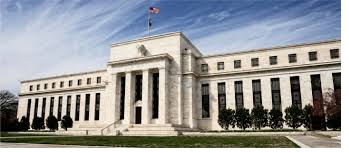
\includegraphics[]{Fed.png}
\end{figure}
\end{frame}


% \begin{frame}
% \begin{center}
% Paper to be discussed: %http://www.jstor.org/stable/1911459?seq=1#page_scan_tab_contents
% JOURNAL ARTICLE
% Pareto Optima and Competitive Equilibria with Adverse Selection and Moral Hazard
% Edward C. Prescott and Robert M. Townsend
% Econometrica
% Vol. 52, No. 1 (Jan., 1984), pp. 21-46
% \end{center}
% \end{frame}

%======================================================================








%++++++++++++++++++++DAY2 Session 1



%+==========================================================
\begin{frame}
\begin{center}
 Day 2 Session 1 \\
 History of US legislation
\end{center}
\end{frame}

%---------------------------------------------------------------------

\begin{frame}
\frametitle{History of US legislation}




FIs today specialize in a certain type of activity, but this has not always been the case.
It was not until after the crash of 1929 that these two types of banking began to operate separately.

\end{frame}

%--------------------------------------------------------------------

\begin{frame}
\frametitle{Background to US regulatory changes -\\ Leading up to 1929}
\begin{itemize}
\item Roaring Twenties
	\begin{itemize}
	\item Unprecedented economic boom in the US
    \item Mass production in manufacturing, telecommunication, movie and chemical sectors
    \item Population moved into cities to acquire jobs in these industries
    \item Americans - cash flush - invest in the stock market and deposit into banks
    \item Banks were opening at a rate of 4-5 per day (!)
	\end{itemize}

\end{itemize}

\end{frame}
%-----------------------------------------------------------------
\begin{frame}
\begin{figure}
	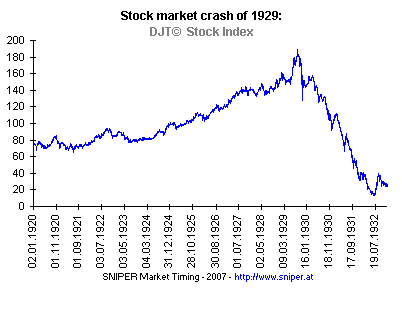
\includegraphics[width=1\textwidth]{Stockmarket.png}
\end{figure}

\end{frame}
%-------------------------------------------------------------------

\begin{frame}
\frametitle{Background to US regulatory changes - \\ The Great Depression (1929 - 1941)}
\begin{itemize}
\item 1929 stock market crash
	\begin{itemize}
	\item Stock market peaked on 3 Sept 1929
	\item 29 October 1929 - 40 per cent down. $\rightarrow$ Black Tuesday. Investors lost 14 billion dollars in a single day.
	\end{itemize}
\item Banks
\begin{itemize}
\item Banks lent money to investors to buy stock
\item Margin requirements were low
\item Banks were allowed to speculate and buy stocks for themselves
\item $\rightarrow$ The crash put a lot of pressure on banks
\end{itemize}
\end{itemize}


\end{frame}
%----------------------------------------------------------------------


\begin{frame}
\frametitle{Background to US regulatory changes - \\ The Great Depression (1929 - 1941)}
Once the selling began, more selling was needed to satisfy margin calls and liquidity requirements for banks....
\\

\begin{itemize}
\item Bank runs
\begin{itemize}
\item No guarantees on cash at the bank
\item People feared that their bank would collapse
\item Some banks were not able to fulfill the requests for withdrawal and closed their doors to people
\item $\downarrow$ lending to businesses and consumers
\item $\rightarrow$ more people need to withdraw money
\item paper money was backed by gold
\item people kept money under their mattresses
\end{itemize}

\end{itemize}

\end{frame}
%------------------------------------------------------------------
\begin{frame}
\begin{figure}
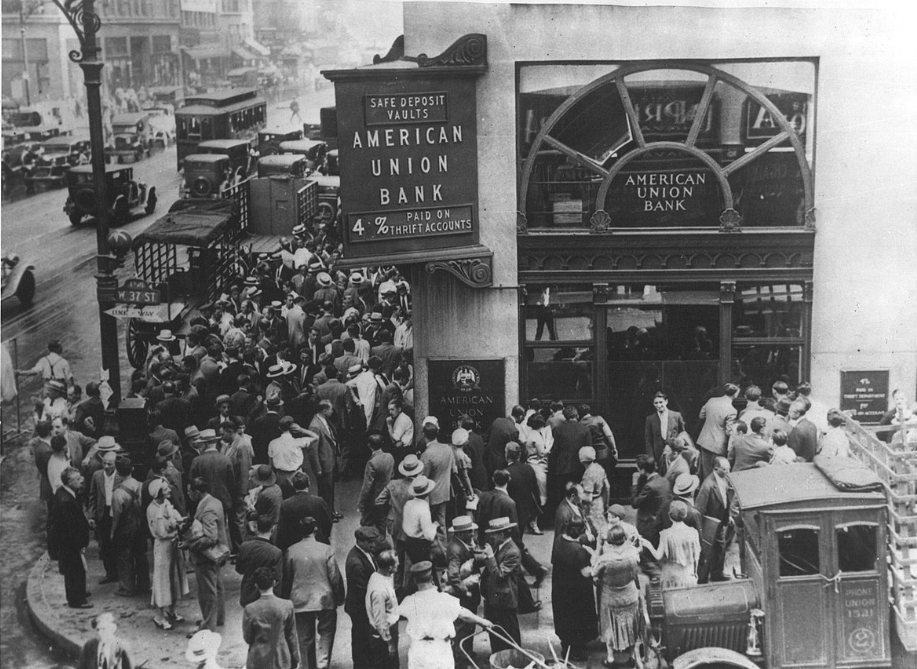
\includegraphics[width=1\textwidth]{Bankrun.png}
\end{figure}
\end{frame}



%-------------------------------------------------------------------
\begin{frame}
\frametitle{The US Federal Reserve and the Great Depression}

\begin{itemize}
\item The government began to increase interest rates, in 1929, from 3.5$\%$ to 5$\%$.
\item Money supply not stabilised - supply fell by 30$\%$ between 1929 and 1933
\item prices dropped
\item banks failed
\item $\Rightarrow$ deflation
\item $\Rightarrow$ No confidence in banking sector
\item Focus was on maintaining the gold standard - sufficient gold reserves to meet the demands of the depositor, and adequate demand for currency

\end{itemize}


\end{frame}

%---------------------------------------------------
\begin{frame}
\frametitle{Great Depression Effects on the Economy}
\begin{itemize}
\item \textbf{Higher unemployment} By 1933, the unemployment rate had climbed from 3$\%$ to 25$\%$
\item \textbf{Lower income} On average incomes were reduced by 40 $\%$
\item \textbf{Deflation}
\item \textbf{Increased foreclosures} By 1934, nearly one-half of all residential loans were delinquent and over 1 million families lost their farms
\item \textbf{Banks close} In 1933 alone, more than 4 000 banks closed
\item \textbf{Hollywood} actually did very well during this period of time - the Hollywood film industry. It is thought that people went to the movies because, for a brief time while at the movie, they could forget their many hardships :)

\end{itemize}
\end{frame}

%-------------------------------------------------------------------
\begin{frame}
\frametitle{Bank Holiday of 1933}
An effort to stem bank failures and ultimately restore confidence in the financial system
\begin{itemize}
\item 36 hours after taking office in March 1933, President Roosevelt ordered the suspension of all banking transactions, effective immediately
\item For an entire week, Americans would have no access to banks or banking services.
\item Before banks could reopen, there needed to be agreement on whether or not to “weaken the link between gold and note issue” (Meltzer 2003, 423)
\item The crisis began to subside on 9 March, when Congress passed the Emergency Banking Act.
\item On March 13, member banks in Federal Reserve cities received permission to reopen.
\item By March 15, banks controlling 90$\%$ percent of the country’s banking resources had resumed operations and deposits far exceeded withdrawals.... the worst of the banking crisis seemed to be over.
\end{itemize}
\end{frame}




%---------------------------------------------------------------------

\begin{frame}
\frametitle{Policy changes during the great depression}

Role of the US Government changed dramatically

\begin{itemize}
\item Banking Act of 1933
\begin{itemize}
\item Glass-Stegall Act - breaks connection between commercial and investment banks
\item Federal Deposit Insurance Corporation (FDIC) - insure bank deposits
\item Regulation Q - outlawed the payment of interest on checking accounts and also placed ceilings on the amount of interest that could be paid on other deposits
\end{itemize}

\item 1933: The US goes off the gold standard
\item 1934: Securities and Exchange Act - helped to police activities related to the selling of securities
\item 1935: Social Security Act - assistance to the unemployed, handicapped and elderly
\item  Banking Act of 1935 - fully insured balances up to $\$$5,000 and provided no insurance for balances above that amount
\end{itemize}




\end{frame}

\begin{frame}
\begin{figure}
\frametitle{President Franklin D. Roosevelt signs the Glass-Steagall banking bill in 1933}
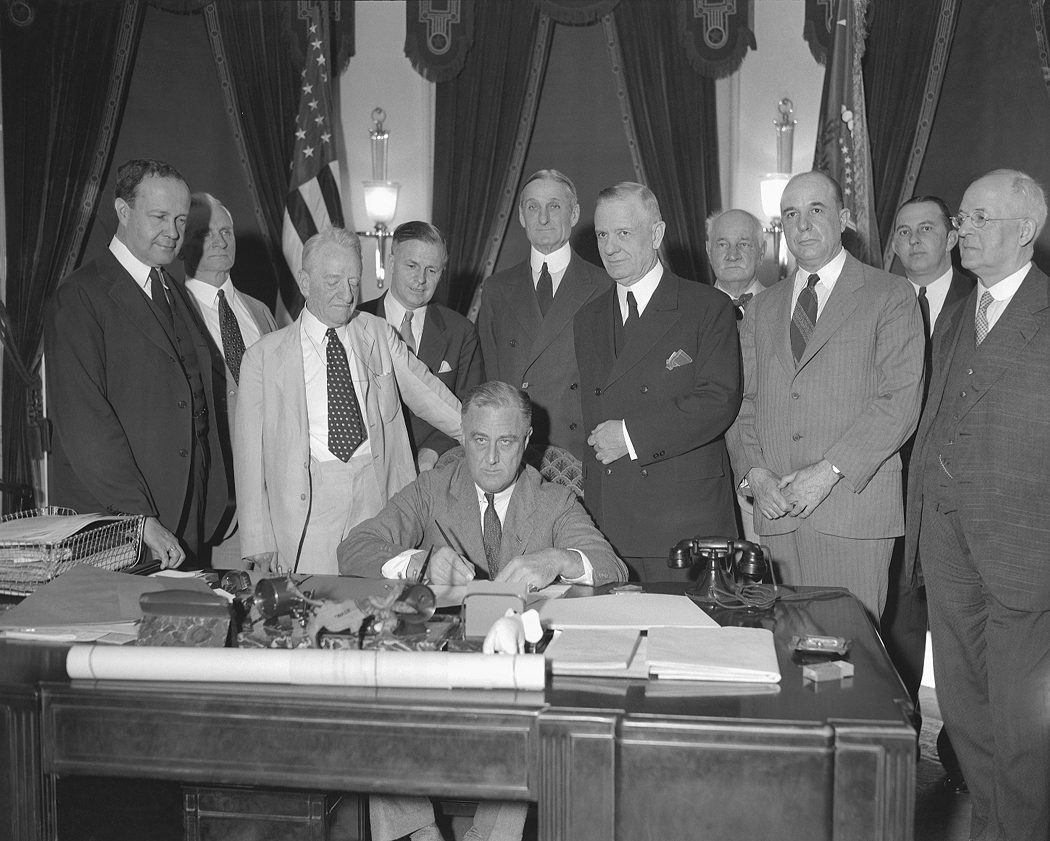
\includegraphics[width=1\textwidth]{GS1.png}
\end{figure}
\end{frame}







%---------------------------------------------------------------------

%-------------------------------------------------------
\begin{frame}
\frametitle{Banking Act of 1933}
At the time it was legislated, and for several decades thereafter, the
Banking Act of 1933 reflected in some measure a sound economic approach
to regulation in case of market failure:
\begin{itemize}
\item \textit{Identify the market failure}, or in other words, why the collective outcome of individual economic agents and institutions does not lead to
socially efficient outcomes, which in this case reflected the financial
fragility induced by depositor runs.
\item \textit{Address the market failure through a government intervention}, in this case by insuring retail depositors against losses.
\item \textit{Recognize and contain the direct costs of intervention, as well as the indirect costs due to moral hazard arising from the intervention}, by
charging banks up-front premiums for deposit insurance, restricting
them from riskier and more cyclical investment banking activities, and,
through subsequent enhancements, requiring that troubled banks face
a “prompt corrective action” that would bring about their orderly resolution at an early stage of their distress.
\end{itemize}




\end{frame}

%----------------------------------------------------------------------
%======================================================================




%Day 2 section 2




%======================================================================
%----------------------------------------------------------------------

% \begin{frame}
% \begin{center}
% Case study for Day 1 - but done on day 2: Separation of Commercial and Investment Banking: The Morgans vs. The Rockefellers	- General discuss the pro's and cons of the Glass Steagull Act. ESTI TO ADD SLIDES.
% \end{center}
% \end{frame}

% \begin{frame}
% \begin{center}
% Paper for day 2 (A): History of the US banking crisis of 1933 - %https://www.jstor.org/stable/2701075?seq=1#page_scan_tab_contents This can also be a case study then that students can do as well.
% There will also be another paper on day 2 -  Brunnermeier's paper "Deciphering the Liquidity Crunch of 2008" to be done after the financial crisis section?
% \end{center}
% \end{frame}


\begin{frame}
\begin{center}
Getting rid of Glass-Steagall
\end{center}
\end{frame}


%--------------------------------------------------------------------
\begin{frame}
\frametitle{Glass-Steagall recap}
Over time, the term Glass–Steagall Act came to be used most often to refer to four provisions of the 1933 Banking Act that separated commercial banking from investment banking.\\
\begin{itemize}
\item Glass-Steagall Act is a law that prevented banks from using depositors' funds for risky investments (stock market) \\$\Rightarrow$ Separated investment banking from retail banking
\item Institutions were given one year to decide whether they wanted to specialize in commercial or investment banking.
\item Glass-Steagall was enacted as an emergency response
\end{itemize}
\end{frame}

%---------------------------------------------------------------------
\begin{frame}
\frametitle{Glass-Steagall recap}
\begin{figure}
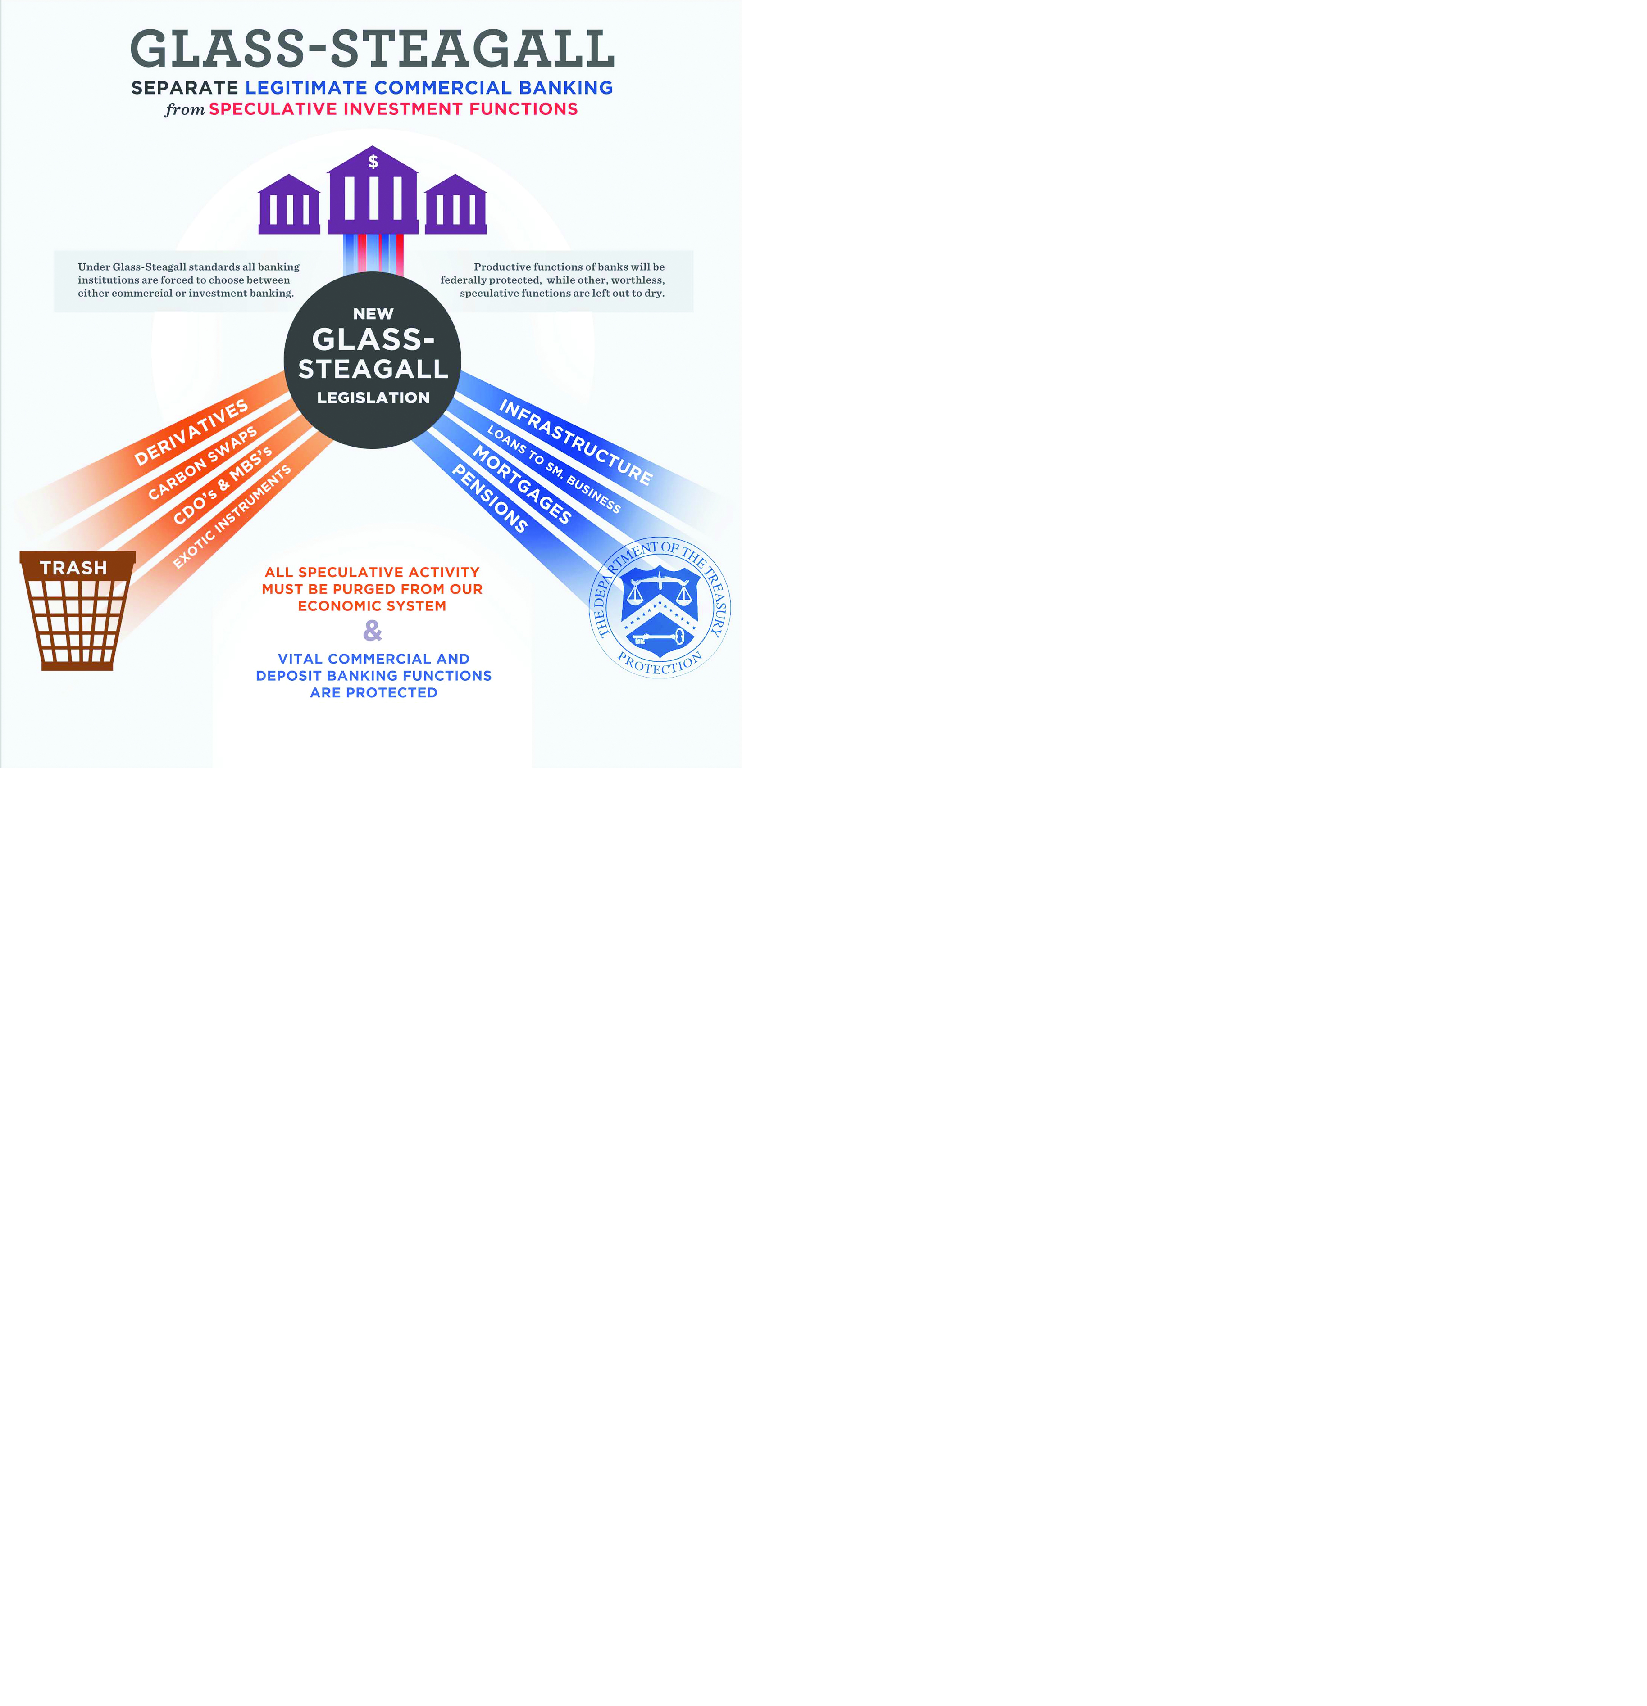
\includegraphics[width=1.5\textwidth]{GS3.png}
\end{figure}
\end{frame}

%---------------------------------------------------------------------
\begin{frame}
\frametitle{Justification of the rate ceilings - Regulation Q}
\begin{itemize}
\item \textbf{Shield bank profits by limiting the competition for
deposits} View: competition for deposits not only reduced bank profits by raising interest expenses, but also could cause banks to seek riskier investments and make high risk loans in order to cover the costs.
\item \textbf{Encourage country banks to lend more in their local communities} rather than hold balances with larger banks in financial centers.
\item \textbf{Deposit interest rate ceiling would compensate banks for the costs incurred by the newly introduced
deposit insurance premiums}
\item \textbf{Ceilings were extended to thrift institutions} such as
mutual savings banks, savings and loan associations in 1966 - policymakers believed that competition for deposits between commercial banks and thrifts as one of the reasons of the rise in residential mortgage interest rates and the subsequent slowdown in lending growth

\end{itemize}
\end{frame}

%-----------------------------------------------------------------
\begin{frame}
\begin{figure}
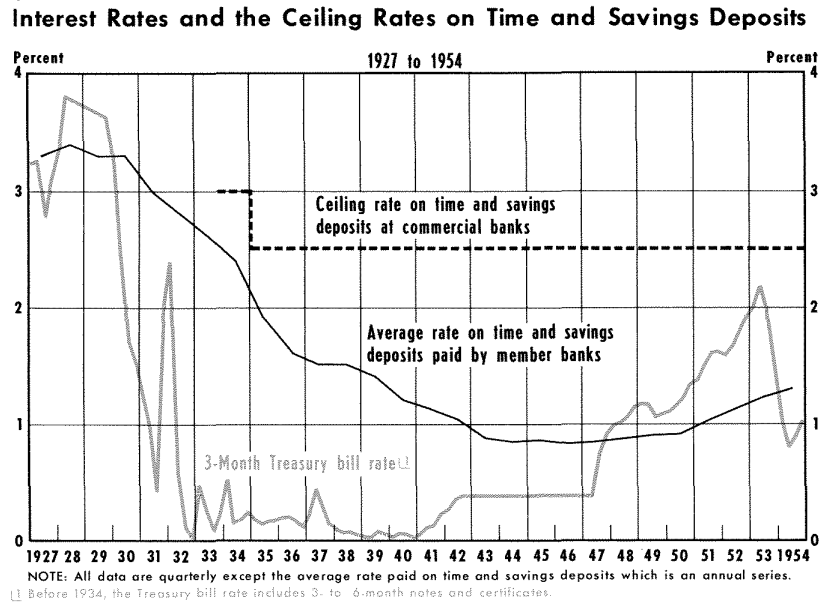
\includegraphics[width=\textwidth]{Interestceiling1.png}
\end{figure}
\tiny{Source: Gilbert, 1986}
\end{frame}
%---------------------------------------------------------------------------
\begin{frame}
\frametitle{Issues with Glass-Steagall}

\begin{itemize}
\item Limiting deposit interest rate competition through rate limitations
\item Restricting competition for deposits based on financial strength by insuring depositors
\item Critics argued that Regulation Q's limits on interest rates created the "disintermediation" that began in the 1960s
\item Allowed commercial banks to earn high profits until nonbanking companies found ways to offer substitutes for bank loans and deposits...
\item ... Over time, Regulation Q made bank deposits less attractive relative to other savings products and helped boost fund industry growth,
particularly, money market mutual funds.
\item $\Rightarrow$ the development of substitutes to bank deposits




\end{itemize}


\end{frame}
%---------------------------------------------------------------------
\begin{frame}
\begin{figure}
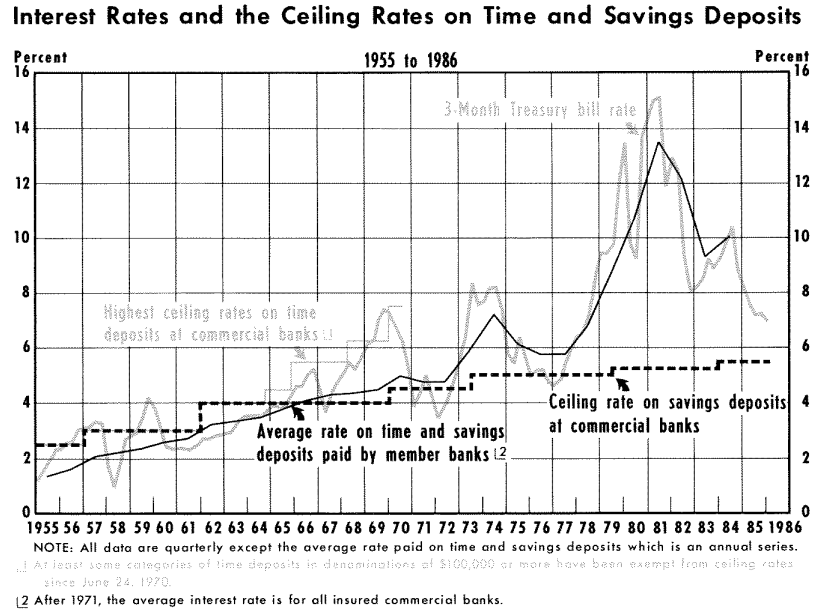
\includegraphics[width=\textwidth]{Interestceiling2.png}
\end{figure}
\tiny{Source: Gilbert, 1986}

\end{frame}



%---------------------------------------------------------------------
\begin{frame}
\frametitle{Deregulation}

\begin{itemize}
\item Monetary Control Act (MCA) of 1980 - established the Depository Institutions Deregulation Committee (DIDC), main duty - phase out the regulation over a period of 6 years. MCA contained several provisions relating to bank reserve and deposit requirements. It created the popular Negotiable Order of Withdrawal (NOW) accounts and also raised the amount of FDIC insurance protection from $\$$40,000 to $\$$100,000 per account.

\begin{itemize}
\item deregulation of interest rates paid by depository institutions such as banks
\item opened the Fed discount window
\item extended reserve requirements to all domestic banks
\end{itemize}


\item Glass-Steagall was repealed in 1999 by the Gramm-Leach-Bliley Act.
\end{itemize}


\end{frame}

%------------------------------------------------------------------
\begin{frame}
\frametitle{Bank disintermediation}
The term “banking disintermediation” refers to a situation
where
\begin{itemize}
\item banks no longer hold the loans they originated
on their balance sheets but sell them off;
\item borrowers go directly to the capital markets rather than to banks
to obtain a credit; or
\item savers invest directly in securities, such as government and private bonds, asset-backed securities, stocks, rather than leaving
their money in savings accounts on banks’ balance sheets
\end{itemize}

These trends began to emerge in the US in the 1980s-
1990s. However, there is no simple and univocal
explanation to the process of disintermediation. It has
resulted from a series of interdependent events,
regulatory changes, policy decisions, historic events,
macroeconomic conditions and cultural factors.
\end{frame}




%----------------------------------

\begin{frame}
\frametitle{A shift from banks tot non-banks}
\begin{itemize}
\item  In 1980, banks still held 60$\%$ of total debt instruments (loans and debt securities) held by the domestic financial sector... but
\item total non-bank lending significantly outpaced bank lending beginning in the 1990s



\end{itemize}
\end{frame}


\begin{frame}
\begin{figure}
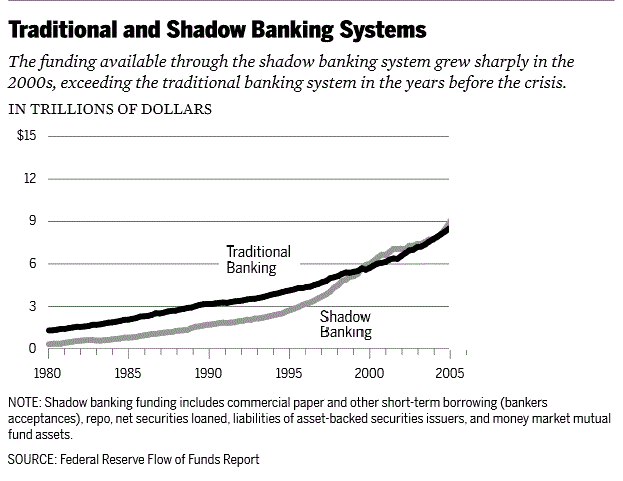
\includegraphics[width=1 \textwidth]{SB1.png}
\end{figure}
\end{frame}
%----------------------------------------------------------------

\begin{frame}
\frametitle{Federal guarantees in the mortgage market}
The rise of securitization, in the 1980s, was strongly supported by the introduction of federal guarantees in the mortgage market
\begin{itemize}
\item The US housing policy and particularly the introduction of
federal guarantees in mortgages markets helped transform
the funding structure of the US economy
\item The creation of GSEs planted the seeds for linking mortgage markets with broader capital markets...
\item by creating a strong secondary mortgage market for housing loans in order to  provide a stable source of funding for residential mortgages across the country (particularly for low- and moderate-income households)
\item  ‘originate to distribute’ model

\end{itemize}

\end{frame}

%--------------------------------------------------------------
%======================================================================
%----------------------------------------------------------------------
% ------------------------------------------------------------------

\begin{frame}
\begin{center}
\centering{\Large Day 2 session 3 - A short history of Basel I and II}
\end{center}
\end{frame}

\begin{frame}
\frametitle{Overview}
\begin{itemize}
\item When a poorly capitalized financial firm suffers asset losses, the firm falls into distress
\item Funding declines which means firms sells assets
\item If the firm that faces the loss is significant, it affects the market by a decline in the aggregate shortfall of capital
\item Systemic risk emerges and the financial system erodes
\item Capital can save the financial system
\item In response to the systemic effect of the failure of a relatively small German bank, Herstatt in 1974, Basel I was introduced
\item It formulates international standards for banking supervision
\end{itemize}
\end{frame}

\begin{frame}
\frametitle{Basel I}
Basel Capital Accord, the current international framework on capital adequacy, was adopted in 1988 by a group of central banks and other national supervisory authorities, working through the Basel Committee on Banking Supervision.
\begin{itemize}
\item objectives: promote soundness and  stability of the international banking system, provide equitable basis for international competition among banks
\item intended specifically for internationally active banks, but accord has been applied beyond largest institutions to cover most banks
\item Accord is a framework for measuring capital adequacy and a minimum standard to be achieved by international banks in adopting countries
\item Original framework $\rightarrow$ assessed capital mainly in relation to credit risk
\item Credit risk $\Rightarrow$ the risk of loss due to the failure of a counterparty to meet its obligations
\end{itemize}
\end{frame}

\begin{frame}
\frametitle{Basel I cont}
The first Basel Capital Accord was published in July 1988 and fully implemented in the US by the end of 1992.
\begin{itemize}
\item Basel I imposes a minimum ratio of capital to risk-weighted assets of $8$\%
%\item Basel II expands on Basel I's capital requirement rule and introduces internal risk assessment processes
%\item Basel III is implemented by the Dodd-Frank Wall-Street Reform and Consumer Protection Act
\end{itemize}
the Basel Capital Accord requires that a bank have available as ''regulatory capital'' (through combinations of equity, loan-loss reserves, subordinated debt, and other accepted instruments) at
least 8 percent of the value of its risk-weighted assets (loans and securities, for example) and asset equivalent off-balance-sheet exposures (such as loan commitments, standby letters of credit, and obligations on derivatives contracts).
\tiny{Source: https://www.federalreserve.gov/pubs/bulletin/2003/0903lead.pdf}
\end{frame}


\begin{frame}
\frametitle{Need for a new capital standard}
\begin{itemize}
\item Basel I, is widely viewed as having achieved its principal objectives of promoting financial stability and providing an equitable basis for competition among internationally active banks
\item also seen as having outlived its usefulness, at
least in relation to larger banking organizations
\item but there are clear shortcomings
\end{itemize}
\end{frame}


\begin{frame}
\frametitle{Shortcomings of Basel I}
\begin{itemize}
\item Too simple to address the activities of the most complex
banking organizations
\item  Specifies only 4 levels of risk as implemented in the US, even though loans assigned the same risk weight (for example, 100 percent for commercial loans) can vary greatly in credit quality
\item limited differentiation among degrees of risk $\rightarrow$ calculated capital ratios are often uninformative and may provide misleading information about a bank's capital adequacy relative to its risks
\item $\rightarrow$ creates incentives for banks to \textit{game} the system through regulatory capital arbitrage by selling, securitizing, or otherwise avoiding exposures for which the regulatory capital requirement is higher than the market requires and pursuing those for which the requirement is lower than the market would apply to that asset

\end{itemize}
\tiny{https://www.federalreserve.gov/pubs/bulletin/2003/0903lead.pdf}

\end{frame}

\begin{frame}
\frametitle{Towards Basel II}
For the larger banks, in short, Basel I capital ratios neither reflected risk adequately nor measure bank strength accurately
\begin{itemize}
\item Evolution of the Art of Risk Measurement and Management.
\begin{itemize}
\item Banks themselves led the development of new techniques to improve their risk management and internal economic capital measures in order to be more effective competitors and to control and manage their credit
losses.
\item But, clearly they can go considerably further
\end{itemize}
\item Continuing Concentration of the Banking Industry.
\begin{itemize}
\item Market pressures have led to consolidation in banking around the world.
\item US banking system part of this trend;
\item $\rightarrow$ became increasingly concentrated - small number of very large banks, operating across a wide range of product and
geographic markets
\item complex and sophisticated operations
\item these banks, with their scale and role in payment and settlement systems and in derivatives markets, have presented authorities with greater moral hazard
\end{itemize}
\end{itemize}

\tiny{Source: https://www.federalreserve.gov/pubs/bulletin/2003/0903lead.pdf}
\end{frame}


\begin{frame}
\frametitle{Basel II}
\begin{itemize}
\item Consultative paper in April 2003
\item focus: strengthening the regulatory capital framework for large, internationally active banking organizations through minimum capital requirements that are more sensitive to an institution's risk
profile and that reinforce incentives for strong risk management
\item proposed substitute for the current capital accord is more complex than Basel I
\end{itemize}

\end{frame}

\begin{frame}
\begin{figure}
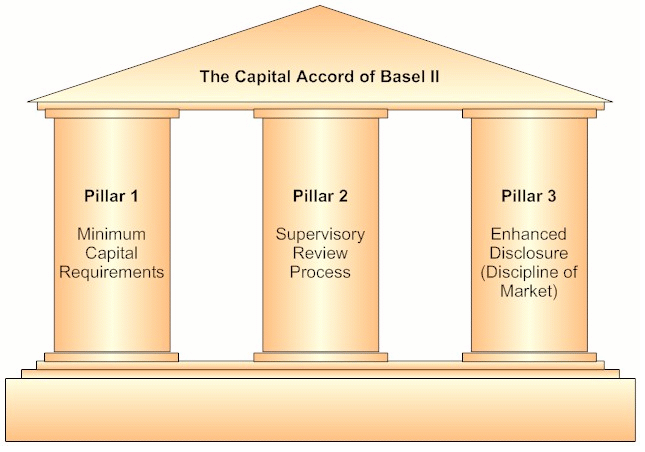
\includegraphics[width=1 \textwidth]{BaselII.png}
\end{figure}
\tiny{Source: IBM}
\end{frame}



\begin{frame}
\begin{center}
 Day 2 Session 4 \\
The Global Financial Crisis
\end{center}
\end{frame}


%--------------------------------------------------------------------
\begin{frame}
\begin{figure}

\includegraphics[]{Lehman.png}
\end{figure}
\end{frame}





\begin{frame}
\frametitle{Leading up to the crisis}
\begin{itemize}
\item Massive new inflows of capital into the US, mostly from oil-producing and Asian countries since the early 2000s
\item Increase in house prices in the US (also Spain,
Ireland, …)
\item Mid-2006: house prices begin to stagnate
\item February 2007: Prices of Credit Default Swaps for sub-prime
mortgages in the US collapse by 30 $\%$.
\item Mid-June 2007: Bear Stearns injects $\$$3.2 billion in two hedge funds in order to avoid their liquidation.
\item End July 2007: American Home Mortgage Investment Corp. ceases
interest payments, bankruptcy on 6 August.
\item 9 August: BNP Paribas suspends payouts for 3 investment funds
because of the impossibility to value underlying assets.
\end{itemize}
\tiny{Source: E von Thadden 2012}
\end{frame}


%---------------------------------------------------------------
\begin{frame}
\begin{itemize}
\item September – December: increasing write-downs on
mortgage backed securities
\item January 2008: Hypo Real Estate (Germany) acknowledges
temporary funding problems
\item March 5: Carlyle Capital (NY) bankrupt. Bear Stearns suffers major losses.
\item March 13: Bear Stearns obtains no more funding on the repo market
\item March 14-16: Federal Reserve Bank of New York brokers the acquisition of Bear Stearns by JP Morgan Chase for $\$$236 million, loan of $\$$30 billion to JP Morgan Chase.
\item September 15: Lehmann Brothers bankrupt with $\$$613 billion of debt, Merrill Lynch taken over by Bank of America.
\end{itemize}
\tiny{Source: E von Thadden 2012}
\end{frame}

%------------------------------------------------------------
\begin{frame}
\frametitle{Causes of the crisis}
\begin{itemize}
\item Excessive US mortgage lending
\item Excessive securitization
\item Failure of bank risk models
\item Inadequate corporate governance of banks
\item Faulty financial regulation: - systemic risk, shadow banking?
\item Systemically Important Financial Intermediaries
\item Break-down of interbank market
\item Biased rating agencies
\item Savings glut (China, Middle East, Germany, …)
\item Real-estate price bubble (US, UK, Spain, …)
\item US Federal Reserve interest rate policy
\end{itemize}

\tiny{Source: E von Thadden 2012}

\end{frame}

%---------------------------------------------------------------

\begin{frame}
\begin{figure}
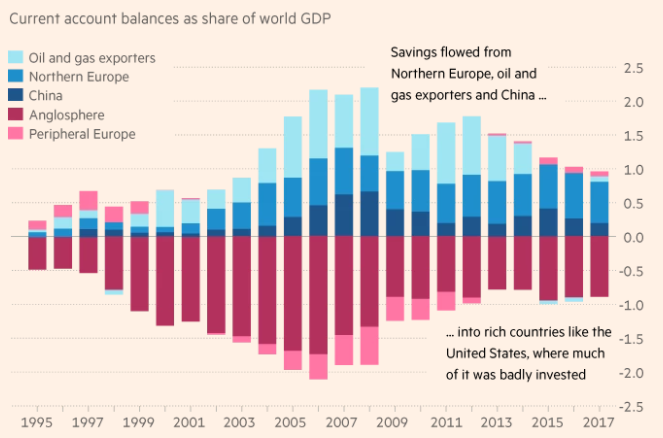
\includegraphics[width=1\textwidth]{SavingsGlut.png}
\end{figure}
\tiny{Source: Financial Times. https://www.ft.com/content/56d25a52-7df5-11e7-9108-edda0bcbc928}
\end{frame}
%---------------------------------------------------------------

\begin{frame}
\begin{figure}
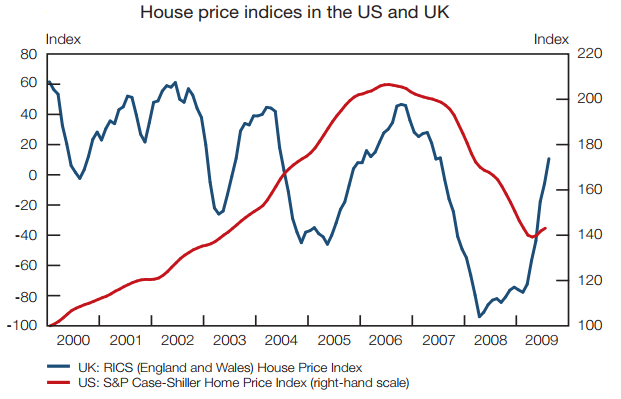
\includegraphics[width=1\textwidth]{HPUS.png}
\end{figure}
\tiny{Source: Financial Stability Review, Sept 2009, SARB}
\end{frame}


\begin{frame}
\begin{figure}
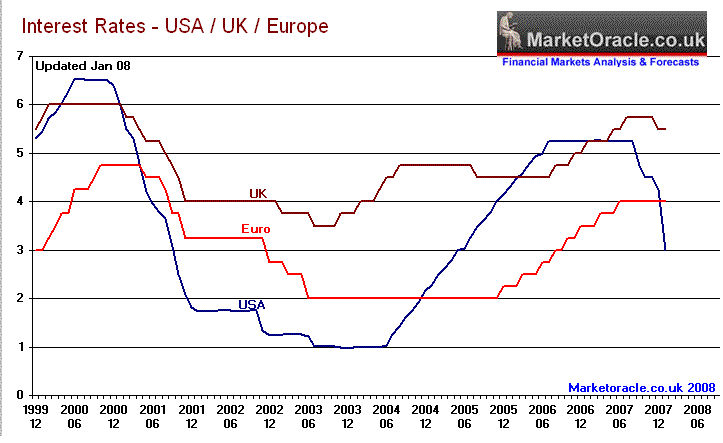
\includegraphics[width=1\textwidth]{Intrate.png}
\end{figure}
\tiny{Source: Market Oracle.co.uk}
\end{frame}

\begin{frame}
\frametitle{NINJA loans}
\begin{figure}

\includegraphics[width=1 \textwidth]{Ninja.png}
\end{figure}
Generally lenders require the borrower to show a stable stream of income or sufficient collateral. A NINJA loan ignores the verification process

\end{frame}

\begin{frame}
\frametitle{NINJA = No Income, No Job or Assets}
\begin{itemize}
\item sub-prime mortgages were mis-sold in their millions by lenders desperate to feed the pipeline for securitising, or packaging up, these loans by investment banks
\item Research by the industry's regulator, the Financial Services Authority:
\begin{itemize}
\item poor practices by mortgage brokers (account for more than 60 per cent of all mortgages sold) and lenders
\item in half the cases it investigated customers had self-certified their income
\item significant numbers of consumers' had been advised to remortgage - thus incur additional charges, without the adviser being able to demonstrate that this was beneficial to the customer
\item in a third of cases the intermediaries failed to assess properly the borrower's ability to afford the mortgages
\item Lenders had inadequate lending standards which they often failed to apply properly
\end{itemize}

\end{itemize}

\end{frame}
\begin{frame}
\begin{itemize}
\item Basel I imposes a minimum ratio of capital to risk-weighted assets of $8$\%
\item Basel II expands on Basel I's capital requirement rule and introduces internal risk assessment processes
\item Basel III is implemented by the Dodd-Frank Wall-Street Reform and Consumer Protection Act
\end{itemize}
\end{frame}


\begin{frame}
The Basel process focuses on capital requirements and ignores crucial market and regulation failures of the financial system as follows:
\begin{enumerate}
\item Focus on the risk of individual institution, not the system
\item Runs into shadow banking issues because of this focus
\item No recognition of the role of government
\end{enumerate}
~\\
\begin{itemize}
\item Even with the tightening of off-balance-sheet financing in Basel III , the focus is not to measure quantities that reflect systemic risk
\item There are two types of risk that causes a firm to fail:
	\begin{enumerate}
		\item Solvency risk: Market value of a firm's assets falls below its obligations
		\item Liquidity risk: Firms cannot convert assets into cash to pay off its obligations because asset markets have become illiquid
	\end{enumerate}
\item These risks spread quickly through fire sales, counterparty risk or contagious runs
\end{itemize}
\end{frame}

\begin{frame}
\frametitle{Financial crisis of 2007 to 2009}
\begin{itemize}
\item During this time banks and other intermediaries shift risks by exploiting loopholes in regulatory capital requirements
\item The following table shows the 12 largest write-downs (credit losses) of US financial institutions from June 2007 till March 2010
\end{itemize}
\end{frame}

\begin{frame}
\begin{figure}
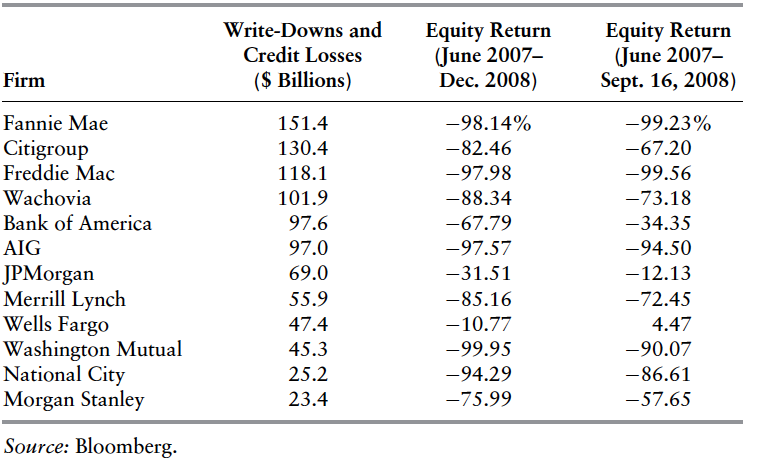
\includegraphics[width=\textwidth]{table6_1.png}
\end{figure}
\end{frame}

\begin{frame}
\begin{itemize}
\item The top 6 firms combined for a total of 696 billion dollars in losses
\item The last column shows market the value of the firms, 6 firms dropped in market value, averaging $-88.71$\% from June 2007 till December 2008
\item It also shows that under the Basel core capital requirement, the top 20 US banks looked safe, averaging a ration of $11.70$\%
\item Reasons this happened:
\begin{enumerate}
\item LCFI's took their leveraged bets and used it to engage in \mcdr{regulatory arbitrage}
\item They funded portfolios of risky loans via off-balance-sheet vehicles
\item Loans were guaranteed by sponsoring LCFI's through liquidity enhancements that have lower requirements by the Basel Accord
\item They made purchases of AAA-rated tranches of non-prime securities which implies low credit risk and zero liquidity and funding risk
\item Full capital relief on AAA-rated tranches
\end{enumerate}
\end{itemize}
\end{frame}

\begin{frame}
\begin{itemize}
\item The solution is for banks to provide their counterparties with guarantees on the underlying credit
\item The guarantees have two effects:
\begin{enumerate}
\item Guaranteeing the risk to bank counterparties leads to move assets off the banks balance sheets
\item Ensures highest ratings for off-balance-sheet vehicles from rating agencies
\end{enumerate}

\end{itemize}
\end{frame}

\begin{frame}
\begin{itemize}
\item Acharya, Schnabl and Suarez (2009) documented an increase in the ABCP (asset backed commercial paper) from 600 million dollars in 2004 to 1.2 trillion dollars in the second quarter of 2007
\item Collapse occurred: cost of issuing ABCP rose from 15 basis points over the federal funds rate to over 100 basis points
\item Banks had to return the loans to their balance sheets
\item Of the 1.2 trillion dollars in asset-based securitized vehicles, 4.3 \% of the loss was structured to remain with investors
\item The remaining loss wiped out significant portions of bank capital and threatened banks solvency
\item Another method would be for banks to make loans and move them from its balance sheet by securitizing them
\end{itemize}
\end{frame}
%
%==================================================================================
\begin{frame}
\begin{center}
{\Large Day 2 Session 5 - Interlude: Regulatory Arbitrage}
\end{center}
\end{frame}

\begin{frame}
	\frametitle{Acharya, Schnabl, and Suarez (2013, JFE) "Securitization Without Risk Transfer"}
    \begin{figure}
    	\begin{center}
    	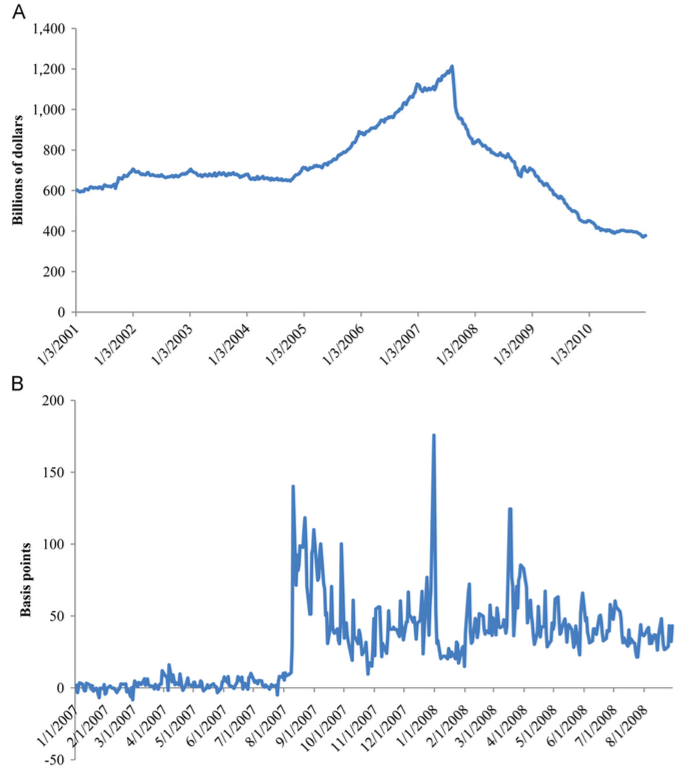
\includegraphics[width=0.6\textwidth]{Figures/ASS2013_Figure1.png}
        \end{center}
    \end{figure}
\end{frame}

\begin{frame}
	\frametitle{Acharya, Schnabl, and Suarez (2013, JFE) "Securitization Without Risk Transfer"}
    \begin{figure}
    	\begin{center}
    	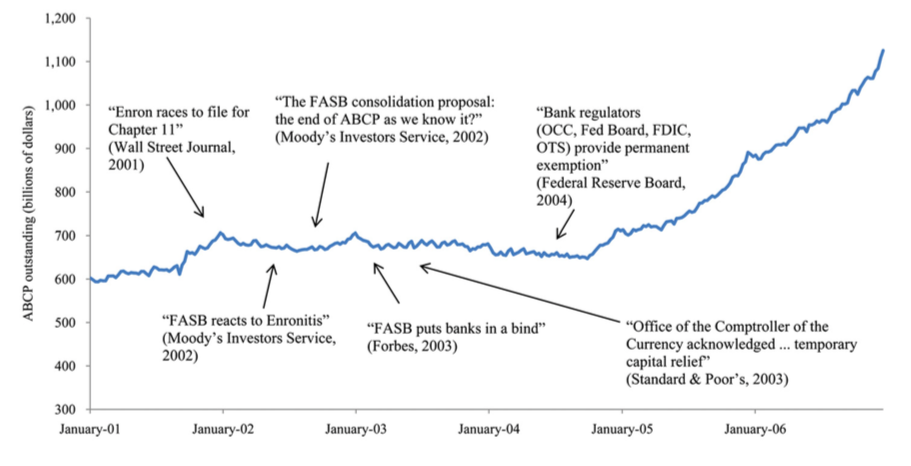
\includegraphics[width=\textwidth]{Figures/ASS2013_Figure2.png}
        \end{center}
    \end{figure}
\end{frame}

\begin{frame}
	\frametitle{Acharya, Schnabl, and Suarez (2013, JFE) "Securitization Without Risk Transfer"}
    \begin{figure}
    	\begin{center}
    	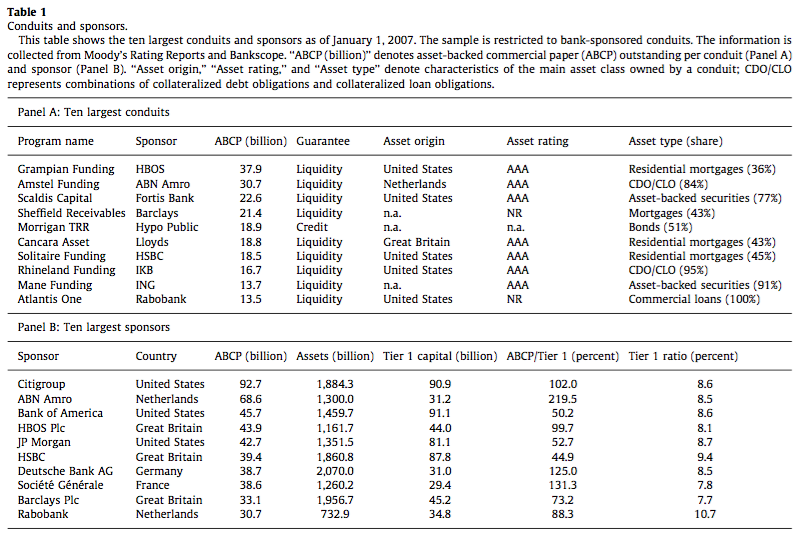
\includegraphics[width=0.8\textwidth]{Figures/ASS2013_Table1.png}
        \end{center}
    \end{figure}
\end{frame}

\begin{frame}
	\frametitle{Acharya, Schnabl, and Suarez (2013, JFE) "Securitization Without Risk Transfer"}
    \begin{figure}
    	\begin{center}
    	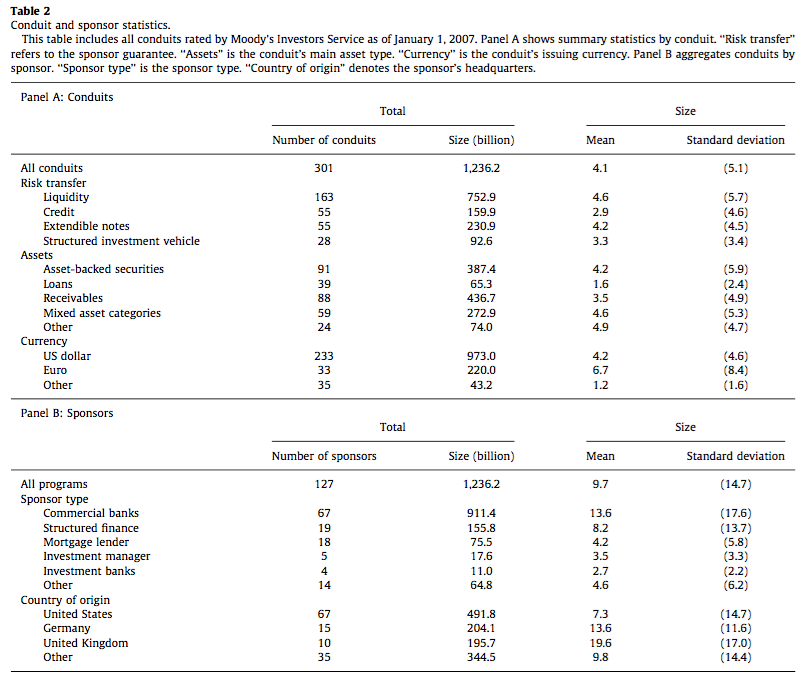
\includegraphics[width=0.8\textwidth]{Figures/ASS2013_Table2.png}
        \end{center}
    \end{figure}
\end{frame}

\begin{frame}
	\frametitle{Acharya, Schnabl, and Suarez (2013, JFE) "Securitization Without Risk Transfer"}
    ABCP outstanding by sponsor and guarantee. A - Commercial banks, B - structured finance companies, C - Mortgage originators
    \begin{figure}
    	\begin{minipage}{0.33\textwidth}
	    	\begin{center}
	    		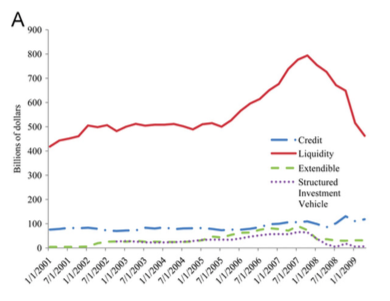
\includegraphics[width=\textwidth]{Figures/ASS2013_Figure3-A.png}
        	\end{center}
         \end{minipage}\begin{minipage}{0.33\textwidth}
	    	\begin{center}
	    		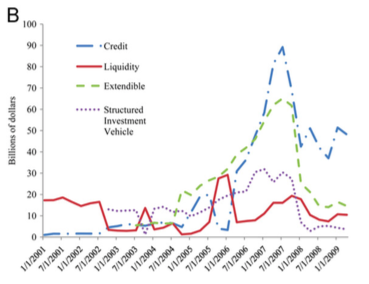
\includegraphics[width=\textwidth]{Figures/ASS2013_Figure3-B.png}
        	\end{center}
         \end{minipage}\begin{minipage}{0.33\textwidth}
	    	\begin{center}
	    		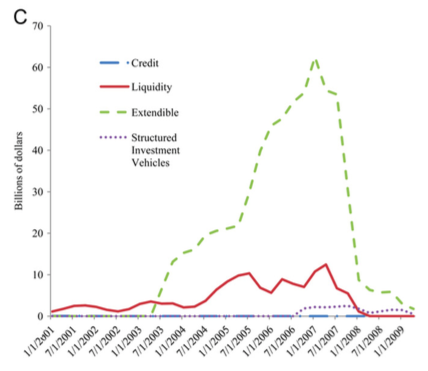
\includegraphics[width=\textwidth]{Figures/ASS2013_Figure3-C.png}
        	\end{center}
         \end{minipage}
    \end{figure}
\end{frame}

\begin{frame}
	\frametitle{Acharya, Schnabl, and Suarez (2013, JFE) "Securitization Without Risk Transfer"}
    \begin{figure}
    	\begin{center}
    	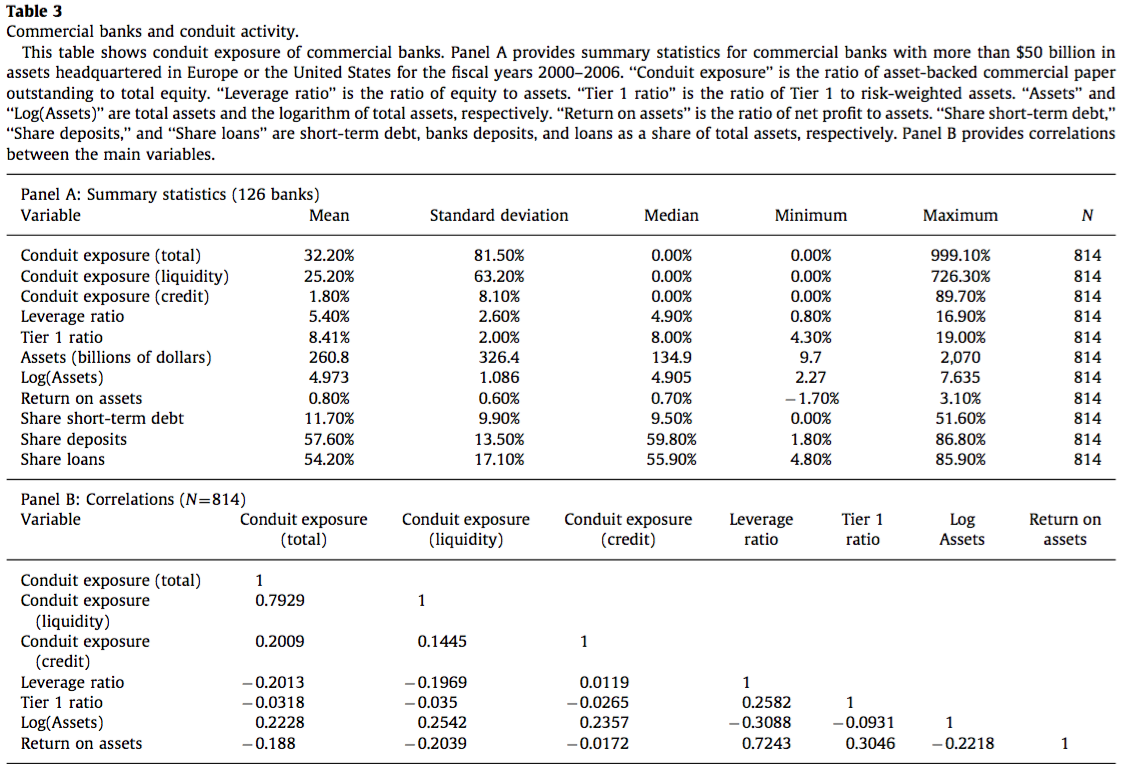
\includegraphics[width=0.8\textwidth]{Figures/ASS2013_Table3.png}
        \end{center}
    \end{figure}
\end{frame}

\begin{frame}
	\frametitle{Acharya, Schnabl, and Suarez (2013, JFE) "Securitization Without Risk Transfer"}
    \begin{figure}
    	\begin{center}
    	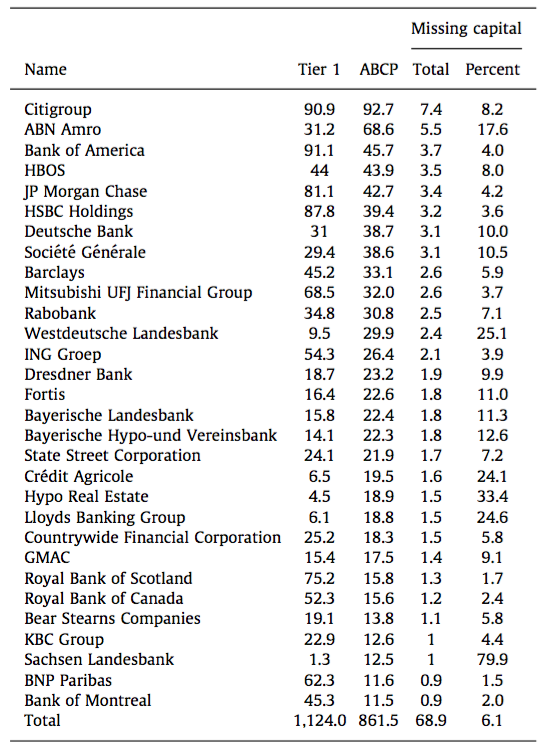
\includegraphics[width=0.5\textwidth]{Figures/ASS2013_Table10.png}
        \end{center}
    \end{figure}
\end{frame}

\begin{frame}
	\begin{center}
    	{\Large Day 2 Session 6 - The global financial crisis and the response in the US}
    \end{center}
\end{frame}



\begin{frame}
\begin{itemize}
\item However, banks then reinvest in AAA-rated tranches of the same securitized products it had created
\item Due to the AAA-ratings, securities had a significantly lower capital requirement under Basel III
\item Basel Accord weighted the risk of AAA-rated securities at less than half of the risk of ordinary commercial or mortgage loans
\item This leads to lower capital reserves for them
\item 2004: SEC allowed American investment banks the ability to employ internal models
\item These allow for banks to assess credit risk and the corresponding capital change
\item Debt-to-equity ratio: Moves from 22:1 to 33:1 over 3 years
\end{itemize}
\end{frame}

\begin{frame}
\begin{itemize}\itemsep10pt
\item Banks, GSE's and broker dealers in 2007 held 789 billion dollars of AAA-rated collateralized debt obligation (CDO) tranches
\item These are backed by non-prime loans
\item Majority of the subordinated tranches of the CDO's were also held by banks
\item They collectively held 320 billion dollars out of the 476 billion dollars of total outstanding tranches
\end{itemize}
\end{frame}

\begin{frame}
\frametitle{US response to Lehman collapse and the subsequent crisis}
\framebox{Troubled Asset Relief Program (TARP)}\hfill \break
\begin{itemize}
\item The Emergency Economic Stabilization Act of 2008 (EESA) created the TARP program
\item signed into law by President George W. Bush on 3 October 2008
\item TARP program originally authorized expenditures of $\$$700 billion (In 2010 amount was reduced by Dodd-Frank Wall Street Reform and Consumer Protection Act)
\item allows the Treasury to purchase illiquid, difficult-to-value assets from banks and other financial institutions
\item TARP does not allow banks to recoup losses already incurred on troubled assets
\item (EESA) requires financial institutions selling assets to TARP to issue equity warrants, equity or senior debt securities (for non-publicly listed companies) to the Treasury
\end{itemize}
\end{frame}

\begin{frame}
\framebox{Public-Private Investment Program (P-PIP)}\hfill \break
\frametitle{US response to Lehman collapse and the subsequent crisis}
\begin{itemize}
\item buy toxic assets from banks' balance sheets
\item P-PIP has two primary programs
\begin{itemize}
\item Legacy Loans Program - attempt to buy residential loans from bank's balance sheets: Federal Deposit Insurance Corporation (FDIC) will provide non-recourse loan guarantees for up to 85 percent of the purchase price of legacy loans
\item Legacy securities program -  buy residential mortgage backed securities (RMBS) that were originally rated AAA and commercial mortgage-backed securities (CMBS) and asset-backed securities (ABS) which are rated AAA. The funds will come in many instances in equal parts from the U.S. Treasury's TARP monies, private investors, and from loans from the Federal Reserve's Term Asset-Backed Securities Loan Facility (TALF).
\end{itemize}
\end{itemize}
\end{frame}



\begin{frame}
Financial Crisis timeline
\begin{figure}
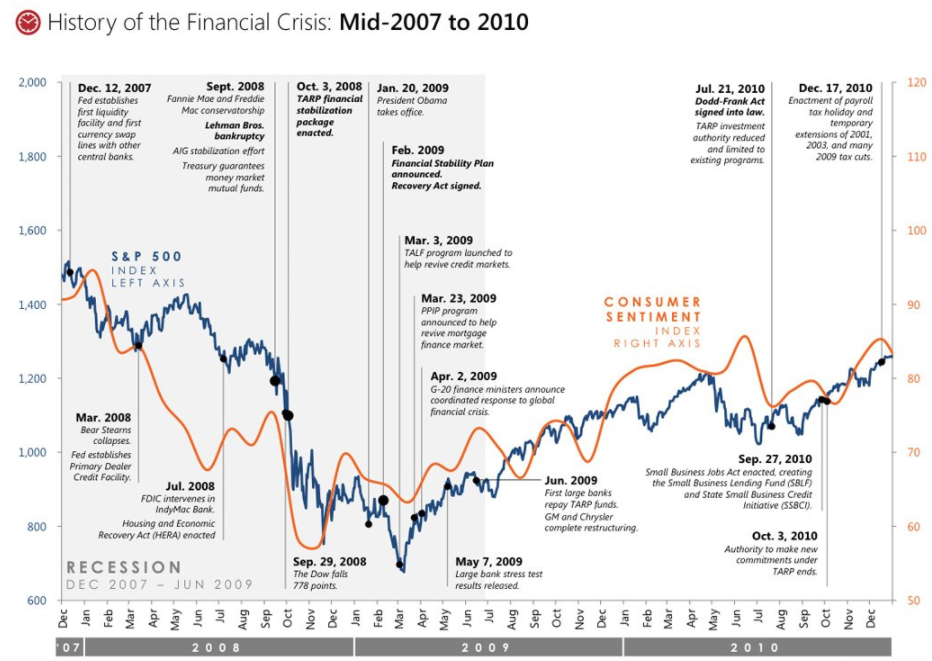
\includegraphics[width=1\textwidth]{GFC1.png}
\end{figure}
\tiny{Source:http://www.businessinsider.com/chart-financial-crisis-2013-9}
\end{frame}


\begin{frame}
\begin{center}
Day 3 Session 1 - The global financial crisis not just in the US - Focus on Iceland
\end{center}
\end{frame}

\begin{frame}
\begin{figure}
\centering
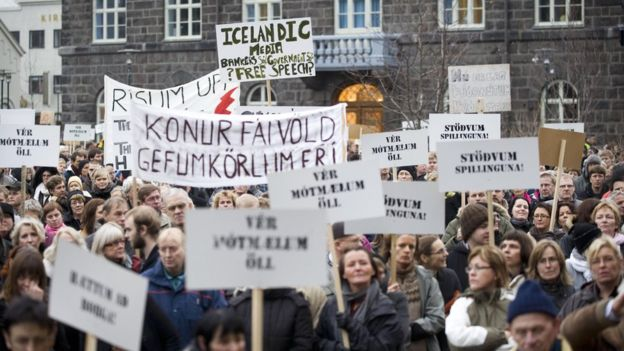
\includegraphics[width=\textwidth]{Iceland1.png}
\end{figure}
% \tiny{source: }
\end{frame}



\begin{frame}
\frametitle{Iceland Financial Crisis - Regulatory environment}
\begin{itemize}
\item Banks deregulated in 2001 - set stage for banks to upload debts when foreign companies were accumulated
\item Three big banks -  Landsbanki, Glitnir and Kaupthing
\item rapid growth facilitated by Iceland’s membership in the European Economic Area (EEA) - created regulatory framework rooted in the directives adopted by the European Union
\item = operating licenses granted to Icelandic financial companies extended not only to Iceland but to all other EEA states
\item Icelandic Financial Supervisory Authority based its operations
on European law, regulations, and procedures, and was given good marks by rating agencies and the International Monetary Fund.

\end{itemize}

\end{frame}

\begin{frame}
\frametitle{Iceland Financial Crisis - global financial markets}
\begin{itemize}
\item supply of credit was virtually inexhaustible
\item interest rates lower than they had been in a hundred years
\item financial markets - search for yield \\
$\rightarrow$ Bonds issued by Iceland's banks (welcome addition to popular structured securities)
\item Rating agencies - favourable credit ratings for bonds
\item banks became a vital link in the national economy
\end{itemize}
\end{frame}

\begin{frame}
\frametitle{Iceland - Rising debt}
\begin{itemize}
\item 15 percent interest rates - attract deposits especially from the Netherlands and the UK
\item Iceland's currency, the krona, became a major trading currency - value high
\item Banks' balance increase: cheap foreign financing allowed banking sector to increase assets from 100 to almost 900 percent of GDP between 2004 and end-2007
\item Households also increase debt
\item Higher demand = higher inflation = interest rates kept high
\end{itemize}
\end{frame}

\begin{frame}
\frametitle{Iceland - something is not right..}
\begin{itemize}
\item banks attracted international attention late in 2005 and early in 2006
\item  received more probing and critical coverage by the media, including scrutiny of growth rate, risk appetite, low deposit ratio's, lack of transparency etc.
\item  CDS spreads began rising toward the end of 2005
\item   February 2006 - Iceland’s Prime Ministry, Ministry of Finance, Ministry of Business Affairs, Financial Supervisory Authority, and Central Bank concluded a collaboration agreement centering on financial stability and contingency measures
\item government established an advisory group on basis of this agreement
\end{itemize}
\end{frame}

\begin{frame}
\frametitle{Banks' response to criticism}
\begin{itemize}
\item greatly enhanced their information disclosure
\item sought to reduce cross-ownership,
\item improve liquidity position and capital ratios,
\item took the first steps toward increasing the share of deposits on balance sheets, increased presence in retail deposit market abroad
\item Sought out new credit markets - including the US
\end{itemize}
Because of this, the Icelandic banks were perhaps better prepared than they would otherwise have been for the sudden changes that took place in the global financial markets in mid-2007
\\
\tiny{Source: http://www.bis.org/review/r090226d.pdf}
\end{frame}

\begin{frame}
\frametitle{Iceland - Yay for deposits (!?)}
\begin{itemize}
\item Sharp increase in risk aversion following developments in global financial markets
\item Credit supply shrinks
\item CDS spreads increase, also for Icelandic banks
\item Banks still confident - some leaders said \textit{easy to fund all  outstanding bonds and other debt for the coming years through deposit business in Europe}
\end{itemize}
\end{frame}

\begin{frame}
\frametitle{But..growing opposition to the Icelandic banks’
accumulation of deposits}
Why?
\begin{itemize}
\item banks in those same parts of Europe felt the pressure of the sudden competition and communicated their concerns to their authorities
\item accumulation of deposits in foreign subsidiaries increased the potential obligations of the deposit insurance schemes in the countries of operation
\item concerns that the relatively high interest rates offered by the Icelandic banks might reflect underlying weakness
\item concern about the Icelandic deposit insurance scheme with respect to deposits in foreign bank branches
\end{itemize}
\end{frame}

\begin{frame}
\frametitle{The Central Bank of Iceland}
\begin{itemize}
\item said that banks’ foreign deposits should be held in subsidiaries rather than branches - i.e. Landsbanki’s deposit business in London should be transferred to a subsidiary of the bank.
\item Preparation for the transfer began in early 2008
\item Central bank thought the process had started, but by July it had not - the central bank did not have the power to force changes or make demands.
\item Moreover - other Icelandic authorities also had limited legal power in this respect under the legislation then in force which was and is based on EU Directives.
\item Central bank kept close watch on the liquidity of the Icelandic banks throughout 2008
\item  tracked the banks’ liquidity virtually on a daily basis and kept abreast of their refinancing efforts and asset sales

\end{itemize}
\end{frame}


\begin{frame}
\frametitle{Glitnir}
\begin{itemize}
\item Glitnir, had a large foreign loan payment coming up in mid-October
\item Glitnir not active in creating retail deposit market abroad
\item increased liquidity by selling assets
\item mid-Sept: Meeting with central bank - Prospects for funding the October payment were good
\item \textbf{LEHMAN BROTHERS COLLAPSE}
\item $\Rightarrow$  virtually completed sale of Glitnir assets did not materialise
\end{itemize}
\end{frame}

\begin{frame}
\frametitle{Central bank assistance required}
\begin{itemize}
\item unsuccessful to sell assets
\item unable to renew a bank loan
\item $\rightarrow$Glitnir turned to the Central Bank for assistance
\item Ultimately, the Government decided that the Treasury should acquire a majority holding in Glitnir
\item before that could be finalised, the bank collapsed
\end{itemize}


\end{frame}


\begin{frame}
\frametitle{Landsbanki}
\begin{itemize}
\item  substantial pressure on Landsbanki’s deposit accounts in
London in early October
\item  British Financial Services Authority (FSA) steadily tightened the demands it made on the bank
\item Landsbanki’s liquidity difficulties became insurmountable, and it was clear that rescuing the bank would not represent prudent use of the Central Bank’s foreign exchange reserves - amounts were too large

\end{itemize}
\end{frame}

\begin{frame}
\frametitle{The last big bank standing - Kaupthing}
\begin{itemize}
\item In view of the prospects for Kaupthing’s liquidity, the bank was deemed likely to survive the storm
\item thus central bank, after consultation with government, granted the bank a collateralized 4-day loan that was expected to suffice
\item but FSA took action against the Kaupthing subsidiary
\end{itemize}
\end{frame}

\begin{frame}
\frametitle{Banking crisis}
\begin{itemize}
\item three leading commercial banks, representing about 85 percent of total banking assets collapsed - within a week
\item Icelandic Financial Supervisory Authority took over their operations on the basis of newly adopted legislation, and they were divided into two entities, the new banks and the old
\item The new banks, owned by the government, took over domestic banking activities
\item foreign operations remained within the old banks, which have been granted a moratorium on payment.
\item government’s response in October was guided by the overriding aim of guaranteeing continued domestic banking operations and domestic and cross-border payment intermediation under extraordinarily difficult circumstances.

\end{itemize}
\end{frame}

\begin{frame}
\begin{itemize}
\item The Central Bank of Iceland expanded its liquidity facilities, as did its foreign counterparts.
\item Iceland’s banks obtained funding both from their own Central Bank \item also through their foreign subsidiaries, from the ECB (in euros)
\item the Central Bank of Iceland could not provide liquidity in currencies other than the Icelandic króna
\item Banks became heavily dependent on ready access to liquidity facilities.
\item Icelandic government negotiated a Stand-By Facility
from the International Monetary Fund on basis of economic programme
\item Focussed on three objective
\begin{itemize}
\item stabilise the foreign exchange market and provide support for
the appreciation of the króna from its recent exceptionally low levels; \item formulate fiscal policy for 2009 and beyond aimed at establishing a sustainable level of debt;
\item restructure  banking system in a transparent manner consistent with internationally recognised practice.
\end{itemize}
\end{itemize}
\tiny{Source: http://www.bis.org/review/r090226d.pdf}
\end{frame}



% ------------------------------------------------------------------

\begin{frame}
\begin{figure}
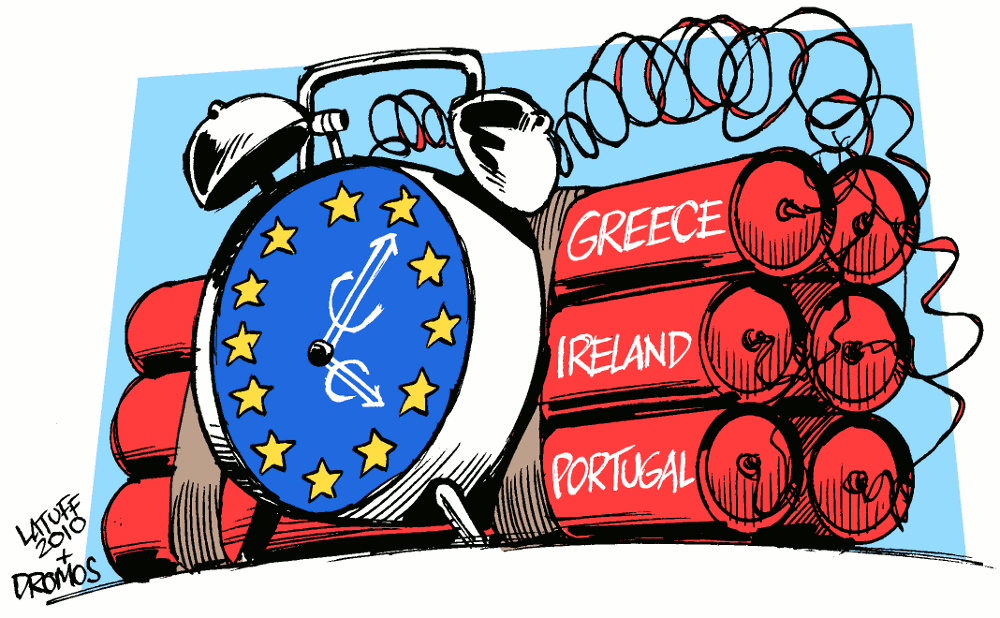
\includegraphics[width=1 \textwidth]{Europe1.png}
\end{figure}
\end{frame}

\begin{frame}
\begin{figure}
\frametitle{Day 3 Session2: Global financial crisis spillovers}
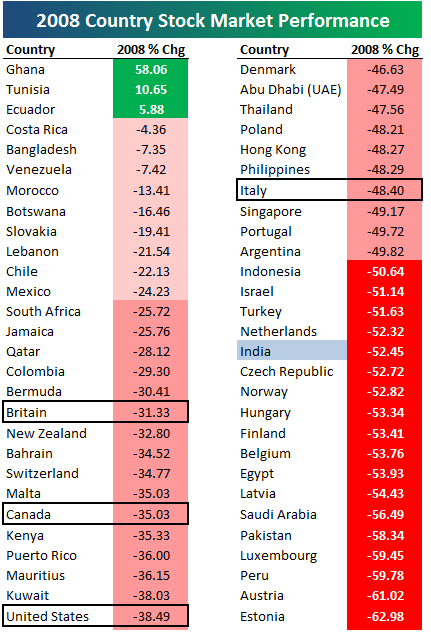
\includegraphics[width=0.5\textwidth]{Stockmarket2008.png}
\end{figure}
\tiny{Source: Economic Edge: 2008}
\end{frame}

\begin{frame}
\frametitle{Spillovers - European Sovereign Debt crisis}
\begin{itemize}
\item Starting in October 2008, European governments bailed out or guaranteed the debt of their banking system
\item Total amount of state aid (guarantees, liquidity measures, bank recapitalizations, impaired assets) 10/2008 – 10/2011: 37 per cent of GDP

\end{itemize}
\end{frame}

\begin{frame}
\frametitle{Background - The start of the European Sovereign Debt crisis}
\begin{itemize}
\item The euro was established in Maastricht by the European Union (EU) in 1992
\item 1999 currency comes into existence, notes and coin introduced in 2002
\item December 2008, EU leaders agree on a 200bn-euro stimulus plan to help boost European growth following the global financial crisis
\item 2009 EU orders France, Spain, the Irish Republic and Greece to reduce their budget deficits
\item Collapse of Iceland's banking system seen to have spread to Greece, Ireland and Portugal in 2009
\item December 2009 - Greece admits that its debts have reached 300bn euros - the highest in modern history.
\item Greece is burdened with debt amounting to 113$\%$ of GDP - nearly double the eurozone limit of 60$\%$.
\item Ratings agencies start to downgrade Greek bank and government debt.
\end{itemize}
\tiny{Source:http://www.bbc.com/news/business-13856580}
\end{frame}

\begin{frame}
\frametitle{Concerns over sovereign debt increases}
\begin{itemize}
\item In January 2010, an EU report condemns "severe irregularities" in Greek accounting procedures. Greece's budget deficit in 2009 is revised upwards to 12.7$\%$, from 3.7$\%$, x4 the maximum allowed by EU rules.
\item February 2010 Greece unveils a series of austerity measures aimed at curbing the deficit
\item Concern starts to build about all the heavily indebted countries in Europe - Portugal, Ireland, Greece and Spain.
\item The austerity plans in Greece spark strikes and riots in the streets
\item The eurozone and IMF agree a safety net of 22bn euros to help Greece - but no loans
\item eurozone countries agree to provide up to 30bn euros in emergency loans
\item EU announces that the Greek deficit is even worse than thought after reviewing its accounts - 13.6$\%$ of GDP, not 12.7$\%$.
\end{itemize}
\tiny{Source:http://www.bbc.com/news/business-13856580}
\end{frame}

\begin{frame}
\frametitle{Bailout package Greece and Ireland}
\begin{itemize}
\item May 2010 - eurozone members and the IMF agree a 110bn-euro bailout package to rescue Greece
\item Euro continue to depreciate
\item other EU member state debt starts to come under scrutiny, starting with the Republic of Ireland
\item EU and IMF agree to a bailout package to the Irish Republic totalling 85bn euros. The Irish Republic soon passes the toughest budget in the country's history
\item Amid growing speculation, the EU denies that Portugal will be next for a bailout
\end{itemize}
\tiny{Source:http://www.bbc.com/news/business-13856580}
\end{frame}


% \begin{frame}
% \begin{center}
% The Irish case: I think this should be a homework assignment or the case study - - how is Ireland different from Iceland response. What do you think?
% \end{center}

% \end{frame}



\begin{frame}
\frametitle{European Sovereign Debt crisis - Portugal and Greece again}
\begin{itemize}
\item  February 2010, eurozone finance ministers set up a permanent bailout fund, called the European Stability Mechanism, worth about 500bn euros
\item April 2010 - Portugal admits it cannot deal with its finances itself and asks the EU for help
\item May, the eurozone and the IMF approve a 78bn-euro bailout for Portugal
\item June 2010, eurozone ministers say Greece must impose new austerity measures before it gets the next tranche of its loan, without which the country will probably default on its enormous debts
\item July 2010, the Greek parliament votes in favour of a fresh round of drastic austerity measures, the EU approves the latest tranche of the Greek loan, worth 12bn euros
\item second bailout for Greece is agreed - 109bn-euro package
\item August - is crisis spreading beyond periphery?
\item yields on government bonds from Spain and Italy rise sharply, the ECB says it will buy Italian and Spanish government bonds
\end{itemize}

\begin{itemize}

\item
\end{itemize}
\end{frame}




\begin{frame}
\frametitle{The role of the ECB}
\begin{itemize}
\item during the European sovereign debt crisis the weaknesses of the EMU’s institutional setting and the consequences of the private sector involvement highlighted how individual country-level risks can adversely affect and segment capital markets.
\item ECB is at the center stage of the Eurozone crisis, particularly because of the lack of commitment of national governments with respect to further integration
\end{itemize}
\tiny{Source: Acharya V.V and Steffen, S.The Importance of a Banking Union and Fiscal Union for a Capital Markets Union, 2017}
\end{frame}


%------------------------------------------------------------------
%=================================================================
\begin{frame}
\begin{center}
 Day 3 Session 3 \\
Global financial crisis - International Regulatory response
\end{center}
\end{frame}


% %--------------------------------------------------------------------

% \begin{frame}
% Key players in post-crisis regulation G-20 meeting in 2008 - BIS, IMF etc. Key regulation: Dodd Frank and Basel
% \end{frame}

%__________-----------------------------------------------------------

\begin{frame}
\frametitle{G20}
The G20 (or Group of Twenty) is an international forum for the governments and central bank governors from 20 major economies.
\begin{figure}
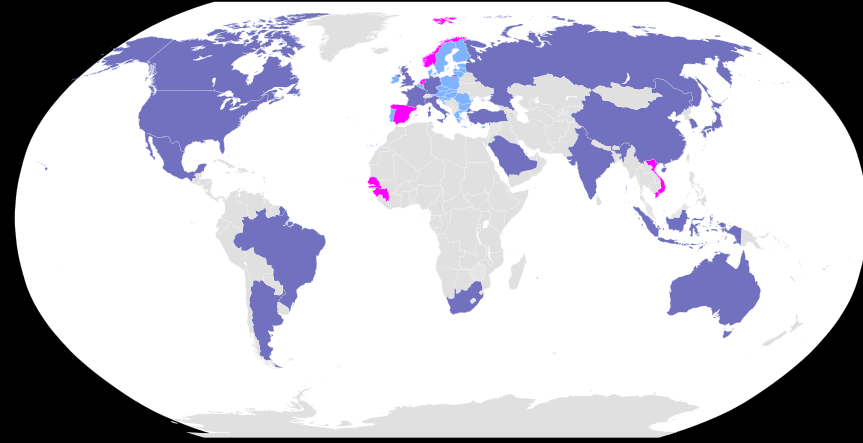
\includegraphics[width=1\textwidth]{G20.png}
\end{figure}
\end{frame}
%--------------------------------------------------------------------

\begin{frame}
\frametitle{G20 Seoul Summit Declaration, 2010}
“We are committed to take action at the national and international level to raise standards, and ensure that our national authorities implement global standards developed to date, consistently, in a way that ensures a level playing field, a race to the top and avoids fragmentation of markets, protectionism and regulatory arbitrage. In particular, we will implement fully the new bank capital and liquidity standards and address too-big-to-fail problems.”\\
\tiny{Source: The Seoul summit document. http://online.wsj.com/public/resources/documents/G20COMMUN1110.pdf}


\end{frame}
\begin{frame}
\frametitle{Basel Committee on Banking Supervision}
\begin{figure}
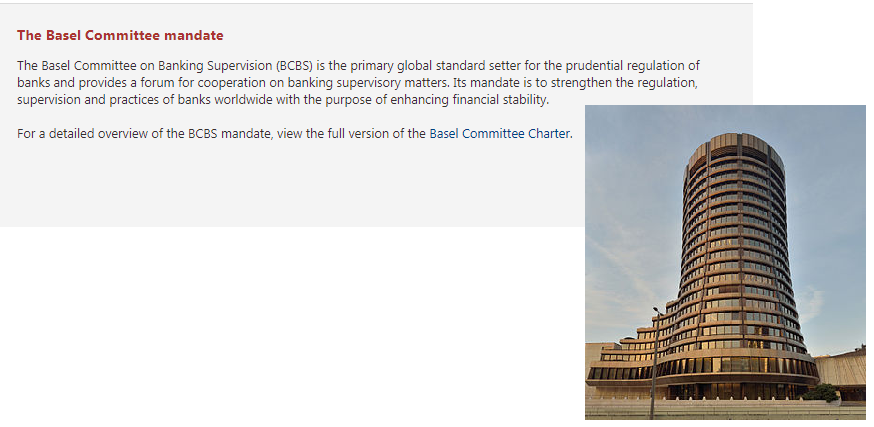
\includegraphics[width=1 \textwidth]{BCBS1.png}
\end{figure}
\tiny{Source https://www.bis.org/bcbs/about.htm}
\end{frame}



\begin{frame}
\frametitle{Basel Committee on Banking Supervision}
In response to the 2007-2009 global financial crisis, the BCBS issued what is referred to as Basel II.5 as an amendment to Basel II
\begin{itemize}
\item Basel II.5 designed to better capture credit risk in the “trading book” of a bank
\item Trading book $\rightarrow$ to securities that a bank would not hold to maturity and would also be accounted for at current market value.
\item intended to prevent strategic but inappropriate placement of
securities in the book that would provide the most favorable accounting treatment at a particular point in time, potentially resulting in a bank having an insufficient capital buffer to mitigate
lending risks
\end{itemize}
\tiny{Source: https://fas.org/sgp/crs/misc/R42744.pdf}
\end{frame}
%-----------------------------------------------------------
\begin{frame}
\frametitle{International Monetary Fund}
Created in 1945, the IMF is governed by and accountable to the 189 countries that make up its near-global membership.
\\
\begin{figure}
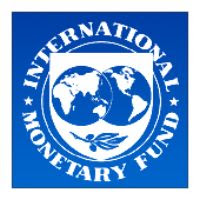
\includegraphics[]{IMF.png}
\end{figure}
The IMF is  working to foster global monetary cooperation, secure financial stability, facilitate international trade, promote high employment and sustainable economic growth, and reduce poverty around the world.
\end{frame}


%--------------------------------------------------------------
\begin{frame}
\frametitle{International Monetary Fund}
IMF’s Response to the Global Economic Crisis
\begin{itemize}
\item Creating a crisis firewall
\item Stepping up crisis lending.
\item Helping the world’s poorest.
\item Sharpening IMF analysis and policy advice.
\item Reforming the IMF’s governance.

\end{itemize}


\end{frame}

%=================================================================
\begin{frame}
\begin{center}
 Day 3 Session 4 \\
Global financial crisis - Central bank responses
\end{center}
\end{frame}
\section{The Power of Central Banks and the Future of the Federal Reserve System}\label{Sec::Chapter2}
%
%==================================================================================

% ------------------------------------------------------------------


% ------------------------------------------------------------------

\begin{frame}
	\frametitle{A challenge issued to central banks}
	\begin{itemize}\itemsep10pt
    	\item Central banks operate within legal framework set by regulation
        \item Is it better to prevent bubbles or to mop up after the crash?\\
	        ~\hfill $\Rightarrow$ Pre-crisis: mopping up after the crash
        \item The zero lower bound (why? Cash as alternative)
        \item Monetary policy implementation needs working financial system, in particular working interbank market
        \item \textit{``Unconventional''} monetary policy is set of tools to circumvent zero lower bound
        ~\\
    \end{itemize}
    \textit{``The problem with QE is that it works in practice, but it doesn’t work in theory.''}\\
    ~\hfill Ben Bernanke, Chairman of the Board, Federal Reserve
\end{frame}

% ------------------------------------------------------------------

\begin{frame}
	\frametitle{What is unconventional monetary policy?}
	\begin{minipage}{0.33\textwidth}
    	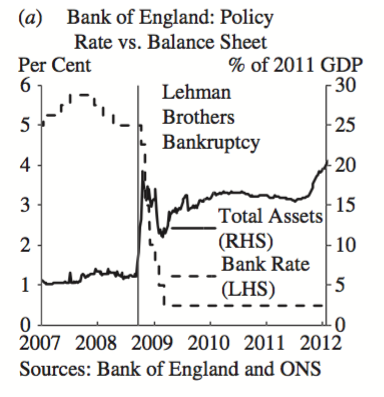
\includegraphics[width=\textwidth]{Figures/BoE_UnconvMonPol.png}
    \end{minipage}\begin{minipage}{0.33\textwidth}
    	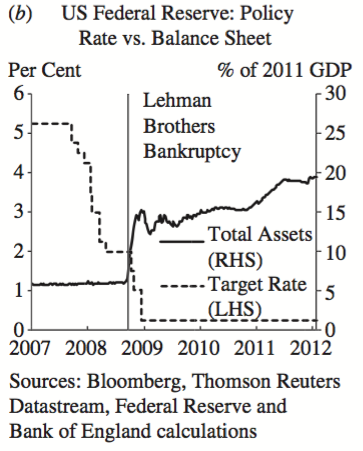
\includegraphics[width=\textwidth]{Figures/Fed_UnconvMonPol.png}
    \end{minipage}\begin{minipage}{0.33\textwidth}
    	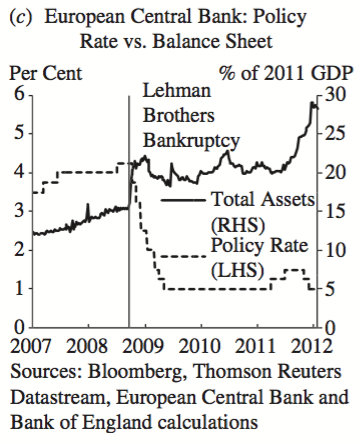
\includegraphics[width=\textwidth]{Figures/ECB_UnconvMonPol.png}
    \end{minipage}
\end{frame}

% ------------------------------------------------------------------

\begin{frame}
\begin{figure}
\frametitle{Quantitative Easing - the basic idea}
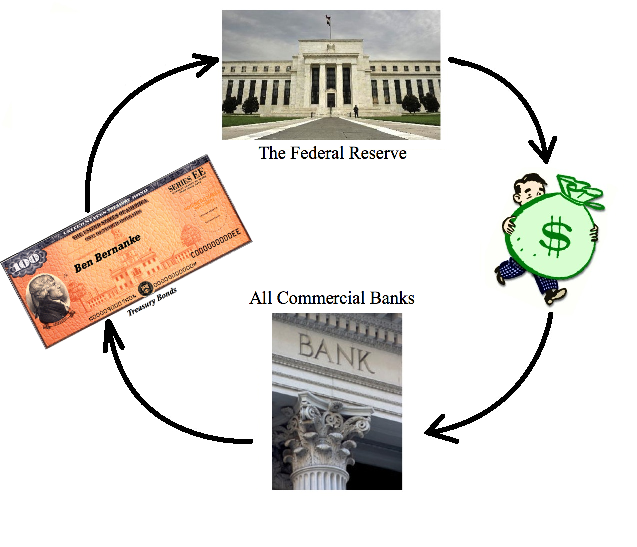
\includegraphics[width=0.8\textwidth]{QE123.png}
\end{figure}
\tiny{Source:http://www.blwinvestments.com/blog/quantitative-easing-20-what-it-means-investor}
\end{frame}
%--------------------------------------
\begin{frame}
	\frametitle{How does QE work in theory?}
   	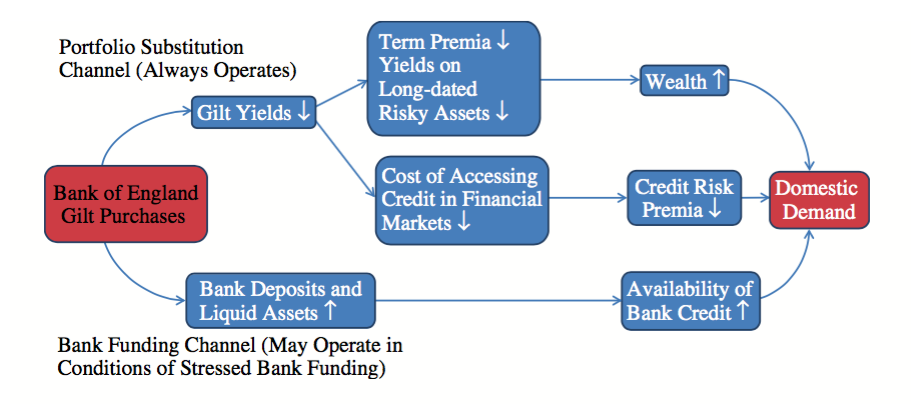
\includegraphics[width=\textwidth]{Figures/How_QE_works.png}
\end{frame}




% ------------------------------------------------------------------

\begin{frame}
	\frametitle{How did QE affect the financial system?}
    \begin{center}
	   	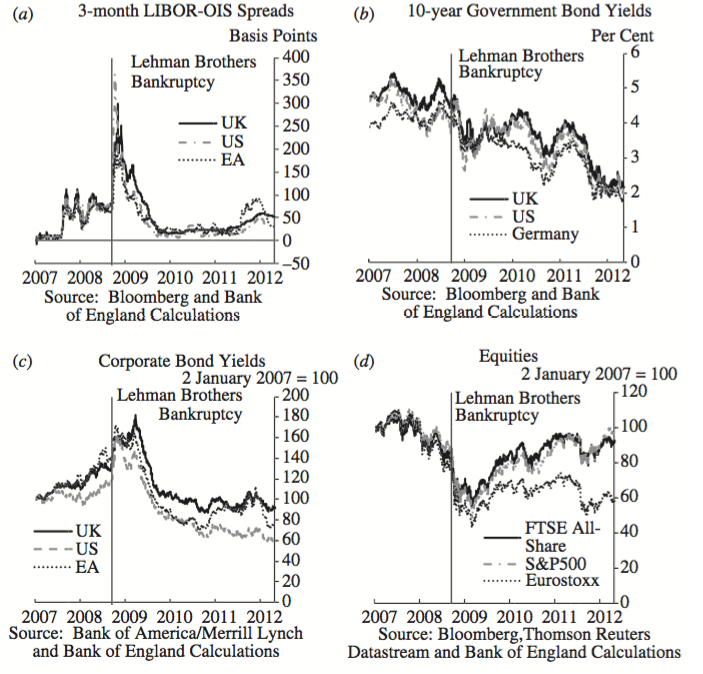
\includegraphics[width=0.8\textwidth]{Figures/FinancialConditions.png}
    \end{center}
\end{frame}

% ------------------------------------------------------------------

\begin{frame}
	\frametitle{How did QE affect the real economy?}
    \begin{center}
	   	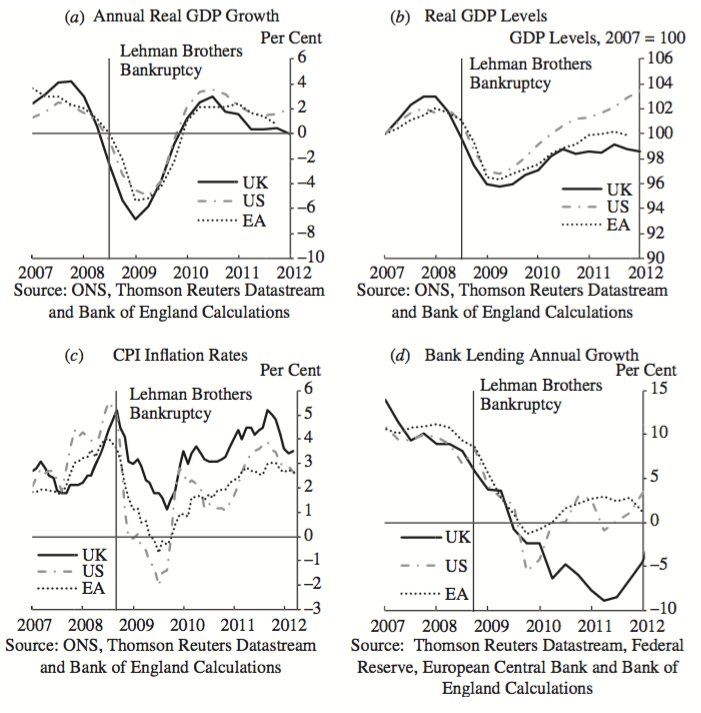
\includegraphics[width=0.8\textwidth]{Figures/MacroIndicators.png}
    \end{center}
\end{frame}

% ------------------------------------------------------------------

\begin{frame}
\frametitle{Central banks and the future of the federal reserve system}
\begin{itemize}\itemsep10pt
\item The Federal Reserve is a large private corporation (SARB is also privately owned)\\
$\Rightarrow$ limits the short run political influences on an economy
\item Dodd-Frank leaves the Fed independent
\begin{itemize}\itemsep5pt
	\item Key influence in monetary policy
	\item Supervision and regulation of individual financial institutions
	\item Supervision and regulation of the financial sector
	\item Its limitation is that it has to answer to congress
\end{itemize}
\end{itemize}
\end{frame}

% ------------------------------------------------------------------

\begin{frame}
\frametitle{Central banks and the future of the federal reserve system}
\begin{itemize}\itemsep10pt
\item The central bank has full control over monetary policy
\item It achieves lower and less volatile inflation rates at no long run cost to output
\item Under the supervision and regulation of the financial sector, it acts as a lender of last resort
\item Used to identify risks to financial stability in the US
\end{itemize}
\end{frame}








%--------------------------------------------------------------------
\begin{frame}
\begin{center}
 Day 3 Session 5 \\
Central banks response 2: Financial stability and systemic risk
\end{center}
\end{frame}

%-----------------------------------------------------------------

\begin{frame}
\frametitle{Policy following the global financial crisis}
as the crisis worsened, almost every country in the world became affected through second round effects, via a decline in consumer confidence which negatively impacted world trade. \\
The main debate globally was the role of monetary policy and the fact that whilst flexible inflation targeting was the most appropriate way to achieve monetary policy objectives in the past, this was no longer the case. \\
There was wide consensus that central banks should adopt a set of multiple objectives:
\begin{itemize}
\item maintain price stability
\item support long-term economic growth and stable employment while still preserving the medium term price stability objective
\item promote financial stability in the financial system
\end{itemize}
\end{frame}

\begin{frame}
\begin{center}
The most recent crisis showed that price stability was not a pre-condition for financial stability (IMF,2013a).
\end{center}
\tiny{Source: Crisis Offers Preliminary Lessons on Fiscal
Policy. IMF Survey online, September 2013.}
\end{frame}



% \begin{frame}
% \frametitle{Central banks (now also) responsible for financial stability}
% This section reviews the state, at 2009, the evolving debates in selected countries and regions namely the United States, the United Kingdom, Germany and the Euro area.\\
% \tiny{Source: https://www.imf.org/external/pubs/ft/wp/2009/wp0970.pdf}
% \end{frame}


%----------------------------------------------------------------


\begin{frame}
\frametitle{US - Financial stability in 2009}
\begin{itemize}
\item  Treasury issued a “Blueprint for a modernized financial regulatory structure” in March 2008
\item Blueprint motivated reform, points out that much of the existing regulatory structure was created more than 70 years ago, and that this structure now “grapples to keep pace with market evolutions” and “faces increasing difficulties in preventing and anticipating financial crises”
\item For example, the US regulation of deposit-taking institutions is characterized by an ineffectual web of agencies, with five federal agencies needing to coordinate between each other in the regulation and resolution of national banks, as well as with state authorities
\item Under the Blueprint proposals, the Fed is to become the overall “market stability regulator.”
\item $\rightarrow$This gives the Fed a formal responsibility for overall financial stability as well as “broad powers” focusing on the overall financial system.

\end{itemize}
\end{frame}

\begin{frame}
\frametitle{US and financial stability}
\begin{itemize}
\item powers of the Fed include
\begin{itemize}
\item authority to collect information from individual institutions
\item to collaborate with other institutions in rulemaking
\item to take corrective action when this is required to preserve overall financial stability
\end{itemize}
\item Blueprint also envisages for the Fed to have a more formal role in the oversight of payment systems, enabling it to “designate” such systems that it deemed systemically important, so as to subject them to formal oversight.
\item A separate federal prudential regulator would oversee all
deposit-taking institutions as well as insurance companies, both of which are envisaged to continue to enjoy explicit government guarantees.
\item The conduct of business regulator would oversee market practices across the financial industry, including securities, insurance, and banking.
\end{itemize}
\end{frame}


% ------------------------------------------------------------------

\begin{frame}
\frametitle{UK and financial stability in 2009}
\begin{itemize}
\item  in response to the experience in dealing with Northern Rock, the authorities issued a consultation paper in July 2008 to strengthen the U.K. framework for financial stability.
\item envisaged a strengthening of the role of the BOE in financial stability, giving it a formal statutory responsibility for financial stability and a leading role in the implementation of a special resolution regime for banks
\item Banking Act 2009 formalizes the role of the BOE in the resolution of financial institutions.
\item It also introduces statutory powers for the central bank in its oversight of systemically-important payment and settlement systems.
\item Greater powers on the part of the BOE will be associated with greater independent accountability: oversight of the BOE’s actions in financial stability will be provided by a new Financial Stability Committee (FSC) as a committee of Court (the nonexecutive supervisory board of the BOE).
\item In addition, steps are being taken to improve the bank’s access to supervisory information.
\end{itemize}
\end{frame}

%------------------------------------------------------------
\begin{frame}
\frametitle{Germany and Financial Stability in 2009}

\begin{itemize}
\item Subprime-related losses (e.g., at Landesbanken, such as Sachsen LB and WestLB, as well as at IKB and Hypo Real), have led to debate on the supervisory framework and the effectiveness of the existing bank resolution framework.
\item Bundesbank and BaFin have long shared a joint responsibility for banking supervision, but there had been a perception that the division of labor had lacked clarity and transparency, leading to potential duplication of effort, undue bureaucratic delay, and the danger that problems might fall through the cracks.
\item new MOU issued in Feb 2008 is meant to clarify the responsibilities of the two agencies and to improve inter-agency cooperation

\end{itemize}

\end{frame}


%----------------------------------------------------------------
\begin{frame}
\frametitle{Euro area and Financial Stability in 2008}
\begin{itemize}
\item In Euro area as a whole, a report from a high-level group issued recommendations intended to overhaul the European structure of financial regulation and supervision.
\item While day-to-day supervision would remain with national authorities, the recommendations contain three new elements:
\begin{enumerate}
\item a macroprudential authority (ESRC), chaired by the ECB and composed of members of the ESCB General Council—that is all EU member countries’ central banks—in addition to the European Commission and the chair of CEBS (Committee for European Banking Supervision)
\item a microprudential authority (ESFS) comprising banking, insurance, and securities committees (CEBS, CEIOPS, and CESR); and
\item a strengthening of the sectoral committees (CEBS, CEIOPS, and CESR) that promotes them to “authorities,” endowed with specific powers, to ensure the consistency of supervision across Europe.
\end{enumerate}
\end{itemize}


\end{frame}



\begin{frame}
\begin{center}
\centering{\Large Day 3 session 6 \\US regulatory response: "Legislation US 2" }
\end{center}
\end{frame}

% ------------------------------------------------------------------

\begin{frame}
\frametitle{Dodd-Frank reform and consumer protection act}
\begin{itemize}
\item The Dodd–Frank Wall Street Reform and Consumer Protection Act was signed into federal law in 2010, passed as a response to the 2007-2008 financial crisis
\item Its goal is to address the increasing propensity of the financial sector to put the entire system at risk and eventually need to be bailed out at taxpayer expense
%\item This bill established a financial stability oversight council (FSOC)
%\item Structure: it has a data center and a research and analysis center
%\item Role is to identify risks to financial stability in the US
\end{itemize}
\end{frame}

% --------------------------------------------------------------------
\begin{frame}
\frametitle{Dodd-Frank reform and consumer protection act}
Major components of the act include:
\begin{itemize}
\item Identifying and regulating systemic risk
\begin{itemize}
\item Sets up a Systemic Risk Council that can deem non-bank financial firms as systemically important, regulate them, and, as a last resort, break them up
\item Establishes the Financial Stability Oversight Council, under the US Treasury responsible for collecting, analyzing, and disseminating relevant information for anticipating future crises
\end{itemize}
\item Expanding the responsibility and authority of the Federal Reserve by granting it authority over all systemic institutions and responsibility for preserving financial stability.
%
\end{itemize}
\end{frame}

% --------------------------------------------------------------------

\begin{frame}
\frametitle{Dodd-Frank reform and consumer protection act}
\begin{itemize}
\item Proposing an end to too-big-to-fail by requiring funeral plans and orderly liquidation procedures for unwinding of systemically important institutions, ruling out taxpayer funding instead requiring that costs be borne by shareholders and creditors, and if required, ex post levies be imposed on other (surviving) large financial firms
\item Reinstating a limited form of Glass-Steagall by limiting bank holding companies to minimal investments in proprietary trading activities, and prohibits them from bailing out these investments.
\end{itemize}
\end{frame}

% --------------------------------------------------------------------
\begin{frame}
\frametitle{Prudential standards}
\begin{itemize}
	\item The act calls for stricter prudential standards for SIFIs based on:
  	\begin{enumerate}\itemsep5pt
      \item Extent of leverage of the firm
      \item Nature of off-balance-sheet exposure
      \item Nature of transactions of the company
      \item Relationship with other significant non-bank financial companies
      \item Source of credit
      \item Extent to which assets are managed
      \item Nature, scope, size , scale, concentration and connectedness
      \item Degree to which it is already regulated
      \item Amount and nature of financial assets
      \item Amount and type of liabilities
	\end{enumerate}
\end{itemize}
\end{frame}

% ------------------------------------------------------------------

\begin{frame}
\frametitle{Policies used to regulate financial companies}
\begin{itemize}\itemsep10pt
\item One of the main drivers of a firm's contribution to systemic risk is the co-movement of its assets with those of the aggregate financial sector during a crisis
\item Policies used to regulate financial companies:
\begin{enumerate}\itemsep5pt
\item Risk-based capital requirements
\item Leverage limits
\item Liquidity requirements
\item Resolution plan and credit exposure report requirements
\item Concentration limits
\item A contingent capital requirement
\item Enhanced public disclosures
\item Short-term debt limits
\item Overall risk management requirements
\end{enumerate}
\end{itemize}
\end{frame}

% ------------------------------------------------------------------

\begin{frame}
\frametitle{Evaluation of the Dodd-Frank Act (from SR perspective)}
The classification based criteria for determining systemic institutions can be supplemented with market based measures of systemic risk:
\begin{itemize}\itemsep10pt
  \item Stock market data can be used to identify firms with greater exposure to losses in a crisis
  \item This helps to prevent regulatory arbitrage
  \item Method one: Marginal expected shortfall (MES)
  \item Estimates the loss of equity a firm can expect during a crisis
  \item A high MES indicates greater risk of bankruptcy or regulatory intervention
\end{itemize}
\end{frame}

% ------------------------------------------------------------------

\begin{frame}
\frametitle{Evaluation of the Dodd-Frank Act (from SR perspective)}
Market based measures of systemic risk:
\begin{itemize}\itemsep10pt
	\item Method two: Look at the interconnectedness of firms
    \item Understanding interconnectedness is key to measuring systemic risk, as its precise nature may be entirely different in a stressed scenario
 	\item This can be achieved through the creation of a report detailing the exposure of firms to other institutions through derivative contracts and interbank liabilities
  	\item This requires legislation that compels reporting
  	\item Criteria when looking at each important institution:
	\begin{enumerate}\itemsep5pt
		\item Look at dominant risk factors
		\item Look at counterparties in terms of potential exposure to stress
	\end{enumerate}
    Challenge: financial interconnectedness
\end{itemize}
\end{frame}

% ------------------------------------------------------------------
\begin{frame}
\frametitle{Stress tests}
\begin{itemize}\itemsep10pt
\item A stress test is a probabilistic scenario analysis to determine the needed capital buffer in a crisis
\item The Dodd-Frank Act calls for systemic institutions to be subject to periodic stress tests
\item Stress tests require a fully transparent approach
\item Benefit of transparency:
\begin{enumerate}
\item Releases valuable capitalization information
\item Counter-party exposure information will also be available
\end{enumerate}
\item This testing helps to address operational risk
\item Operational risk is typically attributed to deficiencies in corporate processes, its people and technology
\end{itemize}
\end{frame}
% \begin{frame}
% \begin{center}
% Case study day 3 = Ireland
% Paper day 3 = to be decided
% \end{center}
% \end{frame}

% ------------------------------------------------------------------
% ------------------------------------------------------------------
\begin{frame}
\begin{center}
\centering{\Large Two Forms of Systemic Risk}
\end{center}
\end{frame}
% ------------------------------------------------------------------
% ------------------------------------------------------------------

\begin{frame}
 \begin{itemize}
  \item Example of \mcdr{contagion} vs. common shocks through a \mcdr{fire-sale mechanism}.
 \end{itemize}
\color{black}
\begin{table}
 \begin{tabular}{|c|c||c|c|}
  \hline
  Assets & & Liabilities & \\
  \hline
  Loans to Customers & 100 & Retail Deposits & 130\\
  Loans to B & 30 & Borrowing from B & 30\\
  Loans to C & 30 & Borrowing from C & 30\\
  Other securities & 40 & Equity Capital & 10\\
  Total & 200 & & 200\\
  \hline
 \end{tabular}
\caption{Balance sheet of bank A}
\end{table}

\end{frame}

\begin{frame}
\vspace{5mm}
\color{black}
\begin{table}
 \begin{tabular}{|c|c||c|c|}
  \hline
  Assets & & Liabilities & \\
  \hline
  Loans to Customers & 100 & Retail Deposits & 130\\
  Loans to A & 30 & Borrowing from A & 30\\
  Loans to C & 30 & Borrowing from C & 30\\
  Other securities & 40 & Equity Capital & 10\\
  Total & 200 & & 200\\
  \hline
 \end{tabular}
\caption{Balance sheet of bank B}
\end{table}
\vspace{-5mm}
\begin{table}
 \begin{tabular}{|c|c||c|c|}
  \hline
  Assets & & Liabilities & \\
  \hline
  Loans to Customers & 100 & Retail Deposits & 130\\
  Loans to A & 30 & Borrowing from A & 30\\
  Loans to B & 30 & Borrowing from B & 30\\
  Other securities & 40 & Equity Capital & 10\\
  Total & 200 & & 200\\
  \hline
 \end{tabular}
\caption{Balance sheet of bank C}
\end{table}
\end{frame}

\begin{frame}
 \begin{itemize}
  \item The banks are \mcdbl{completely symmetric} w.r.t. deposits, borrowings, securities and equity.
 \end{itemize}
% \pause
\begin{block}{The domino case}
  \begin{itemize}
  \item Suppose that A makes a \mcdr{loss} of 40 on it's loans.
% \pause
  \item This \mcdr{wipes out} it's equity.
% \pause
  \item It has a \mcdr{shortfall} of 30 on it's liabilities.
% \pause
  \item This shortfall is divided up amongst B and C, each suffering a shortfall of 15 on their \mcdr{interbank lendings}.\\
        \hfill \mcdr{$\Rightarrow$ B and C are wiped out as well!}
 \end{itemize}
\end{block}

\end{frame}

\begin{frame}
\begin{block}{Beyond the domino model...}
  \begin{itemize}
   \item Bank A makes \mcdr{losses} of 5 on it's loan book, halfing it's \mcdbl{equity capital} to 5.
% \pause
   \item The \mcdbl{leverage ratio} (ratio of assets to equity capital) of A increases from 20 (200/10) to 39 (195/5), putting the bank close to, or
 below the \mcdgr{capital adequacy ratio}.
% \pause
   \item This forces A to sell some of it's securities.
% \pause
   \item They were originally worth 40, but since A has to get rid of them in a \mcdr{fire-sale}, the bank sells half of them and recoups only 18.
% \pause
   \item This reduces the bank's equity capital to 1.
% \pause
  \end{itemize}
\end{block}

\end{frame}

\begin{frame}
\begin{block}{Beyond the domino model (ctd.)...}
  \begin{itemize}
   \item B and C are now hit with \mcdr{two problems}:
   \begin{enumerate}
    \item Since A has been selling it's securities in a fire-sale, the securities of B and C are now worth only 36. This \mcdr{reduces their equity capital} to 6.
% \pause
    \item Needing to shrink their balance sheets and worried about A's solvency, they decide \mcdr{not to roll-over their loans} to A.
   \end{enumerate}
% \pause
   \item A now has to repay the loans to B and C, but with \mcdr{almost no equity} and the \mcdr{value of it's securities falling}, it fails to do so.
% \pause
   \item B and C now realize losses on their loans to A and also on their securities.\\
\hfill\mcdr{$\Rightarrow$ B and C are just as vulnerable as A}
  \end{itemize}
\end{block}
\end{frame}

% ==================================================================
%
\section{Alternatives to Regulation}
%
% ==================================================================
\begin{frame}
\begin{center}
\centering{\Large Taxing Systemic Risk}
\end{center}
\end{frame}

% ------------------------------------------------------------------

\begin{frame}
\frametitle{Systemic risk and the financial crisis}
\begin{itemize}
\item The stock market declined by $42$\% in the US during the crisis
\item Global GDP declined by $0.8$\%
\item Some financial institutions contributed more to the failure than others
\item This contribution of the capital shortfall represents a negative externality
\item A way to remove this would be the introduction of a tax on the systemic risk of financial firms
\end{itemize}
\end{frame}

% ------------------------------------------------------------------

\begin{frame}
\begin{itemize}\itemsep10pt
\item This is opposite to what Dodd-Frank Act does
\item Rather than taxation, they focus on governments ability to contain systemic risk through the design of capital adequacy requirements
\item Systemic risk taxation needs to be equally imposed across the financial sector
\item Interconnectedness of financial sector means every financial firm gets affected by one firms decline in equity
\item Financial firms:
\begin{enumerate}\itemsep5pt
\item Commercial banks
\item Investment banks
\item Money market funds
\item Insurance firms
\item Hedge funds
\item Private equity firms
\end{enumerate}
\end{itemize}
\end{frame}

% ------------------------------------------------------------------

\begin{frame}
\frametitle{Three challenges to regulating systemic risk}
\begin{itemize}\itemsep10pt
\item Identify and measure systemic risk
\item Develop an optimal policy to have firms internalize systemic risk costs
\item Ensure that the policy can be implemented
\end{itemize}
\end{frame}

% ------------------------------------------------------------------

\begin{frame}
\frametitle{Model}
\begin{itemize}\itemsep10pt
\item Banking system where each bank has limited liability and maximizes shareholder value
\item Regulators provide a safety net for financial firms
\item Systemic risk emerges when the banking sector's equity capitalization is lower than a fraction of its total assets
\item Costs of systemic risks are proportional to the size of this shortfall
\item This implies that taxing individual banks is optimal
\end{itemize}
\end{frame}

% ------------------------------------------------------------------

\begin{frame}
\frametitle{Systemic risk tax}
\begin{itemize}\itemsep10pt
\item Systemic risk tax is calculated by:
\begin{enumerate}\itemsep5pt
\item Expected loss of firm upon default: Financial firms must pay for guarantees they receive
\item Expected systemic costs in a crisis multiplied by firm contribution to costs: The risk needs to be priced and the financial firms need to internalize the costs of a negative externality
\end{enumerate}
\end{itemize}
\end{frame}

% ------------------------------------------------------------------

\begin{frame}
\frametitle{Difficulties implementing policy}
Measuring systemic risk:
\begin{itemize}\itemsep10pt
\item It is the fraction of expected losses made by financial firms in a systemic event
\item Expected systemic cost: Measures the level of systemic risk
\item It is the \% contribution of the institute to costs occurred in a financial sector collapse
\end{itemize}
\end{frame}

% ------------------------------------------------------------------

\begin{frame}
\frametitle{Implementing tax on systemic risk}
\begin{itemize}\itemsep10pt
\item There are two schemes to charge for systemic risk:
\begin{enumerate}\itemsep5pt
\item Market-based discovery of the price of systemic risk insurance
\item Direct regulatory tax
\end{enumerate}
\item Empirically, it is based on time series data as to what causes a crisis
\item Mainly, by calculating the probability of a crisis occurring
\item The following is taken into account when calculating the probability of a crisis:
\begin{enumerate}\itemsep5pt
\item System-wide leverage
\item Asset bubbles
\item Market volatility
\end{enumerate}

\end{itemize}
\end{frame}

% ------------------------------------------------------------------

\begin{frame}
\begin{itemize}\itemsep10pt
\item By measuring the costs of past crises and the probability of a crisis results in finding expected costs
\item The advantage is that regulators can adjust expected costs, making them countercyclical
\item It can then be used to determine which institutions contribute to risk
\item As well as the firms contribution to sector-wide equity losses when the sector fails
\item It can be observed in the table as follows
\end{itemize}
\end{frame}

% ------------------------------------------------------------------

\begin{frame}
\begin{figure}
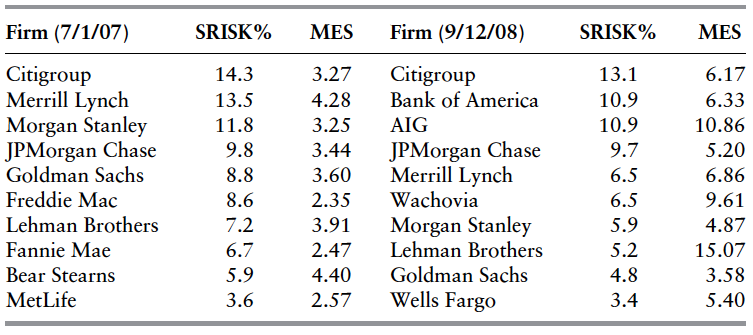
\includegraphics[width=\textwidth]{table5_1.png}
\caption{Risk measures for the most systemic financial firms}
\end{figure}
\end{frame}

% ------------------------------------------------------------------

\begin{frame}
\begin{itemize}\itemsep10pt
\item Provides risk measures from the top 100 systemic financial firms
\item During July 2007 and September 2008, firms not only fail but also create most of the systemic risk
\item It can be seen that most of the systemic risk is captured by a few firms
\item The increase in the MES measure indicates the start of a crisis
\item Regulators estimate the \% contribution of each financial firm to aggregate capital shortfall of the financial sector
\item If implemented correctly, financial firms would optimally choose to be less levered and hold less systemic risky assets
\end{itemize}
\end{frame}

% ------------------------------------------------------------------

\begin{frame}
\frametitle{Moral hazard}
\begin{itemize}\itemsep10pt
\item Moral hazard is mitigated under taxation because government prices and charges for both firm risk and systemic risk
\item However, firm behavior is unobservable hence premiums on systemic risk is set
\item As well as capital requirements and restrictions are imposed
\item This results in firms imposing its own behavior
\item It imposes a penalty function in bad states to avoid excessive risk taking by firms
\item The problem with this is that a system of limited liability imposed is irrelevant as shareholders are mitigated
\end{itemize}
\end{frame}

% ------------------------------------------------------------------

\begin{frame}
\frametitle{Dodd-Frank Act}
\begin{itemize}\itemsep10pt
\item This act addresses systemic risk differently to direct tax regulation
\item It prefers to manage systemic risk
\item Disadvantage of using this approach is that it won't reduce systemic risk sufficiently as it may shift to another part in the system
\item Effectiveness of the act and how it analyzes it:
\begin{enumerate}\itemsep5pt
\item Identify and measure systemic risk
\item Uses systemic risk to create an optimal policy
\item Ensure that the policy has no future regulatory arbitrage and eliminates moral hazard
\end{enumerate}
\end{itemize}
\end{frame}

% ------------------------------------------------------------------

\begin{frame}
\frametitle{Measuring of systemic risk}
A firm is systemic if:
\begin{itemize}
\item Material financial distress at company level can pose a threat to financial stability
\item Nature, scope, size, scale, concentration, interconnectedness or a mix of company's activities affect financial stability as a whole
\item In particular, regulators look at:
\begin{enumerate}
\item Amount and nature of company's financial assets
\item Amount and nature of company's financial liabilities
\item Extent of company's leverage
\item Extent and nature of off-balance sheet exposures
\item Transactions and relationship with other financial firms
\item As as source of credit for households, businesses, state and local government
\item Degree at which a company is regulated
\end{enumerate}
\item However, omitting the co-movement of a firms asset returns with aggregate financial sector during a crisis
\end{itemize}
\end{frame}

% ------------------------------------------------------------------

\begin{frame}
\frametitle{Reducing systemic risk}
Reducing systemic risk is done by implementing stricter standards such as:
\begin{itemize}
\item Risk-based capital requirements
\item Leverage limits
\item Liquidity requirements
\item Contingent capital requirements
\item Resolution plan and credit exposure reports
\item Enhanced public disclosures
\item Concentration limits
\item Short-term debt limits
\item Risk management requirements
\end{itemize}
\end{frame}

% ------------------------------------------------------------------

\begin{frame}
\frametitle{Mitigating moral hazard}
\begin{itemize}
\item The Dodd-Frank Act fails when it comes to moral hazard due to the free rider problem
\item Free-rider problem: Firms that have large amounts of systemic liabilities aren't allowed to fail by regulators
\end{itemize}
\end{frame}

% ------------------------------------------------------------------

\begin{frame}
\frametitle{Tax on systemic risk}
Public-private insurance plan is required:
\begin{itemize}\itemsep10pt
\item Regulated firms would have target capital of current assets
\item Allows regulators to determine the proportionate share of expected losses contributed in a crisis
\item Fees paid to insurance company's are negated from the firms total systemic tax
\item Firms continuously pay tax and acquire insurance
\item Future expected bailouts need to be priced separately
\end{itemize}
\end{frame}



\begin{frame}
\frametitle{Basel III and the Dodd-Frank Act}
Improvements in the Dodd-Frank Act are possible as follows:
\begin{itemize}
\item Closing major capital loopholes
\item Relying less on ratings agencies
\end{itemize}
~\\
Dodd-Frank Act improvements:
\begin{itemize}
\item Addresses conflict of interest between rating agency business model and governments regulatory reliance on ratings
\item Includes off-balance-sheet activities in computing capital requirements
\item With respect to derivatives:
\begin{enumerate}
\item Margin requirements
\item Reporting to data repositories
\item Providing authority for prudential regulators
\end{enumerate}
\end{itemize}
\end{frame}

\begin{frame}
\begin{itemize}\itemsep10pt
\item It still doesn't take into account the effect of shifting financial activities elsewhere will have on the financial sector
\item Purpose of Basel Accord: common risk-based assessment of bank assets and required capital levels
\item Basel III:
\begin{enumerate}\itemsep5pt
\item Stricter on what constitutes as capital
\item Minimum leverage ratio
\item Creates liquidity ratio that banks are required to abide by
\end{enumerate}
\item Basel III doesn't take into account shadow banking nor regulatory arbitrage
\end{itemize}
\end{frame}

\begin{frame}
\frametitle{Capital requirements}
\begin{itemize}\itemsep10pt
\item Dodd-Frank Act and Basel III provide explicit maximum leverage ratio and minimum capital ratio's
\item Risk-based capital and leverage capital ratio's will be applied to bank holding companies and systemically important institutions
\item The current Basel II total capital ratio of 8\% is expected to increase under Basel III as in the following table
\end{itemize}
\end{frame}

\begin{frame}
\begin{figure}
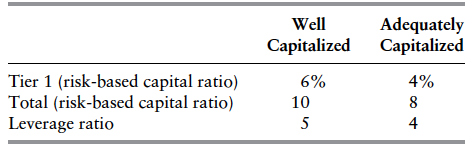
\includegraphics[width=\textwidth]{6_1.png}
\caption{Capital adequacy standards}
\end{figure}
\end{frame}

\begin{frame}
\begin{itemize}\itemsep10pt
\item These requirements are to be enacted within 18 months, exempting small institutions
\item The definition of capital in Dodd-Frank Act and Basel III don't perfectly coincide, Leverage ratio in Basel III is lower, i.e. 3\%
\item Dodd-Frank Act goes further for SIFIs to "maintain a debt-to-equity ratio" of no more than 15 to 1 (leverage ratio of 6.5\%)
\end{itemize}
\end{frame}

\begin{frame}
\begin{itemize}\itemsep10pt
\item The act requires additional capital requirements as follows:
\begin{enumerate}
\item Significant volumes of activity in derivatives, securitized products purchased and sold
\item Volumes of activity in financial guarantees purchased and sold, securities borrowing, repurchase agreements and reverse repurchase agreements
\end{enumerate}
\item Concentrations in market share for any activity that disrupts financial markets
\item Common in the Dodd-Frank Act and Basel III: Establishes capital regulations that have to be countercyclical
\item This allows for the amount of capital required to be maintained by a company, increases in times of economic contraction, consistent with safety and soundness of a company
\end{itemize}
\end{frame}

\begin{frame}
\frametitle{Limitations}
\begin{itemize}\itemsep10pt
\item Belief that higher capital requirements are costly
\item Capital is defined as equity capital
\item The value of a firm's assets will be independent of how those assets were financed
%\item Given that systemic costs to leverage is higher, it leads to higher capital requirements which is socially costly
\item How to accurately measure leverage at institution level
\item Depends on whether one believes the agency problems of LCFI's are due to conflict of interest
\item Banks dislike capital requirements
\end{itemize}
\end{frame}

\begin{frame}
\begin{itemize}\itemsep10pt
\item Dodd-Frank Act and Basel III don't look at why equity financing is more costly than debt financing
\item Examples:
\begin{enumerate}\itemsep5pt
\item Number of firms used an accounting loophole to temporarily reduce reported leverage
\item Lehman Brother's repo 150 activities reduced reported leverage by 50 billion dollars
\item April 2010: NY Federal reserve bank showed 18 banks decline their net short-term borrowings in the repo market
\end{enumerate}
\end{itemize}
\end{frame}

\begin{frame}
\frametitle{Liquidity requirements}
\begin{itemize}\itemsep10pt
\item Arises because regulated institutions have fragile structures i.e. holding assets within long-term duration or low liquidity
\item Liabilities are highly liquid in the short term
\item Imposes liquidity requirements to reduce a run
\item Requires a proportion of short-term funding must be liquid assets
\item This decreases the probability of runs because
\item These institutions take on carry trades and holding long-term asset-backed securities
\end{itemize}
\end{frame}

\begin{frame}
Basel III outlines two ratios that financial institutions as:
\begin{itemize}\itemsep10pt
\item Liquidity coverage ratio: bank's high-quality liquid assets as a ratio of their net cash flow over a 30 day period
\item Net stable funding ratio: amount of stable funding over required amount of stable funding
\item Assumes that the probability and size of losses associated with default are similar between the two classes of securities
\end{itemize}
\end{frame}

\begin{frame}
\frametitle{Capital}\itemsep10pt
How to measure the capital of a financial institution:
\begin{itemize}
\item Regulatory capital represents a buffer against a decline in the value of a firm's assets against its obligations
\item Doesn't contain a significant debt feature: commitment for future repayment
\item According to the Dodd-Frank Act allows to conduct a study of the use of hybrid capital instruments as a component of Tier 1 capital for banking institutions
\item Basel III includes a fraction (15\%) of Tier 1 capital to include equity investments, mortgage servicing right and deferred tax assets
\end{itemize}
\end{frame}

\begin{frame}
\frametitle{Example}
\begin{itemize}\itemsep10pt
\item Trust preferred securities (TruPSs) are hybrid securities that have debt and equity securities
\item Holding company issues junior subordinated debt to a trust security (has a 100\% ownership of trust)
\item Guarantees that an interest and principal payment of the TruPSs
\item It doesn't have characteristics that are required for securities included in Tier 1 capital
\item Dodd-Frank Act requires banks to phase out TruPSs
\item It gives banks with more than 100 billion dollars in capital to phase out these securities
\item Upto 10 years for institutions with capital between 15 billion and 100 billion dollars
\item It exempts small banks with capital less than 15 billion dollars
\end{itemize}
\end{frame}

\begin{frame}
\frametitle{Contingent capital}
\begin{itemize}
\item It is a hybrid claim that allows for there to be debt in good times but automatically converts it into an equity claim in bad times (uninsured)
\item Example.1: Lloyd's bank issued capital in November 2009 as part of its capital raising program
\item It ensures banks maintain a sufficient level of capitalization
\end{itemize}
\end{frame}

\begin{frame}
\begin{figure}
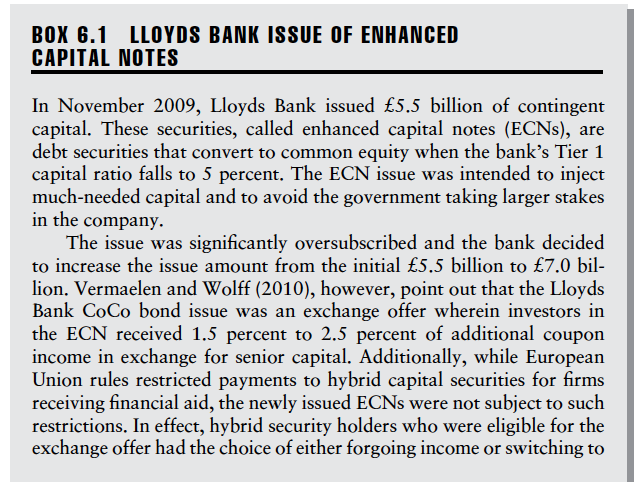
\includegraphics[width=\textwidth]{6_2.png}
\end{figure}
\end{frame}

\begin{frame}
\begin{figure}
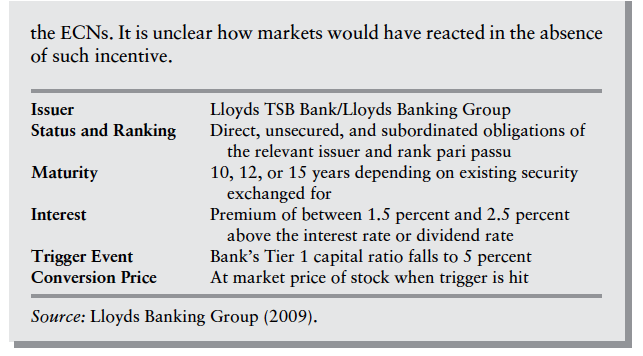
\includegraphics[width=\textwidth]{6_3.png}
\end{figure}
\end{frame}

\begin{frame}
\frametitle{Example.2: Rabobank issued capital on march 2010}
\begin{figure}
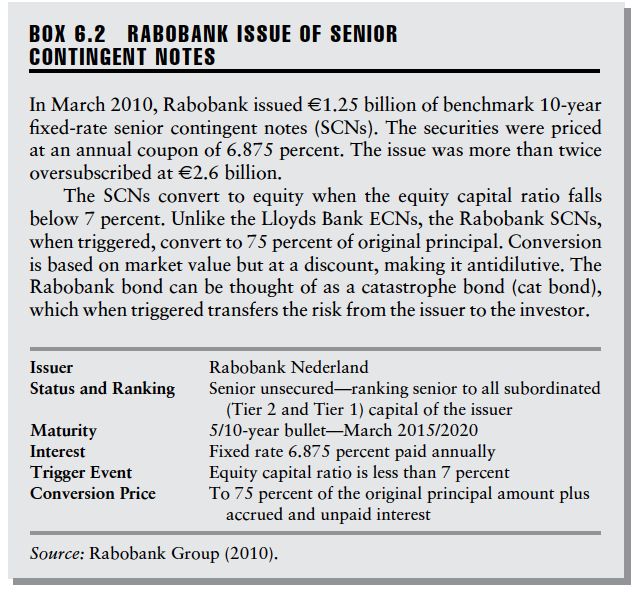
\includegraphics[width=0.8\textwidth]{6_4.png}
\end{figure}
\end{frame}

\begin{frame}
\frametitle{Contingent capital}
\begin{itemize}
\item Ability to limit ex ante risk-taking and buildup of systemic risk
\item Useful to deal with distress when complex contingents charcaterize a firms balance sheet
\item Relative attractiveness to standard capital and liquidity requirements\\
~\\
\item However, not able to come up with international standards of banking regulation
\item As well as it is not adequate for containment of ex post distress in all contingencies
\end{itemize}
\end{frame}

\begin{frame}
\frametitle{Summary of various contingent capital schemes and key features}
\begin{figure}
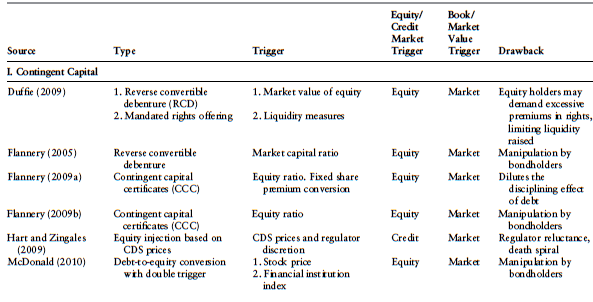
\includegraphics[width=\textwidth]{6_5.png}
\end{figure}
\end{frame}

\begin{frame}
\frametitle{Summary continued}
\begin{figure}
\includegraphics[width=\textwidth]{6_6.png}
\end{figure}
\end{frame}

\begin{frame}
\frametitle{Contingent capital injection}
\begin{itemize}\itemsep10pt
\item Based on reverse convertible debenture
\item It is debt that converts into equity when triggered
\item Schemes differ on the type of trigger
\item Triggers:
\begin{enumerate}\itemsep5pt
\item Rule-based: On books/market value subject to opportunistic manipulation by bondholders
\item Discretionary trigger: based on aggregate market measures
\end{enumerate}
\item leads to a rapid decline in prices i.e. death spiral
\end{itemize}
\end{frame}

\begin{frame}
\frametitle{Contingent capital insurance}
\begin{itemize}
\item Tax based on bank's own contribution to systemic risk
\item Taxes go to a regulator and when a systemic even occurs the regulator determines which firms receive support
\item Liability enhanced equity: an increase in liability is associated with equity
\item Regulators impose higher capital requirements
\end{itemize}
\end{frame}

\begin{frame}
\begin{center}
\centering{\Large Large banks and the Volcker rule}
\end{center}
\end{frame}

\begin{frame}
\frametitle{Overview}
\begin{itemize}
\item Most of the systemic risk in the United States today is from the six largest bank holding companies — Bank of America, JPMorgan Chase, Citigroup, Wells Fargo, Goldman Sachs, and Morgan Stanley
\item These large, complex financial institutions (LCFIs) will still
report to the same regulators as before, whose effectiveness in averting prior crises was sorely lacking
\item LCFIs can be defined as financial intermediaries engaged in some combination of commercial banking, investment banking, asset management, insurance, and/or the payments system, whose failure poses a systemic risk to the financial system as a whole
\item The following table lists the market value and assets of the largest 24 US financial firms in June 2007
\item Shows that US based LCFIs include not just commercial banks but other such financial intermediaries
\end{itemize}
\end{frame}

\begin{frame}
\begin{figure}
\includegraphics[width=0.6\textwidth]{7_1.png}
\caption{Market value and assets of 24 US firms in 2007}
\end{figure}
\end{frame}

\begin{frame}
\frametitle{LCFIs and the financial crisis}
\begin{itemize}
\item The financial crisis caused systemic failure despite central bankers implementing risk-adjusted minimum capital adequacy standards
for banks
\item The crisis spread from the banking sector to the financial world to the real economy, driving it into a steep recession
\item Most of the LCFIs survived because they managed to shift risks by exploiting loopholes in regulatory capital requirements
\item This was financed largely by debt holders who correctly anticipated de facto government guarantees
\item Included insured and uninsured depositors and creditors
\end{itemize}
\end{frame}

\begin{frame}
\frametitle{The economics of LCFIs and its model}
\begin{itemize}
\item The structural form of competition between firms active in a given financial intermediation function or in multiple functions should have a comparative advantage in that area
\item If there are significant economies of scale or economies of scope with respect to either costs or client segments,there are advantages in the size, the range of activities, or the geographic scope or client breadth of those firms that are the most successful
\item The following figure shows the market for financial services as a matrix of clients, products, and geographies
\end{itemize}
\end{frame}

\begin{frame}
\begin{figure}
\includegraphics[width=\textwidth]{7_2.png}
\caption{Market for financial services as a matrix of clients, products, and geographies}
\end{figure}
\end{frame}

\begin{frame}
\begin{itemize}
\item Financial firms want to allocate available resources to those cells in the matrix (market segments) that promise to yield the highest risk-adjusted returns
\item Attribute costs, returns, and risks appropriately to specific cells in the matrix
\item The cells themselves must be linked together in a way that recognizes and maximizes synergies
\item Client-driven linkages (horizontal arrows in the figure) exist when a financial institution can supply financial services more efficiently to either the same or another client in the same group in the same or different geographies
\end{itemize}
\end{frame}

\begin{frame}
\begin{itemize}
\item Risk mitigation results from spreading exposures across clients
\item It includes greater earnings stability to the extent that income streams from different clients or client segments are not perfectly correlated
\item Product-driven linkages (vertical arrows) exist when a firm can supply a financial service in a more competitive manner
\item Again, risk mitigation is to the extent that net revenue streams from different products are not perfectly correlated
\item Geographic linkages (lateral arrows) are important when an institution can service a particular client or supply a particular service more efficiently in one geography
\item To get maximum returns from this strategic positioning matrix,
firms need to know the size, growth and competitive dynamics of
specific market segment
\item As well as, the costs and the risks embedded in their overall portfolio of activities
\end{itemize}
\end{frame}

\begin{frame}
\begin{itemize}
\item The existence of large and complex systemic financial intermediaries suggests one of several possibilities:
\begin{enumerate}
\item The benefits of size and complexity do in fact exceed their costs
\item there are widespread failures in market discipline and effective corporate governance
\item size and complexity result in an unpriced subsidy representing a transfer of wealth from society at large to the shareholders and employees of financial intermediaries
\end{enumerate}
\end{itemize}
\end{frame}

\begin{frame}
\frametitle{History of LCFIs}
\begin{itemize}
\item For seven decades, LCFIs were banned from the U.S. financial system
\item The Glass-Steagall provisions of the Banking Act of 1933 mandated a virtually complete separation of investment banking from deposit taking activities
\item It eliminated involvement by firms with a commercial banking charter in the securities business
\item Critics of the banking model feared that bank involvement in securities underwriting had led to increasing their holdings of long-term financial instruments, exposing them to potentially dangerous market, credit and liquidity risk
\item This triggered the collapse of banks nationwide, which in turn had disastrous consequences for the real economy
\end{itemize}
\end{frame}

\begin{frame}
\begin{itemize}
\item 40\% of all US banks failed during this period, undermining their role as financial intermediaries and put the economy into a crisis
\item The Glass-Steagall Act forced the dissolution of the universal banks
\item US investment banks’ share of financial intermediation grew rapidly as financial flows shifted to financial markets
\item By the 1980s, the US financial system had become heavily market dominated
\item While other financial systems remained dominated by universal
banks
\item Another consequence of Glass-Steagall is the progressive dominance of U.S. investment banks in rapidly evolving global capital markets
\item By the late 1980s, commercial banks had gained the limited right to sell investment and insurance products to retail customers
\item As well as the right to operate separately capitalized, size-constrained wholesale securities subsidiaries
\end{itemize}
\end{frame}

\begin{frame}
\begin{itemize}
\item In 2009, the world’s five largest wholesale banks were responsible for the origination of nearly 60\% of all capital market transactions
\item They accounted for $8.97$ trillion of assets, or approximately 55\% of all assets held in the entire US banking system
\item These LCFIs are regulated by weighing the systemic risk of a particular functional activity undertaken by a financial institution against the benefit of that activity
\end{itemize}
\end{frame}

\begin{frame}
\frametitle{Framework to regulate LCFIs}
Functions of firms that have systemic risk:
\begin{itemize}
\item They act as intermediaries i.e. dealers in security markets, repos, and over-the-counter (OTC) derivatives
\item Conduct commercial banking — deposit taking and lending to individuals and institutions
\item Operate investment banking businesses — underwriting security issues and providing advisory services
\item Offer asset management services — managing assets for institutions and individuals
\item Offer brokerage services to individuals, and prime brokerage for hedge funds and other professional investors
\item Conduct proprietary trading — trading on their own accounts, which include internal hedge funds, private equity partnerships, or asset holdings of unhedged securities
\end{itemize}
\end{frame}

\begin{frame}
\begin{itemize}
\item However, regulators need to identify the relevant cost benefit analysis of combining different financial activities
\item Advantage of LCFIs is that the securities markets have become highly integrated and fluid as a result of securitization, global linkages, derivatives and new forms of market innovation
\item A second argument is that to follow the Glass-Steagall approach
in today’s globalized marketplace, universal banking would have to be prohibited everywhere
\item Overall, LCFIs create greater systemic risk
\end{itemize}
\end{frame}

\begin{frame}
\frametitle{Dodd-Frank Act}
Size constraints:
\begin{itemize}
\item There is the prohibition on the size of financial institutions through mergers if the combined firm’s total liabilities exceed 10\% of aggregate consolidated liabilities of all financial companies in the US
\item Expected intense lobbying activity by firms actually or potentially subject to the 10\% ceiling could have the limit raised, triggering even greater industry consolidation and exposure to systemic risk
\item the US size constraint does reduce the growth prospects of such entities into ever larger firms even though it does not call for breaking up large financial institutions into smaller entities
\item Any institution with more than 10\% of the entire financial
sector’s liabilities is systemic
\item The size cap would therefore help limit the too-big-to-fail problem
\end{itemize}
\end{frame}

\begin{frame}
\begin{itemize}
\item The reverse is not true, as a number of institutions with less than 10\% of liabilities in the system are also systemic
\item After new prudential standards have been implemented, a financial firm represents a systemic threat
\item Activities that constitute the source of that threat could be terminated, carved out or sold to separate unaffiliated financial firms
\item Solutions to this:
\begin{enumerate}
\item Terminating one or more activities
\item Imposing conditions on the manner in which a financial holding company subject to stricter standards conducts one or more activities
\item Limiting the ability to merge with, acquire, consolidate
with, or otherwise become affiliated with another company
\item restricting the ability to offer a financial services or products
\end{enumerate}
\item The disposal of specific LCFI holdings are last-resort measures that have to be approved by a two-thirds vote of the Financial Stability Oversight Council
\item It also allows for bringing non-financial companies posing a systemic threat under the Federal Reserve regulatory umbrella
\end{itemize}
\end{frame}

\begin{frame}
\frametitle{Modified Volcker rule}
\begin{itemize}
\item Any implicit federal guarantee should be limited to a relatively small number of important banking institutions and to core banking functions
\item To include propriety trading: engaging as a principal for the trading account of the banking entity or nonbank financial company supervised by the Board in any transaction
\item LCFIs had already prepared the ground by arguing that proprietary
trading operations were not the cause of the 2007 to 2009 financial crisis
\item The 2009 balance sheets of the four largest banks — JPMorgan Chase, Bank of America, Citigroup, and Wells Fargo — shows holdings of $1.1$ trillion dollars worth of available-for-sale securities
\item An expanded Volcker Rule that extends the definition of proprietary trading to asset-backed security holdings by financial intermediaries
\end{itemize}
\end{frame}

\begin{frame}
\begin{itemize}
\item Other institutions without guarantees such as mutual
funds, pension funds, hedge funds, sovereign wealth funds, and non-systemic insurance companies can step into the breach as banks withdraw from the asset-backed security market
\item The modified Volcker rule allows for ownership or sponsorship of hedge funds and private equity funds
\item These businesses can be highly leveraged and are likely to falter in a crisis, thus adding to the systemic risk of the firm
\item These internal businesses have access to leverage at below-market financing costs
\item If the primary advantage for running internal hedge funds arises from their access to cheap financing due to implicit government guarantees of their debt, then both the benefits and the costs are carried by taxpayers
\end{itemize}
\end{frame}

\begin{frame}
\begin{itemize}
\item The Dodd-Frank Act fails to incorporate the original Volcker Rule objective that LCFIs cease their sponsorship of hedge funds and private equity funds
\item Implying that the risks of such affiliations exceed the gains in an environment that includes hedge fund and private equity fund cohorts
\item Instead, LCFIs can continue to sponsor such funds and invest in them up to an amount equal to 3\% of their capital
\item The actual exposures associated with in-house
hedge funds and private equity funds, including exposure to reputational risk, is far in excess of the nominal exposure, and that the original Volcker Rule is preferred
\item In terms of international legislation on possible activity limitations and LCFI restructuring, the G20, BoE, FSA, ECB, BIS, FSB, IMF, OECD, and EU have all considered the regulatory options and the need for international coordination
\end{itemize}
\end{frame}

\begin{frame}
\begin{itemize}
\item The EU Commissioner for Competition, which has mandated carve-outs by bailed-out financial conglomerates in order to restore a more competitive playing field
\item Breaking up the largest LCFIs into smaller firms, has been proposed by the Bank of England
\item The stock market has turned to a very skeptical view of LCFIs and
their ability to recover the economic power, political influence, and stock market valuations
\item At the time of the announcement of their second quarter results in 2010, the six largest US LCFIs traded at an average price-to-book value ratio of 0.9 times well below the 2 to 3 times price-to-book ratio they enjoyed before the crisis
\item The more erratic and volatile price-to-earnings ratios of these six LCFIs averaged 14.7 in July 2010
\item Overall, a firms’ ability to abuse government guarantees intended for one activity by supporting riskier ones would be limited
\item However, government guarantees having the effect of compromising market discipline and engendering future crises would have been alleviated
\end{itemize}
\end{frame}


\begin{frame}
\begin{figure}
\includegraphics[width=\textwidth]{DepIns.png}
\end{figure}
\end{frame}


\begin{frame}
\frametitle{Deposit insurance}
\begin{itemize}
\item Deposits are lent out by banks (instead of just safe-keeping the full amounts)
\item If banks' borrowers fail to repay loans - banks' creditors, including depositors, risk potential loss
\item Banks in financial trouble face bank runs - customer deposits can (generally) be withdrawn with little or no notice
\item Banking failures can trigger economic recessions etc
\item $\rightarrow$ Deposit insurance
\item critical role of explicit and privately funded deposit insurance in maintaining confidence in the financial system was once again confirmed during global financial crisis
\end{itemize}
\end{frame}

\begin{frame}
\frametitle{International Association of Deposit Insurers (IADI)}
\begin{itemize}
\item Purpose: Share deposit insurance expertise with the world and contributing to the stability of financial systems as the standard setter for deposit insurance with a global and expanding membership
\item non-profit organisation constituted under Swiss Law
\item separate legal entity domiciled at the Bank for International Settlements (BIS) in Basel
\end{itemize}
\end{frame}

\begin{frame}
\frametitle{IADI}
\begin{itemize}
\item IADI currently represents 84 deposit insurers from 85 jurisdictions
\item Out of 124 counties surveyed by they IADI in 2016:
\begin{itemize}
\item 77 countries have Government legislated and administered deposit insurance
\item 26 countries have Government legislated and privately administered deposit insurance
\item 13 countries: Deposit insurance administered by the central bank
\item 3 countries: Privately established and administered
\item 5 countries: other
\end{itemize}
\end{itemize}
\end{frame}


\begin{frame}
\frametitle{Deposit insurance in the US - recap}
\begin{itemize}
\item The 1933 Banking Act: Established the Federal Deposit Insurance Corporation (FDIC) as a government corporation.
\item Initially each depositor insured for USD 2 500 per ownership category, and currently up to at least USD250 000 per insured bank
\item Only banks are insured by the FDIC; credit unions are insured up to the same insurance limit by the National Credit Union Administration, which is also a government agency
\item The FDIC and its reserves are not funded by public funds; member banks' insurance dues are the FDIC's primary source of funding
\end{itemize}
\end{frame}

\begin{frame}
\frametitle{Deposit insurance - important questions}
\begin{itemize}
\item Who will fund the insurance?
\item Limit of coverage - size and which accounts
\item Potential for moral hazard
\end{itemize}
\end{frame}

% \begin{frame}
% \frametitle{Deposit insurance and moral hazard}
% \begin{itemize}
% \item Tightrope act (https://www.imf.org/external/np/seminars/eng/2006/mfl/pam.pdf)
% \begin{itemize}
% \item explicit deposit insurance can significantly reduce the incidence of bank runs or even stop runs altogether in countries with strong institutions and proper safeguards
% \item when not done carefully, explicit deposit insurance can fuel bank crises by giving banks perverse incentives to take unnecessary risks
% \end{itemize}
% \end{itemize}
% \end{frame}




\begin{frame}
\begin{center}
Resolution regimes
\end{center}
\end{frame}

% \begin{frame}
% Esti make slides on resolution regimes - who is responsible for resolution, who decides (and) who should pay.
% \end{frame}

\begin{frame}
\frametitle{Resolution regimes}
\begin{center}
Resolution is the restructuring of a bank by a resolution authority through the use of resolution tools in order to safeguard public interests, including the continuity of the bank’s critical functions, financial stability and minimal costs to taxpayers.
\end{center}
\tiny{Source: https://srb.europa.eu/en/content/what-bank-resolution}
\end{frame}

\begin{frame}
\frametitle{Effective resolution}
\begin{itemize}
\item Financial difficulties in banks need to be resolved in an orderly, quick and efficient manner, avoiding undue disruption to the bank's activities and to the rest of the financial system
\item In the past in the absence of effective resolution regimes, authorities have often had to put up taxpayers' money to restore trust and avoid a contagion effect of failing banks on the real economy
\item  While for most banks this can be achieved through the normal insolvency proceedings applicable to any company in the market, some banks are too systemically important and interconnected to allow for their liquidation through a normal insolvency process

\end{itemize}
\tiny{Source: https://srb.europa.eu/en/content/what-bank-resolution}
\end{frame}

\begin{frame}
\frametitle{Effective resolution}
\begin{itemize}
\item Rather than relying on taxpayers to bail these banks out, a mechanism is needed to put an end to potential domino effects. It should allow public authorities to distribute losses to banks' shareholders and creditors – rather than on the taxpayers
\item Resolution, also through its preventative effects, is essential to making banks safer and less likely to fail.
\item In some cases, resolution rather than normal insolvency proceedings will be applied for banks when it is necessary, in the public interest, safeguards financial stability, and protects taxpayers.
\item Such restructuring can provide for an orderly wind-down of the bank or restore the viability of all or part of the institution and is used only in cases where a bank cannot be resolved through normal insolvency proceedings without inflicting damage on the real economy and causing financial instability.
\end{itemize}
\tiny{Source: https://srb.europa.eu/en/content/what-bank-resolution}
\end{frame}

\begin{frame}
Resolution occurs at the point where the authorities determine that a bank is failing or likely to fail
\begin{itemize}
\item that there is no other supervisory or private sector intervention that can restore the institution to viability (for example by applying measures set out in a so-called recovery plan, which all banks are required to draft) within a short timeframe and
\item that normal insolvency proceedings would cause financial instability while having an impact on the public interest
\end{itemize}
\tiny{Source: https://srb.europa.eu/en/content/what-bank-resolution}
\end{frame}



\begin{frame}
\frametitle{Resolution regimes across borders - source: IMF, 2012}
Idea: making resolution feasible without severe systemic disruption and without exposing taxpayers to loss\\
These features include a comprehensive “toolkit” of resolution powers for national authorities, including powers to:
\begin{itemize}
\item assume control of a financial institution from existing managers and owners
\item effect a resolution of the troubled institution through the sale or merger of the entity, the transfer of assets and liabilities of the institution to third parties, or through unilateral debt restructuring or “bail-in”; and
\item support the resolution through a temporary stay on the execution of early termination rights under financial contracts

\end{itemize}
\end{frame}

\begin{frame}
The Key Attributes of Effective Resolution Regimes for Financial Institutions
\begin{itemize}
\item international standard for resolution regimes
\item part of the set of policy measures to address systemically important financial institutions that was endorsed by the G20 in November 2011
\item address the problem of firms that are “too big to fail”
\item make it possible to resolve any financial institution in an orderly manner without severe systemic disruption or exposing taxpayers to the risk of loss, by protecting the firm’s functions that are critical to the financial market or the real economy and ensuring that losses are borne by shareholders and creditors of the failing firm, as they would be in insolvency
\end{itemize}
\tiny{http://www.fsb.org/what-we-do/policy-development/effective-resolution-regimes-and-policies/}
\end{frame}

\begin{frame}
\frametitle{Key Attributes - Source: Financial Stability Board}
\begin{itemize}
\item Set out the powers and tools that national resolution authorities should have at their disposal for firms in all financial sectors that could have a systemic impact if they fail
\item Set out recovery and resolution planning requirements for all such firms and, in addition, require that Crisis Management Groups (CMGs) of home and key host authorities are set up to coordinate group-wide resolution strategies and plans for G-SIFIs. G-SIFIs are also subject to a regular high-level review of their resolvability through the FSB Resolvability Assessment Process
\end{itemize}
%\tiny{http://www.fsb.org/wp-content/uploads/r_141015.pdf}
\end{frame}


\begin{frame}
\frametitle{For discussion: Who's responsibility is resolution}
Popular view - Central banks are in the liquidity business, not in the solvency business. It should be the Minister of Finance to handle solvency issues - ultimately the Treasury will have to pay?
\end{frame}



% \begin{frame}
% Day 4 paper and case study missing - Im thinking for paper the classic Bank Runs, Deposit Insurance, and Liquidity
% Douglas W. Diamond, and Philip H. Dybvig

% Suggestions for case study?
% \end{frame}



% ------------------------------------------------------------------
% ------------------------------------------------------------------
% ------------------------------------------------------------------
% ------------------------------------------------------------------
% ------------------------------------------------------------------
\begin{frame}
\begin{center}
Measuring systemic risk
\end{center}
\end{frame}
% ------------------------------------------------------------------
% ------------------------------------------------------------------


\begin{frame}
\frametitle{Measuring systemic risk}
\begin{itemize}\itemsep10pt
\item Failure of financial institutions imposes costs on entire system
\item These is called systematically important financial institutions (SIFIs)
\item Results in regulators having to rescue the firms
\item Anticipation of bailouts compromises market discipline
\item Encourages excessive risk taking and leveraging
\item This reinforces systemic risk on a system
\end{itemize}
\end{frame}

% ------------------------------------------------------------------

\begin{frame}
\frametitle{Measuring systemic risk}
\begin{itemize}\itemsep10pt
\item Institutions that follow highly cyclical activities are prone to failure
\item Interconnections among financial firms lead to risk
\item It stems from networks in bilateral and multilateral relationships
\item It also affects contracts and market behavior
\end{itemize}
\end{frame}

% ==================================================================
%
\section{Alternatives to Regulation}
%
% ==================================================================

\begin{frame}
\frametitle{NYU Stern systemic risk rankings}
Daily updated systemic risk rankings of U.S. financial institutions are provided by the New York University Stern School of Business Vlab:
\begin{itemize}
\item The core of these rankings: Analysis of MES
\item MES: It is the short run expected equity loss if the whole market declines by $2\%$
\item It takes into account the volatility of the firm and its correlation with market activity
\item MES is used to produce a Systemic Risk Contribution, SRISK\%
\item Systemic risk is measured by the expected aggregate capital short-fall in the event of a crisis
\item Firms are ranked by their percentage contribution to the capital short-fall
\end{itemize}
\end{frame}

% ------------------------------------------------------------------

\begin{frame}
\frametitle{AIFMRM systemic risk rankings}
A ranking of South African financial institutions according to their contribution to systemic risk is provided bt the University of Cape Town's AIFMRM
\begin{itemize}
\item These rankings are also based on (SRISK\%)
\item Produced using end of day market data
\item The dataset used runs from 2000 to the end of 2006
\item The source code for model used to compute the rankings is available to download from a github repository
\end{itemize}

\end{frame}

% ------------------------------------------------------------------

\begin{frame}
\frametitle{Systemic risk methodology}
Systemic risk methodology:
\begin{enumerate}
\item Calculate the MES
\item Calculate the SRISK\%
\end{enumerate}
\end{frame}

% ------------------------------------------------------------------

\begin{frame}
\frametitle{Marginal Expected Shortfall}

\begin{enumerate}\itemsep10pt
	\item[1] Dynamic bivariate relationship between the equity of an individual financial company and its broad index reflects market view of systemic risk
	\item[2] Expected loss by equity holders on a day when the entire markets falls by $2\%$ as follows:
      \begin{equation*}
          MES_{i,t} = E_{t-1}(-R_{i,t} | R_{m,t} < -0.02)
      \end{equation*}
	\item[3] The conditinal volatility of the firm is estimated using asymmetric GJR-GARCH
	\item[4] The correlation of the firm is estimated using asymmetric DCC
\end{enumerate}
\end{frame}

% ------------------------------------------------------------------

\begin{frame}
\frametitle{Marginal Expected Shortfall}
\begin{enumerate}\itemsep10pt
	\item[5] Taking into account the volatility and correlations forms the following equations:
    \begin{equation*}
    MES_{i,t} = \sigma_{i,t} \times \rho_{i,m,t} \times E_{t-1} (-R_{m,t} | R_{m,t} < -0.02) + \textsf{tail corr.}
    \end{equation*}
\end{enumerate}
\begin{itemize}
  \item Vlab calculates this for the largest 100 U.S financial firms every day starting in 1990 until present
  \item Allows comparison of actual losses of firms with predicted losses
  \item The average rank correlation over all $2\%$ down days is $0.37$ ($0.44$ during crisis) i.e. firms that are expected to lose the most in a market downturn generally do so
  \end{itemize}
\end{frame}

% ------------------------------------------------------------------

\begin{frame}
\frametitle{Long Run Marginal Expected Shortfall}
\begin{itemize}\itemsep10pt
\item The total loss of equity value of a firm in a longer-duration crisis can be approximated by multiplying the daily loss by a constant
\item Objective is to estimate the equity loss over 6 months if the market's cumulative loss is greater 40\%.
\begin{equation*}
E_{t-1} (-\sum_{j=1}^{126}exp(R_{i,t+j})-1 \left| \sum_{j=1}^{126}R_{m,t+j} < -0.04) \approx \theta MES_i,t \right.
\end{equation*}
\end{itemize}
\end{frame}

% ------------------------------------------------------------------

\begin{frame}
\begin{itemize}
\item Can be estimated using Monte Carlo simulation of the bivariate stochastic process
\item Using parameter estimates for Citibank over the sample period $1977$ till $2009$
\begin{itemize}
\item The daily ES was $2.4$\%
\item The daily MES was $3.4$\%
\item The CrisisES was $38$\% and the CrisisMES was $53$\%
\item The ratio of the CrisisMES to the daily MES is $14.3$ and $\theta \approx 18$
\end{itemize}
\end{itemize}
\end{frame}

% ------------------------------------------------------------------

\begin{frame}
\frametitle{SRISK}
\begin{itemize}
\item The contribution to systemic risk is measured by the capital shortage the firm would  experience in a crisis
\item Extent of capital shortage is the extent of the firm's contribution to systemic risk
\item Calculated using current market capitalization and recent Compustat data on quasi-leverage
\item This is defined as the ratio of book debt to market value of equity
\item If equity declines to less than $8$\% of a firm's value, then it implies a firm is capital constrained and the capital short-fall is computed
\end{itemize}
\end{frame}

% ------------------------------------------------------------------

\begin{frame}
\frametitle{SRISK}
\begin{itemize}
\item D: total book value of debt
\item E: current market value of equity
\begin{equation}
SurplusCapital = E - 0.08(D + E)
\end{equation}
\item When the surplus is negative, it implies firms are in distress
\item Size of distress is capital shortfall expected in a crisis
\end{itemize}
\end{frame}

% ------------------------------------------------------------------

\begin{frame}
\frametitle{SRISK}
\begin{equation}
Distress_{i,t} = min[0, 0.92(1-CrisisMES)-0.08D]
\end{equation}
\begin{itemize}
\item The sum of capital shortfall for financial sector is aggregate capital shortfall
\item A firms SRISK\% is its percentage contribution to the aggregate capital shortfall
\end{itemize}
\end{frame}

% ------------------------------------------------------------------

\subsection*{systemic risk analysis of the financial crisis from 2007-2009}
\begin{frame}
\frametitle{2007-2009 financial crisis}
\begin{itemize}
\item Analysis of MES and SRISK\% for four important periods:
\begin{enumerate}
\item 1 July 2007: collapse of two highly leveraged Bear Stearns hedge funds as well as a market for asset based security issuance froze
\item 1 March 2008: Collapse of Bear Stearns and sale to JPMorgan
\item 12 September 2008: Lehman Brother's file for bankruptcy
\item 31 March 2009: Stress testing of large banks in the US was introduced
\end{enumerate}
\end{itemize}
\end{frame}

% ------------------------------------------------------------------

\begin{frame}
\begin{figure}
\includegraphics[width=\textwidth]{figuretwo.png}
\caption{MES and SRISK\% for U.S. firms}
\end{figure}
\end{frame}

% ------------------------------------------------------------------

\begin{frame}
\frametitle{2007-2009 financial crisis}
\begin{itemize}
\item Figure 1 shows the MES and SRISK\% calculations for the 10 most systemic financial institutions at each date
\item The list covers 17 firms, 7 drop out due to failure
\item July 2007: 5 firms capture $58.2$\% of the systemic risk
\item March 2008: Systemic risk is more evenly spread as $43$\% is captured by 5 firms
\item September 2008: Systemic risk becomes more concentrated and 5 firms capture $51.1$\%
\item Looking at the Bank of America:
\begin{enumerate}
\item July 2007: Was considered a relatively conservative institution; ranked 44th
\item March 2008: Announce purchase of Countrywide financial; rank increases to fifth at 6.7\%
\item March 2009: Merged with Merrill Lynch; ranked as the most systemic institution with an SRISK\% of $14.9$\%
\end{enumerate}
\end{itemize}
\end{frame}

% ------------------------------------------------------------------

\begin{frame}
\frametitle{2007-2009 financial crisis}
\begin{itemize}
\item There are 3 firms that stand out when looking at September 2008 because they fail spectacularly
\item Lehman brothers, AIG and Wachovia have MES values of $15.07$\%, $10.86$\% and $9.61$\%, respectively
\item MES and SRISK have shown to be successful measure in identifying the firms most likely to face systemic risk
\item This give regulators the ability to impose capital taxes on these firms to prevent detrimental undercapitalization
\end{itemize}
\end{frame}

% ------------------------------------------------------------------

\begin{frame}
\frametitle{African Bank collapse}
\begin{itemize}
\item In August 2014 African Bank collapsed under a weight of bad debt
\item August 6: African Bank announces an annual loss of R6.4bn
\item August 7: Announcement that the company needs to raise R8.5bn in new capital
\item African bank goes from not contributing to systemic risk at all to being ranked 10th at 3.12\%
\item Further equity losses increase the risk contribution to 3.52\% and the ranking to 9th
\item August 10: African bank is placed under curatorship, suspending the trading of both ordinary and preference shares, as well as debt instruments
\end{itemize}
\end{frame}

% ------------------------------------------------------------------

\begin{frame}
\frametitle{African Bank collapse}
\begin{figure}
\includegraphics[width=\textwidth]{srisk4.png}
\caption{MES and SRISK\% for S.A. firms}
\end{figure}
\end{frame}

% ------------------------------------------------------------------

\begin{frame}
\frametitle{African Bank collapse}
\begin{itemize}
\item African Bank collapse cost close to R10bn in total
\item South African financial markets exhibit high levels of risk concentration
\item Only three firms contribute close to 50\% of aggregate risk
\item Highly interconnected institutions and little competition contribute towards maintaining the status quo
\item There is high risk of contagion in the event of a single failure
\end{itemize}
\end{frame}
% ------------------------------------------------------------------

\begin{frame}
\frametitle{Using AIFMRM's systemic risk model}
\begin{itemize}
\item The source code has been made available on this \href{https://github.com/qobolwakhe/SA-systemic-risk}{github repository}
\item An interactive chart and a summary of the results are available on \url{http://systemicrisk.org.za}
\end{itemize}



\end{frame}

% ------------------------------------------------------------------

\begin{frame}
\frametitle{Using AIFMRM's systemic risk model}
\begin{enumerate}
\item[1] To use the model, clone the repo and update the input data
\begin{itemize}
\item Instructions on how to clone a repo are available \href{https://help.github.com/articles/cloning-a-repository/}{here}
\item Alternatively, download the repo as a zip file
\item The MES\_Data.xlxs spreadsheet contains the dataset
\item To automatically update it, open the file in excel with a working Bloomberg terminal plug-in
\item It is possible to use alternative sources of data, however the format in MES\_Data.xlxs must be strictly adhered to.
\end{itemize}
\end{enumerate}

\end{frame}
% ------------------------------------------------------------------

\begin{frame}
\frametitle{Using AIFMRM's systemic risk model}
\begin{enumerate}
\item[2] Update ranges and file directories
\begin{itemize}
\item The script main.m requires additional functions to run, these can be found in the 'MFE'and 'SysRiskMeasures' folders
\item To add these folders to Matlab's path, update the paths under the Add functions to path (line 64) section and point the directories to the location where the folders have been saved.
\end{itemize}
\end{enumerate}
\begin{figure}
\centering
\includegraphics[width=3.in]{srisk1.png}
\end{figure}
\end{frame}

% ------------------------------------------------------------------

\begin{frame}
\frametitle{Using AIFMRM's systemic risk model}
\begin{itemize}
\item The ranges of the data being imported into Matlab have to be adjusted every time the dataset is updated
\end{itemize}
\begin{figure}
\centering
\includegraphics[width=110mm]{srisk2.png}
\end{figure}
\end{frame}

% ------------------------------------------------------------------

\begin{frame}
\frametitle{Using AIFMRM's systemic risk model}
\begin{enumerate}
\item[3] Model parameters
\begin{itemize}
\item The model parameters can be adjusted by making changes to the section shown below. The respective parameters are described in the script documentation
\end{itemize}
\end{enumerate}
\begin{figure}
\centering
\includegraphics[width=2.in]{srisk3.png}
\end{figure}
\end{frame}

% ------------------------------------------------------------------

\begin{frame}
\frametitle{Using AIFMRM's systemic risk model}
\begin{enumerate}
\item[4] Output
\begin{itemize}
\item This script will output all data into the 'OUT' folder located in the current working directory.
\item Output will include a csv file for each institution which will contain time series' of the MES, SRISK, SRISK contribution and SRISK ranking.
\item Institutions with no contribution to systemic risk on a given day assigned a rank of 0.
\end{itemize}
\end{enumerate}
\end{frame}




% %=====================================================================
% %--------------------------------------------------------------------
% %DAY SIX
% %=====================================================================
% %--------------------------------------------------------------------

% \begin{frame}
% \begin{center}
% \centering{\Large Day 6 sessions ?\\Market Conduct}
% \end{center}
% \end{frame}


% \begin{frame}
% \frametitle{What is market conduct regulation?}
% \end{frame}


%=====================================================================
%--------------------------------------------------------------------
%DAY SEVEN
%=====================================================================
%--------------------------------------------------------------------

\begin{frame}
\begin{center}
\centering{\Large Introduction to shadow banking}
\end{center}
\end{frame}

\begin{frame}
\frametitle{What is shadow banking?}
Private intermediation outside of the regular banking system
\begin{figure}
\includegraphics[width=\textwidth]{shadowbank1.png}
\end{figure}
\end{frame}


\begin{frame}
\frametitle{Definition: Financial Stability Board}
\begin{center}
Shadow banking system can be broadly defined as the system of credit intermediation that involves entities and activities (fully or partly) outside the regular banking system.

\end{center}
\tiny{Source: FSB Report “Shadow Banking: Strengthening Oversight and Regulation” (27 Oct. 2011) }
\end{frame}

\begin{frame}
\frametitle{What does outside the banking sector look like?}
\begin{figure}
\includegraphics[width=\textwidth]{shadowbank2.png}
\end{figure}
\end{frame}


\begin{frame}
\frametitle{Shadow banking - history}
\begin{itemize}
\item \textit{Shadow banking} coined in 2007
\item Prior to 2007 - known as market-based finance or non-banks
\item A lot of focus on developments in the US
\item US Money-market mutual funds: 1970
\item US Cash management accounts: 1977
\item Less-regulated market for capital grew rapidly next to the traditional banking system
\item Regulatory arbitrage
$\rightarrow$ Deregulation
\end{itemize}
\end{frame}





\begin{frame}
\frametitle{The role of the FSB}
In response to the G-20 Leaders’ request at the Seoul Summit in Nov. 2010, the FSB has been working on the following three aspects:
\begin{itemize}
\item Define the scope
\item Establish a system-wide monitoring framework to assess global trends and risks
\item Develop policy recommendations to address financial stability risks from shadow banking
\end{itemize}
\end{frame}

\begin{frame}
\frametitle{Why worry about shadow banking?}
\begin{itemize}
\item Systemic risk
\item Regulatory arbitrage
\item Monetary policy transmission
\item Channel for capital flows
\item Financial inclusion

\end{itemize}
\end{frame}



\begin{frame}
\begin{center}
\centering{\Large FSB measurement of shadow banking and global shadow banking trends}
\end{center}
\end{frame}

\begin{frame}
\frametitle{2 step Approach}
\begin{enumerate}
\item Cast the net as wide as possible
\item Narrow down
\end{enumerate}
\end{frame}

\begin{frame}
\frametitle{Step 1}
\includegraphics[width=\textwidth]{shadowbank3.png}
\end{frame}


\begin{frame}
\frametitle{Step 2 - Narrowing down per Economic Funcion (EF)}
\includegraphics[width=\textwidth]{shadowbank4.png}
\end{frame}

\begin{frame}
\frametitle{Distribution of financial assets globally}
\includegraphics[width=\textwidth]{shadowbank5.png}
\end{frame}



\begin{frame}
\frametitle{Step 2 - Narrowing down (27 Jurisdictions}
\includegraphics[width=\textwidth]{shadowbank6.png}
\end{frame}
\begin{frame}
\frametitle{Distribution of financial assets among FIs in South Africa (Rand value)}
\includegraphics[width=\textwidth]{shadowbank7.png}
\end{frame}

\begin{frame}
\frametitle{Distribution of financial assets among FIs in South Africa (per cent)}
\includegraphics[width=\textwidth]{shadowbank8.png}
\end{frame}



\begin{frame}
\begin{center}
\centering{\Large Money Market Funds}
\end{center}
\end{frame}

\begin{frame}
\frametitle{Overview}
\begin{itemize}
\item Money market funds (MMF): financial intermediary that manages funds on behalf of investors who wish to invest in low-risk securities while withdrawing funds at short notice
\item Primary objective: maintain the value of the principal of its assets
\item Low risk, short term securities such as commercial paper, certificates of deposits and treasuries
\item Benefit relative to bank deposits is that MMFs earn a higher yield
\end{itemize}
\end{frame}


\begin{frame}
\frametitle{Primer on money market funds}
\begin{itemize}
\item MMFs emerged in the 1970's as an alternative to bank deposits
\item Driving force: restrictive regulation of bank deposits, limited returns to investors
\item Allowed investors to circumvent this regulation by directly investing in MMF investments
\item Government lifted the interest rate ceiling but rates on bank deposits were still lower than MMF rates, which can be seen in the figure
\end{itemize}
\end{frame}

\begin{frame}
\begin{figure}
\includegraphics[width=\textwidth]{10_1.png}
\caption{Comparison of Annual Bank Rates and Money Market Fund Yields (Percent, Monthly)}
\end{figure}
\end{frame}

\begin{frame}
\begin{itemize}
\item Interest rates on MMF deposits followed the federal funds rate but bank deposit rates were below the federal funds rate
\item As a result, MMFs offer a yield advantage over bank deposits
\item Total money market deposits increased steadily over the past 3 decades from $800$ billion dollars in 1987 to $3$ trillion dollars in 2007 as in the following figure
\end{itemize}
\end{frame}

\begin{frame}
\begin{figure}
\includegraphics[width=\textwidth]{10_2.png}
\caption{Total Net Assets of Money Market Funds (Trillions of Dollars, Monthly)}
\end{figure}
\end{frame}

\begin{frame}
\begin{itemize}
\item Explanation for the difference: money market deposits are risker since there is no government insurance
\item Hence, even though MMFs seek to preserve the value of an investment at $1$ dollar per share, investors can suffer a loss on their investment
\item To limit this risk, government regulates holdings of MMFs under certain rules
\item It specifies the type of instruments they can invest in
\item They cannot hold more than $5$\% of their assets in securities of higher rating of any individual issuer
\item They cannot hold more than $1$\% of their assets in securities of any individual issuer
\item Here, model data is used to analyze holdings of MMFs
\item Focused on taxable MMFs which represent $84.5$\% of MMF holdings in 2007
\item There were $473$ taxable MMFs holding assets worth $1.95$ trillion
\end{itemize}
\end{frame}

\begin{frame}
\begin{itemize}
\item One third of the funds were treasury funds i.e. government debt and government-backed agency debt
\item The remaining two thirds were prime funds that invest in non-government assets such as commercial paper
\item Largest asset class held by taxable MMFs were commercial paper which accounted for $634$ billion dollars ($32.5$\% of total asset holdings)
\item Remaining class includes: (in dollars)
\begin{enumerate}
\item Government debt ($585$ billion)
\item Repurchase agreement ($390$ billion)
\item Bank obligation ($297$ billion)
\item Other assets ($45$ billion)
\end{enumerate}
\end{itemize}
\end{frame}

\begin{frame}
\begin{itemize}
\item Study conducted by Moody's shows that in January 2007, the largest institutional prime funds accounted for a total of $459$ billion dollars of assets
\item MMFs are highly exposed to risks in the financial industries as was seen
\end{itemize}
\end{frame}

\begin{frame}
\frametitle{MMFs during the crisis}
\begin{itemize}
\item  After the bankruptcy of Lehman Brother's in September 2008, investors learnt that the Reserve Primary Fund (RPF) owned more than $785$ million of Lehman Brother's commercial paper
\item This triggered an immediate run on the fund
\item It was forced to pay out $10.8$ billion dollars in redemptions
\item Total of $28$ billion of further withdrawals was requested
\item The run spread to other MMFs that invested in commercial paper
\item Within a week, investors reduced their investments by more than $172$ billion
\item To stop the run, US department of Treasury instituted a temporary deposit insurance covering all money market investments
\end{itemize}
\end{frame}

\begin{frame}
\begin{figure}
\includegraphics[width=\textwidth]{10_3.png}
\caption{Commercial Paper Outstanding, January 2004 to October 2009}
\end{figure}
\end{frame}

\begin{frame}
\begin{itemize}
\item As seen in the figure, financial commercial paper declined by $29.5$\% from $806$ billion dollars to $568$ billion from September 2008 to October 2008, respectively
\item Asset-backed commercial paper declined by $9.8$\% from $741$ billion to $668$ billion
\item Also, the spreads on both asset-backed and financial commercial paper significantly increased
\item MMFs were the leading force in the decline of the commercial paper market
\item Even though MMFs had deposit insurance they decided to decrease holdings in commercial paper, as can be seen in the following figure
\end{itemize}
\end{frame}

\begin{frame}
\begin{figure}
\includegraphics[width=\textwidth]{10_4.png}
\caption{Money Market Funds Asset Shares in Total Holdings, January 2004 to December 2008}
\end{figure}
\end{frame}

\begin{frame}
\begin{itemize}
\item It shows that within one month of Lehman Brother's bankruptcy, commercial paper holdings decline from $24.2$\% to $16.9$\%
\item This was accompanied by MMFs expanding their holdings of government debt
\item The decline in commercial paper holdings was accompanied by MMFs expansion of their holdings of government debt from $36.7$\% to $44.5$\% of asset holdings
\end{itemize}
\end{frame}

\begin{frame}
\frametitle{Government response to Lehman Brothers bankruptcy}
\begin{itemize}
\item In response to MMFs risk, government decided to introduce new policy initiatives to contain it
\item September 2008: Treasury announced that the US would temporarily guarantee assets of MMFs
\item At the same time, it announced a new lending program - asset backed commercial paper money market mutual fund liquidity facility (AMLF)
\item AMLF provides loans to commercial banks so they could purchase high-quality asset backed commercial paper from MMFs
\item These are non-recourse loans which imply if the asset-backed commercial paper defaults, the Federal reserve takes over the commercial paper as can be seen in the following figure
\end{itemize}
\end{frame}

\begin{frame}
\begin{figure}
\includegraphics[width=\textwidth]{10_5.png}
\caption{Holdings of Fed Funding Facilities, September 2008 to October
2009}
\end{figure}
\end{frame}

\begin{frame}
\begin{itemize}
\item AMLF started buying commercial paper in 2008 and in two weeks announced $150$ billion dollars worth of purchases
\item Over time AMLF decreased its purchases and by 2009 and holdings were almost zero
\item Oct. 2008: Federal Reserve announced in addition to buying $3$ month commercial paper directly from eligible issuers they will buy from the Commercial Paper Funding Facility (CPFF)
\item Only US issuers of commercial paper were eligible to sell commercial paper to this facility
\item Interest rate on corporate financial commercial paper was the $3$ month overnight indexed swap rate and $200$ basis points
\item As was seen in the previous figure, the CPFF started purchasing commercial paper in October 2008
\end{itemize}
\end{frame}

\begin{frame}
\begin{itemize}
\item Spreads on all types of commercial paper significantly decreased
\item By the end of 2008: total value of commercial paper was $335$ billion dollars
\item It expanded to include shorter- maturity assets and the value of assets purchased reached $40$ billion in 2009
\item Main difference between the MMF and money market investor facility is that the money market investor facility is restricted to money market instruments other than asset-backed commercial paper
\end{itemize}
\end{frame}

\begin{frame}
\frametitle{New regulation and assessments}
\begin{itemize}
\item SEC adopted new regulation for MMFs
\item This new regulation aims at decreasing risk-taking behavior by them
\item It does so by restricting their investments to the highest-quality securities
\item This reduces the average maturity of their holdings by requiring funds to maintain a portion of their portfolio instruments that can be converted into cash
\item When evaluating the SEC regulation, MMFs perform two main functions:
\begin{enumerate}
\item They effectively form part of the payment system - MMF investors can redeem their shares on demand
\item MMFs primarily invest in short term financial securities issued by the financial sector
\end{enumerate}
\end{itemize}
\end{frame}

\begin{frame}
\begin{itemize}
\item Key provisions of the new MMF regulation are as follows:
\begin{enumerate}
\item Improved portfolio liquidity ($30$\% of MMF holdings must be liquid within one week)
 \item Higher credit quality (maximum of $3$\% invested in second-tier
securities)
\item Shorter portfolio maturity (maximum weighted average maturity
of a fund’s portfolio restricted to $60$ days)
 \item Introduction of periodic stress tests to evaluate funds’ ability to withstand shocks
 \item Enhanced disclosure (monthly reporting of money market fund holdings)
 \item Authorization of a fund’s board of directors to suspend redemptions if the fund breaks the buck
\end{enumerate}
\end{itemize}
\end{frame}

\begin{frame}
\begin{itemize}
\item Importantly, the SEC decides against the introduction of a floating asset value and instead maintained the stable net asset value
\item Key observation: new regulation doesn't address the issue that government guarantees aren't likely in future financial crises
\item Hence, there are alternative approaches such as the Glass-Steagall approach, discount window for MMFs and requiring floating net asset values as can be seen in the following table
\end{itemize}
\end{frame}

\begin{frame}
\begin{figure}
\includegraphics[width=\textwidth]{10_6.png}
\caption{Money market proposals}
\end{figure}
\end{frame}

\begin{frame}
\frametitle{Money market proposals}
Glass-Steagall for MMFs:
\begin{itemize}
\item Based on the principle that MMFs look like banks and are engaged in maturity mismatch
\item Government supports MMFs during a systemic crisis
\item Precision of guarantees should be restricted to the largest systemic crisis and can be at the discretion of the financial regulator
\item In exchange, government charges a fee to MMFs
\item Recommended is restrictions on exposure to a single issuer by aggregating exposure across securities
\end{itemize}
\end{frame}

\begin{frame}
Discount window for MMFs:
\begin{itemize}
\item Based on the idea that MMFs can be treated differently from banks, that is, without explicit guarantees to deposits
\item Government would announce that it will not provide guarantees to MMFs during a systemic crisis
\item To make an announcement credible, government needs to outline a procedure for stopping runs on MMFs
\item Primary purpose is to allow for an orderly liquidation of the fund
\item This measure recognizes that putting a stay on a single funds redemptions can trigger a run on the rest of the MMF sectors
\item Also, government need to establish a liquidity window which leads to MMFs freely being against liquid collateral
\item On illiquid assets, either a central bank would lend through the liquidity window against a fee
\item Or the illiquid assets should be liquidated in an orderly manner
\item In addition,regulators require MMFs to purchase guarantees from affiliated financial intermediaries
\end{itemize}
\end{frame}

\begin{frame}
Require floating net asset value approach:
\begin{itemize}
\item Require MMFs to use a floating net asset value
\item This however, would effectively outlaw MMFs
\item Expect MMFs to have a float net asset value but still provide a stable net asset value
\item In a crisis, this would be equivalent to MMFs due to the cost associated with it
\end{itemize}
\end{frame}

%-------------------------------------------------------------------
%-----------------------------------------------------------------
\begin{frame}
\begin{center}
\centering{\Large The repurchase agreement (Repo) market}
\end{center}
\end{frame}
%-----------------------------------------------------------------
%-----------------------------------------------------------------
\begin{frame}
\frametitle{Overview}
\begin{itemize}
\item The shadow banking system is a system of financial institutions that mostly look like a bank, borrow short term in rollover debt markets, leverage themselves significantly and lend and invest in longer-term and illiquid assets but are less regulated
\item Most important component is securitized debt: US treasuries, agencies, corporate bonds, commercial paper, mortgage-backed securities and equities
\item By 2009, the amount of outstanding securitized debt in the US was $11.6$ trillion dollars
\item This securitized debt is in the form of repurchase agreements
\item Which is a short term transaction between two parties in which one party borrows cash from the other by pledging a financial security as collateral
\end{itemize}
\end{frame}

\begin{frame}
\begin{itemize}
\item The repo market totaled about $2$ trillion dollars as of 2009
\item Based on average daily amount outstanding, the Federal Reserve Bank of New York put the primary dealers repo financing at $6.5$ trillion dollars in 2008
\item This then decreased to $4.4$ trillion dollars in 2009
\item There was no mention of this in the Dodd-Frank Act
\end{itemize}
\end{frame}

\begin{frame}
\frametitle{Primer on US repo market}
\begin{itemize}
\item Primary security deals enter into a sale and repurchase agreement
\item The day the repo is initiated is called the sale date
\item The day the repo is terminated is called the purchase date
\item Since the repo is a secure loan and the interest on the loan is small, the counterparty risk can be issued on collateral
\item Loans are mostly extended overnight i.e. one-day transaction
\item Participants in the repo market include commercial banks, investment banks, hedge funds, mutual funds, pension funds, MMFs as well as Federal Reserve and primary security dealers
\item Term repos have terms longer than one day but shorter than one year
\item The federal reserve participates in the repo market to implement monetary policy
\item Primary security dealers participate to finance their market working and risk management activities
\end{itemize}
\end{frame}

\begin{frame}
\begin{itemize}
\item Owners of large amounts of idle cash engage in the repo market as follows:
\begin{enumerate}
\item To get better interest rates as compared to deposits at commercial banks
\item Insurance purposes: large deposits at commercial banks aren't insured
\end{enumerate}
\end{itemize}
\end{frame}

\begin{frame}
\frametitle{Evaluation of the repo market}
\begin{itemize}
\item Repos were introduced to the US financial market by the Federal Reserve in 1917
\item It allows the Fed to extend credit to its member banks
\item The Federal Reserve used repos secured with banker's acceptances to extend credit to dealers which encourages development of a liquid secondary market for acceptance
\item Early repos had two distinguished features:
\begin{enumerate}
\item Accrued interest was excluded from the price of the repo securities
\item Even though the creditor could sell or deliver, the repo securities rested with the debtor
\end{enumerate}
\end{itemize}
\end{frame}

\begin{frame}
\begin{figure}
\includegraphics[width=\textwidth]{11_1.png}
\caption{Monthly Averages of Daily Outstanding Overnight and Term Repos, 1970 to 1986}
\end{figure}
\end{frame}

\begin{frame}
\begin{itemize}
\item As can be seen from the graph, it shows the size of the market from January 1970 to January 1986, as reported by the Federal Reserve Board
\item This is due to the parallel growth in government securities dealers’ positions and financing, and the repo market grew by leaps and bounds
\item This had the following implications:
\begin{enumerate}
\item Repo securities were underpriced
\item Creditors had to give the debtor any coupon payments on the repo securities
\item Bankruptcy: creditor cannot take ownership or be able to sell immediately
\end{enumerate}
\end{itemize}
\end{frame}

\begin{frame}
\begin{itemize}
\item Change to the repo contracts were brought about after the collapse of Drysdale Government securities Inc in 1982
\item Despite its limited equity, Drysdale has been acquiring substantial amounts of debt securities through reverse repos and at prices that exclude accrued interest
\item Dealer delivery failures in the 1980's gave rise to the emergence of tri-party repos (a third party representative to manage collateral)
\item Today, there are only two tri-party agents in the United States, called the tri-party clearing banks: Bank of New York Mellon and JPMorgan Chase
\item The Fed’s decision to extend its lender-of-last-resort support through the Primary Dealer Credit Facility(PDCF) to the systemically important primary dealers during the recent financial crisis a result of the two tri-party agents
\end{itemize}
\end{frame}

\begin{frame}
\begin{figure}
\includegraphics[width=0.6\textwidth]{11_2.png}
\end{figure}
\end{frame}

\begin{frame}
\begin{figure}
\includegraphics[width=0.6\textwidth]{11_3.png}
\end{figure}
\end{frame}

\begin{frame}
\begin{itemize}
\item Looking at the two figures, tri-party repos were nearly 40\% lower than its peak size in 2008, at $1.7$ trillion dollars
\item The collateral in this market mostly consists of Treasuries
\item At $320$ billion dollars, less liquid collateral is still
a large portion, although this has decreased by 65\% since the start of the financial crisis
\item Repo market evolution:
\begin{enumerate}
\item 1917: Federal Reserve introduces repos, accrued interest is excluded from the invoice price of repo securities, and repo securities are subject to automatic stay
\item 1929: Use of repos declines with the onset of the Great Depression
\item 1951: Congress enacts the Treasury into bringing repos back into favor
\end{enumerate}
\end{itemize}
\end{frame}

\begin{frame}
\begin{itemize}
\item Repo market evolution continued:
\begin{enumerate}
\item 1982: Accrued interest is included in the invoice prices of repo securities
\item 1984: Congress enacts the Bankruptcy Amendments and Federal Judgeship Act of 1984 to exempt repos on Treasury and federal agency securities
\item 2005: Congress enacts the Bankruptcy Abuse Prevention and Consumer Protection Act of 2005 to expand the definition of repos to include mortgage loans, mortgage-related securities, and interest from
mortgage loans and mortgage securities, all mortgage-related repo
securities become exempt from the application of automatic stay
\end{enumerate}
\end{itemize}
\end{frame}

\begin{frame}
\begin{figure}
\includegraphics[width=\textwidth]{11_4.png}
\caption{Annual Averages of Daily Financing by U.S. Government Securities Primary Dealers}
\end{figure}
\end{frame}

\begin{frame}
\begin{itemize}
\item The previous figure depicts the evolution of financing by primary dealers in the US government securities market from 1996 through 2009 and offers a feel for the exponential growth of the repo market since the mid-1990s
\item The next three figures and one table show the FRBNY Task Force on Tri-Party Infrastructure White Paper (2010) which shows the growth of the tri-party repo market from May 2002 through May 2010, the exponential growth of the US debt market over the same period and the composition and concentration of tri-party repo collaterals, respectively
\end{itemize}
\end{frame}

\begin{frame}
\begin{figure}
\includegraphics[width=\textwidth]{11_5.png}
\caption{Growth of Tri-Party Repo Market}
\end{figure}
\end{frame}

\begin{frame}
\begin{figure}
\includegraphics[width=\textwidth]{11_7.png}
\caption{Size of the US Debt Market, 1996 to 2009}
\end{figure}
\end{frame}

\begin{frame}
\begin{figure}
\includegraphics[width=\textwidth]{11_8.png}
\caption{Issuances in the US Debt Market, 1996 to 2009}
\end{figure}
\end{frame}

\begin{frame}
\begin{figure}
\includegraphics[width=0.5\textwidth]{11_6.png}
\caption{Tri-Party Repo Statistics as of April 9, 2010}
\end{figure}
\end{frame}

\begin{frame}
\frametitle{The financial crisis}
\begin{itemize}
\item The financial crisis of 2007 to 2009 was a crisis not only of the traditional banks, but also of the shadow banks
\item Unlike traditional banks, shadow banks don't have access to the safety nets designed to prevent wholesale runs on banks
\item There was no wholesale run on the traditional banking system in this period, however there was a run on shadow banks that led to the demise of a significant part of the shadow banking system
\item  Since repo financing was the basis of most of the leveraged positions of the shadow banks, a large part of the run occurred through it
\item Other important runs that occurred in this period were on mortgage lenders, asset-backed commercial paper (ABCP) programs, structured investment vehicles(SIVs), and money market funds
\end{itemize}
\end{frame}

\begin{frame}
\begin{itemize}
\item When the housing market changed course in the first quarter of 2006, the subprime mortgage market began to deteriorate
\item  Since there is no secondary market for subprime mortgages and, therefore, there are no publicly observable subprime mortgage prices, the ABX index provides a publicly observable market that prices subprime risk
\item  The ABX index, introduced by dealer banks in January 2006, is traded via credit default swap (CDS) contracts and allows investors to take positions in sub prime mortgage backed securities
\end{itemize}
\end{frame}

\begin{frame}
\begin{itemize}
\item The following figure displays the ABX spread — that is the CDS
spread (labeled ABX) on the BBB-rated ABX tranche of the first vintage
of the ABX in 2006
\item It also shows the London Interbank Offered Rate (LIBOR)– overnight index swap (OIS) spread (labeled LIB-OIS)
\item The LIB-OIS is the spread between the three-month LIBOR and the three-month overnight index swap rates, and provides a proxy for the state of the repo market
\item Larger values of the LIB-OIS spread indicate higher perceived counter-party risk in the banking system
\item It shows the steady deterioration of the sub prime mortgage market from January 2007 to January 2009 and compares this with the deterioration in the inter bank markets
\end{itemize}
\end{frame}

\begin{frame}
\begin{figure}
\includegraphics[width=\textwidth]{11_9.png}
\caption{LIB-OIS (Left Scale) versus ABX (Right Scale, Measured in
Basis Points)}
\end{figure}
\end{frame}

\begin{frame}
\begin{itemize}
\item There were two large jumps in the LIB-OIS:
\begin{enumerate}
\item On August 9, 2007— from 13 basis points to 40 basis points, when BNP Paribas suspended redemptions on three of its SIVs
\item On September 15, 2008— from 87 basis points to 105 basis points, when Lehman Brothers declared bankruptcy
\end{enumerate}
\item The most significant move in the ABX occurred from 669 basis points at the end of June 2007 to 1738 basis points at the end of July 2007, following the collapse of two highly levered Bear Stearns hedge funds that invested in subprime mortgages
\item The collapse of these two hedge funds was a run on a shadow bank in the repo market
\item With the deterioration of the subprime market in the first half of 2007, creditors began asking the two Bear Stearns funds to post more collateral to back the repos by mid-June 2007
\end{itemize}
\end{frame}

\begin{frame}
\begin{itemize}
\item When the funds failed to meet these margin calls, creditors threatened to declare the funds in default of repo agreements and to seize the investments
\item Based on a data set obtained from dealer banks, Gorton and Metrick(2009b) studied the repo spreads and haircuts for various types of repo securities, and their results are in the following table
\end{itemize}
\end{frame}

\begin{frame}
\begin{figure}
\includegraphics[width=\textwidth]{11_10.png}
\end{figure}
\end{frame}

\begin{frame}
\begin{figure}
\includegraphics[width=\textwidth]{11_11.png}
\caption{Three-Month Repo Rate—OIS Spreads (Basis Points) and Haircuts (Percentage) from January 1, 2007, to December 31, 2008}
\end{figure}
\end{frame}

\begin{frame}
\begin{itemize}
\item The table shows how a crisis that started in the subprime market spread to other types of comparable nontransparent securitized debt, such as automobile, credit card, and student loan asset-backed securities, as well as the high-credit-rated structured products, such as AAA- and AA-rated CLOs and CDOs
\item The following figure is reproduced from Gorton and Metrick (2009a) and shows how that run evolved
\end{itemize}
\end{frame}

\begin{frame}
\begin{figure}
\includegraphics[width=\textwidth]{11_12.png}
\caption{Repo Haircuts on Different Categories of Structured Products}
\end{figure}
\end{frame}

\begin{frame}
\begin{itemize}
\item It shows that the run on the shadow banking system in the repo market occurred in two phases
\item BNP Paribas’s suspension of redemptions on its three SIVs triggered the first phase
\item After Bear Stearns collapsed in March 2008, the Federal Reserve introduced its most radical change in monetary policy by extending its lender-of-last-resort support to the systemically important primary dealers through the new Primary Dealer Credit Facility (PDCF) which was the second phase
\end{itemize}
\end{frame}

\begin{frame}
\begin{itemize}
\item The largest haircut jump occurred when there was a collapse of Lehman Brothers on September 15, 2008
\item The second largest jump came in 2008, corresponds to traditional bank runs on likely insolvent banking institutions, such as IndyMac, Washington Mutual, and Wachovia
\item The following table shows a quarterly summary of the primary dealer settlement fails, from the first quarter of 2007 to the last quarter of 2009
\end{itemize}
\end{frame}

\begin{frame}
\begin{figure}
\includegraphics[width=0.5\textwidth,angle=270]{11_13.png}
\caption{Settlement Fails of US Government Securities Primary Dealers during the Financial Crisis, 2007 to 2009(Billions of dollars)}
\end{figure}
\end{frame}

\begin{frame}
\begin{itemize}
\item The next figure provides a quarterly summary of the effects of the run on the repo market on the financing of primary dealers after Lehman’s collapse
\item It shows the borrowing ability of the primary dealers went down significantly but not their lending ability
\item It also illustrates the disappearing confidence in the shadow banking system and the severity of the run on shadow banks
\end{itemize}
\end{frame}

\begin{frame}
\begin{figure}
\includegraphics[width=\textwidth]{11_14.png}
\caption{Quarterly Averages of Daily Financing by US Government Securities Primary Dealers, 2006 to 2009}
\end{figure}
\end{frame}

\begin{frame}
\frametitle{Reforming the repo market}
\begin{itemize}
\item The primary issue with financing risky securities (such as mortgage-backed securities) through repo markets is that such financing is likely to experience stress in times of aggregate (economy-wide or financial-sector-wide) stress
\item And on their own do not have an incentive to internalize the costs
\item By being secured and having short-term financing arrangements, repo markets function smoothly
\item When the underlying assets, such as Treasury or agency debt, are essentially safe, the repo lender is undeterred from rolling over the financing even in stressful times
\item In contrast, if the underlying collateral is a mortgage-backed security and an economic downturn ensues, the risk of an illiquid market gets compounded because many financial institutions’ portfolios have lost capital
\end{itemize}
\end{frame}

\begin{frame}
\begin{itemize}
\item Unlike the liquidity risk that unsecured financing may become unavailable to a firm, the liquidity risk that secured repo financing may become unavailable to a firm is a systemic risk
\item Materializing in circumstances where other financial firms are also experiencing stress and the markets for assets held predominantly by the financial sector are rendered illiquid
\item There is a case for subjecting repo financed risky securities to a capital charge
\end{itemize}
\end{frame}

\begin{frame}
\frametitle{Proposed reforms}
\begin{itemize}
\item Possible reforms of the repo market can be put into three categories: a full government-guarantee scheme, a full market-discipline scheme, and a combination of the two
\item At one extreme, some (Gorton 2009) have suggested that repo financing is akin to demandable deposits in many ways and thus is similarly vulnerable to the information-sensitive panics when adverse information about underlying collateral (or counterparties) hits markets
\item Under this proposal, it is recognized that repo financing has the inherent systemic fragility akin to demandable deposits, and the government would end up backing up repo counter parties were the fragility to materialize
\end{itemize}
\end{frame}

\begin{frame}
\begin{itemize}
\item At another extreme, others (Roe 2009) have proposed that repo financiers should not be allowed unrestricted access to collateral even in case of default of the counterparty
\item First, it prevents the fire sales of the repo collateral by the financiers and avoids the adverse dynamic
\item Second, by exposing the repo financiers to credit risk of the counterparty, the financiers would subject the borrowers to greater market discipline
\end{itemize}
\end{frame}

\begin{frame}
\begin{itemize}
\item The advantage of the government guarantee scheme is that it resolves all ex post uncertainty by transferring the risk of repo contracts away from financiers to government agencies for an up-front fee
\item However, a fee structure gives rise to a highly pro cyclical risk-taking incentive, because, as far as the risk-return trade-off is concerned, the risks are backloaded
\item The advantage of market discipline through the automatic stay approach is that it transfers the entire risk of the repo transaction to the repo financier
\item However, this creates sufficient ex ante and ex post uncertainty to reduce the financier’s willingness to lend against certain assets to all types of borrowers
\end{itemize}
\end{frame}

\begin{frame}
Preferred approach:
\begin{itemize}
\item In case of default of a borrower, its repo counter parties on Treasuries, and agency-backed securities are allowed to take their collateral as under the current agreement
\item Immediately upon default, repo counter parties of risky collateral are paid by a repo resolution fund
\item The underlying repo collateral is taken over by the repo resolution fund and liquidated in an orderly manner over a pre specified period
\end{itemize}
\end{frame}

\begin{frame}
\begin{itemize}
\item This creates a credit risk that the repo market solves as follows:
\begin{enumerate}
\item Include as eligible only relatively high-quality collateral
\item Charge repo lenders an ex ante fee for the lender-of-last-resort facility
\item Require that eligible repo lenders for the lender-of-last-resort facility meet pre-specified solvency criteria
\item Impose a concentration limit at the level of individual repo lenders, as well as on the lender’s overall portfolio size
\end{enumerate}
\end{itemize}
\end{frame}
%------------------------------------------------------------------
%------------------------------------------------------------------
\begin{frame}
\begin{center}
\centering{\Large Hedge funds, mutual funds and ETFs}
\end{center}
\end{frame}
%------------------------------------------------------------------
%------------------------------------------------------------------


\begin{frame}
\frametitle{Overview}
\begin{itemize}
\item Hedge funds and mutual funds are major participants in the shadow banking system
\item Mutual funds, intended for a retail clientele, are restricted both in terms of their regulatory regime and strategies they use
\item Hedge funds are directed to high net worth individuals and institutions and have both a more relaxed regulatory regime and a wider range of investment strategies available
\end{itemize}
\end{frame}

\begin{frame}
\begin{itemize}
\item These funds add value to the financial system as follows:
\begin{enumerate}
\item Act as primary providers of liquidity and a source for sophisticated capital
\item Allows the investor to achieve well-diversified portfolios
\item Play an important corporate governance role in firms in which they hold significant equity stakes
\item By trading on the margin and taking extensive short positions,
certain hedge fund strategies provide their investors with access to significant leverage they would not otherwise have access to
\end{enumerate}
\end{itemize}
\end{frame}

\begin{frame}
\begin{itemize}
\item Regulators are concerned that hedge funds generate significant systemic risk through their extensive use of leverage and short positions
\item Hedge funds are diverse and have little/no leverage
\item However, certain hedge fund strategies are highly levered
\item Which means that they can generate the counterparty risk associated with net asset value (NAV) going negative
\item This counterparty risk can be systemic if the hedge funds are highly interconnected to other financial firms
\item Fire sales of illiquid assets may become necessary as NAV declines, which can also generate systemic risk
\end{itemize}
\end{frame}

\begin{frame}
\begin{itemize}
\item In contrast to hedge funds and mutual funds, exchange-traded funds(ETFs) do not sell or redeem individual shares for cash, but instead allow authorized participants to purchase/redeem large blocks of shares in kind by contributing or receiving
\item ETFs are less susceptible to conventional runs than are hedge funds or mutual funds
\item They add value by providing investors with easy access to various market segments and asset classes, including alternatives such as commodities and currencies
\end{itemize}
\end{frame}

\begin{frame}
\begin{itemize}
\item An ETF provides liquidity to the markets for the securities in its basket by allowing market participants to trade and short sell the basket at very low trading costs
\item The next two figures shows that total net asset value of mutual funds declined sharply in 2008 from $12,001$ billion dollars at the end of 2007 to $9,603$ billion dollars at the end of 2008
\item However, the total net flow to mutual funds in 2008 was actually positive at $412$ billion dollars and the number of mutual funds increased too
\end{itemize}
\end{frame}

\begin{frame}
\begin{figure}
\includegraphics[width=0.8\textwidth]{12_1.png}
\caption{Investment Company Total Net Assets by Type (Billions of Dollars,Year-End, 1995–2009)}
\end{figure}
\end{frame}

\begin{frame}
\begin{itemize}
\item The decline in total net asset value of mutual funds during 2008 was driven by negative returns in 2008
\item It was not until 2009 that the total net flow went negative, with an outflow of $150$ billion dollars, and the number of mutual
funds declined
\item However, in that year, the total net asset value of mutual
funds increased to $11,121$ billion dollars, despite the outflow as can be seen in the following figure
\end{itemize}
\end{frame}

\begin{frame}
\begin{figure}
\includegraphics[width=\textwidth]{12_3.png}
\caption{Net Flows to Mutual Funds (Billion dollars, 1995–2009)}
\end{figure}
\end{frame}

\begin{frame}
\begin{itemize}
\item That shows how a redirection from mutual funds into hedge funds starting in 2003 but ending abruptly in 2008, as hedge fund investors fled to safety with the onset of the financial crisis
\item According to Lipper TASS, these outflows, together with
negative returns, caused total net assets to decline from $1.80$ trillion dollars at the end of the second quarter of 2008 to $1.18$ trillion dollars at the end of the first quarter of 2009
\item This represents a loss of one-third of total net asset value
in only three quarters
\end{itemize}
\end{frame}

\begin{frame}
\begin{itemize}
\item Three channels through which hedge funds may generate systemic risk when they suffer losses:
\begin{enumerate}
\item By causing prices to move away from fundamentals with their trades
\item By no longer being able to provide liquidity to the market because of their capital erosion
\item By generating counterparty risk when their NAVs go negative
\end{enumerate}
\item Leverage and short positions are more common for ETFs than
for mutual funds since their portfolios are rebalanced daily, the risk of a negative NAV is negligible
\item ETFs provide liquidity to markets through a different channel, by allowing units of the underlying baskets of securities to be traded at low cost
\end{itemize}
\end{frame}

\begin{frame}
\frametitle{US legislation and the EU proposal}
\begin{itemize}
\item The Dodd-Frank Wall Street Reform and Consumer Protection Act of 2010, requires hedge funds to register with the Securities and Exchange Commission (SEC) as investment advisers
\item The SEC may require any investment adviser registered to maintain such records and file such reports as necessary and appropriate in the public interest and for the protection of investors, or for the assessment of systemic risk by the Financial Stability Oversight Council (FSOC)
\end{itemize}
\end{frame}

\begin{frame}
\begin{itemize}
\item The records and reports required to be filed with the SEC will include a description of:
\begin{enumerate}
\item The amount of assets under management and the use of leverage
\item Counterparty credit risk exposure
\item Trading and investment positions
\item Valuation methodologies of the fund
\item Types of assets held
\item Side arrangements, whereby certain investors in a fund obtain more favorable rights or entitlements than other investors
\item Trading practices
\item Other information deemed necessary and appropriate in the public interest and for the protection of investors or for the assessment of systemic risk
\end{enumerate}
\end{itemize}
\end{frame}

\begin{frame}
\begin{itemize}
\item The Dodd-Frank Act asks for studies into the financial literacy of retail investors and into mutual fund advertising, both with a view to generating recommendations to improve investor protections
\item The major differences are that hedge funds can use leverage, whereas mutual funds cannot
\item Hedge funds can slow or even halt redemptions, whereas mutual funds cannot
\item Long-only hedge funds have the same systemic risk characteristics as mutual funds
\item The EU’s proposed hedge fund directive goes further than the US bill, suggesting significant regulatory oversight and control for all hedge funds with assets in excess of EUR$100$ million
\item It restricts the introduction of non-EU funds to enter the market
\end{itemize}
\end{frame}

\begin{frame}
\frametitle{US legislation concerning systemic risk imposed by hedge funds}
\begin{itemize}
\item Transparency to regulators can be used to measure and manage possible systemic risk and is relatively costless
\item Hedge funds will be required to provide information to the SEC if it falls in the following categories:
\begin{enumerate}
\item Requires any investment adviser registered with the SEC to provide information that the SEC determines to be necessary and appropriate in the public interest
\item Hedge funds with assets under management between $100$ million dollars and $150$ million dollars are exempt from registration
\end{enumerate}
\end{itemize}
\end{frame}

\begin{frame}
\frametitle{US legislation concerning protection of hedge fund investors}
\begin{itemize}
\item 25\% of all hedge funds have less than $10$ million dollar assets under management
\item Operational risk is a more significant explanation of fund failure than is financial risk
\item Financial risk events typically occur within the context of poor operational controls
\item Rather have all hedge funds register with the SEC and file the mandated Form ADV disclosure
\item Form ADV does not reveal competitive concerns, such as positions taken and strategies used, but it does reveal conflicts of interest, both internal and external to the fund
\end{itemize}
\end{frame}

\begin{frame}
\frametitle{US directive concerning US based funds}
\begin{itemize}
\item The EU proposal called for strict regulation of hedge funds and a requirement that would force non-EU funds to comply with these regulations
\item US Treasury however, argues that compelling non-EU funds to comply with the new rules in the directive is likely to be a protectionist law that will create barriers to the entry and continued
presence of non-EU funds in the EU marketplace
\item It is important that the regulatory responses to the crisis are coordinated across nations to preserve equal access to all markets
\item The potential for regulatory arbitrage across markets needs to be
limited
\end{itemize}
\end{frame}

\begin{frame}
\frametitle{Volcker rule}
\begin{itemize}
\item Volcker recommends that banks be allowed to engage in the full range of commercial and investment banking functions as financial intermediaries but not be permitted to engage in such non-banking activities as proprietary trading, principal investing, commodity
speculation, hedge fund and private equity fund management
\item Implementation of this will likely cause the pool of hedge funds and mutual funds to increase in size and in the range of strategies offered
\item It further increases the importance of having a mechanism to assess levies on hedge funds if they impose systemic risk on the financial system going forward
\item It also means that hedge funds and mutual funds will no longer be competing directly with banks and other members of the banking system
\item However, the hedge fund industry is likely to become more competitive with the public availability of funds whose operations were previously owned by banks
\end{itemize}
\end{frame}



% \begin{frame}
% \begin{center}
% CASE STUDY AND PAPER ON DAY 7: Both related to China, I think the paper I can pick and the case study can be the regulatory response and its impact to and on shadow banking in China
% \end{center}
% \end{frame}

%------------------------------------------------------------------
%------------------------------------------------------------------
\begin{frame}
\begin{center}
\centering{\huge Securitisation}
\end{center}
\end{frame}
%------------------------------------------------------------------
%------------------------------------------------------------------

\begin{frame}
\frametitle{Securitisation}
The process in which certain types of assets are pooled so that they can be repackaged into interest-bearing securities
\begin{itemize}
\item Started in 1970s - Home mortgages pooled into US government-backed agencies.
\item In 1980s - other income-producing assets
\item Subprime Mortgage crisis gave securitisation a bad name -  the unexpected deterioration in the quality of some of the underlying assets undermined investor confidence
\end{itemize}
%\tiny{Source: https://www.imf.org/external/pubs/ft/fandd/2008/09/pdf/basics.pdf}
\end{frame}

\begin{frame}
\frametitle{Why securitise?}
\begin{itemize}
\item transfer credit risk
\item It is often cheaper to raise money through securitization
\item Securitized assets were previously less costly for banks to hold because financial regulators had different standards for them than for the assets that underpinned them
\item Originate to distribute $\rightarrow$ spreads out credit
\end{itemize}
%\tiny{Source: https://www.imf.org/external/pubs/ft/fandd/2008/09/pdf/basics.pdf}
\end{frame}

\begin{frame}
\frametitle{The good and the bad}
\begin{itemize}
\item Until the subprime crisis unfolded, the impact of securitization appeared largely to be positive and benign:
\item But - compromising incentives to ensure minimum standards of prudent lending, risk management and investment new sour
\end{itemize}
%\tiny{Source: https://www.imf.org/external/pubs/ft/fandd/2008/09/pdf/basics.pdf}
\end{frame}



\begin{frame}
\frametitle{The process of securitisation}
\includegraphics[width=\textwidth]{Sec1.png}
%\tiny{Source: https://www.imf.org/external/pubs/ft/fandd/2008/09/pdf/basics.pdf}
\end{frame}


\begin{frame}
\frametitle{The allure}
\begin{itemize}
\item New sources of funding: Could take a loan or sell bonds for example, but ability and cost to do this would depend on its credit rating
\item By pooling assets the company can raise cash by selling the package to an issuer, which in turn converts the pool of leases into a tradable security
\item Assets are detached from the originators balance sheet and its credit rating
\item Does not inflate a company's liabilities
\item Increases range of investible assets,  issuers tailor the risk-return properties of tranches to the risk tolerance of investors
\end{itemize}
%\tiny{Source: https://www.imf.org/external/pubs/ft/fandd/2008/09/pdf/basics.pdf}f
\end{frame}


%------------------------------------------------------------------
%------------------------------------------------------------------
\begin{frame}
\begin{center}
\centering{\huge Regulating OTC derivatives}
\end{center}
\end{frame}
%------------------------------------------------------------------
%------------------------------------------------------------------
\begin{frame}
\frametitle{Overview}
\begin{itemize}
\item Over-the-counter (OTC) derivatives account for a significant proportion of overall banking and intermediation activity
\item They enable end users like corporations, including industrial and financial firms to hedge their underlying risk exposures in a customized manner
\item They also enable banks and other financial intermediaries to earn profits, as they in turn hedge the customized OTC products they sell
\item They do so either by diversifying the risk across different end users or by shedding the risk to other intermediaries via liquid markets for standardized derivatives
\item Interest rate swaps, for example, are the largest segment of OTC derivative markets and have contributed remarkably to the management of interest rate risk on corporate and commercial bank balance sheets
\end{itemize}
\end{frame}

\begin{frame}
\begin{itemize}
\item The financial crisis of 2007 to 2009 highlighted aspects of the OTC derivatives markets such as financial innovation, this is also where banks can tailor their own risk taking and leverage buildup
\item Primary concerns surrounding the failures of Bear Stearns, Lehman Brothers, and American International Group (AIG) all had to do with uncertainty about how counterparty risk would spread through OTC connections, particularly in the market for credit default swaps (CDSs)
\item The Dodd-Frank Wall Street Reform and Consumer Protection Act of 2010 as far as derivatives reform is concerned can be considered to address these issues of leverage and opacity in those derivatives that are traded over the counter
\end{itemize}
\end{frame}

\begin{frame}
\frametitle{Wall street transparency and accountability part of the Dodd-Frank act of 2010}
\begin{itemize}
\item The proposed legislation called for changes in the structure (centralized trading versus over-the-counter trading) and regulation (margin requirements and transparency) of derivatives
\item Coverage of derivatives: The Act repeals the provision under the Gramm-Leach-Bliley Act (GLBA), also known as the Financial Services Modernization Act of 1999, that prohibited the regulation of OTC derivatives
\item It also contained a specific clause that states that derivative contracts (“swaps”) are not “insurance” contracts and precludes them being regulated as such
\item Clearing requirements: The default treatment of derivatives under the Act will be that they remain uncleared
\end{itemize}
\end{frame}

\begin{frame}
\begin{itemize}
\item The exemption process to this default treatment has been clearly laid out with the intention that several products will, in fact be centrally cleared
\item The Act requires that within a year from its enactment, the
“Commission”(the SEC and the CFTC) shall adopt rules for reviewing a
derivatives clearing organization’s bid for the kind of derivatives it seeks to accept for clearing
\item If a set of derivatives is to be allowed for central clearing, then the Commission will allow a 30-day comment period before the clearing commences
\item Central clearing is based on outstanding interest, liquidity, pricing, trading infrastructure, mitigation of systemic risk taking account of the size of the market and clearing resources, the effect on competition, and clarity on resolution of insolvency of the clearing agency
\end{itemize}
\end{frame}

\begin{frame}
\begin{itemize}
\item Clearinghouse management: clearinghouses must be approved and reviewed based on their ability to provide needed financial resources for clearing and operational expertise
\item It requires them to provide public disclosure of contract terms, fees, margin methods, daily prices, volumes, open interest, governance structure, conflicts of interest for the products they clear
\item A “clearinghouse will have adequate collateral to cover the default by a participant creating the largest financial exposure for that organization in extreme but plausible conditions
\end{itemize}
\end{frame}

\begin{frame}
\begin{itemize}
\item Uncleared swaps: This is the default option for a derivative under the Act
\item They may be subject to margin and collateral requirements in order to offset the risks they pose, as well as transparency requirements
\item Transparency: requires that all existing derivative positions be reported to a swap data repository within 180 days of its enactment and all new positions starting 90 days after the enactment
\item Bankruptcy exemption: A security-based swap is treated as a sale and repurchase transaction in case of bankruptcy of one of the counterparties
\end{itemize}
\end{frame}

\begin{frame}
\begin{itemize}
\item Collateral segregation: For cleared derivatives transactions, it requires both segregation of a counterparty’s collateral and prohibition of commingling of such collateral with own funds, requiring that a customer’s collateral be treated, dealt with and accounted for as belonging only to the customer
\item Systemically important institutions in derivatives markets: Major swap participants and swap dealers will be required to register with the Commission
\item Position limits, position accountability, and large trade reporting: requires the Commission to establish limits, taking account of the hedge exemption provisions and on the size of a position in any swap that may be held by any person or institution
\item De minimis investment requirement: derivatives trading activity does not necessarily qualify as “proprietary trading” as far as the Volcker Rule is concerned
\end{itemize}
\end{frame}

\begin{frame}
\begin{itemize}
\item Under this rule, banks retain the right to engage in hedge fund and private equity fund investments subject to a cap limiting those investments to 3\% of the funds’ capital and no more than 3\% of the banks’ Tier 1 capital
\item Leverage limitation requirement: requires the Federal Reserve to impose a maximum debt-to-equity leverage ratio of $15:1$ on any financial company that the Council determines poses a “grave threat” to the US financial stability
\item The Lincoln Amendment: allows insured depository institutions to engage in “bona fide hedging and traditional bank activities” on their books
\end{itemize}
\end{frame}








\begin{frame}
\begin{itemize}
\item Prohibition on lender of last resort support: Imposes that from two years after the Act becomes effective, no Federal assistance may be provided to any swaps entity with respect to any of its activities
\item Foreign platforms (boards of trade): The Act provides the Commission authority to require registration of foreign boards of trade that provide direct access to US market participants to their electronic trading and order matching system
\item International harmonization: The Act provides for the right levels of international harmonization in terms of setting standards for the regulation of derivatives and information sharing about derivatives positions
\end{itemize}
\end{frame}

\begin{frame}
\frametitle{Evaluation of proposed reforms}
\begin{itemize}
\item Aspects of the Act that directly address derivatives activity that would remain on banks’ books even after passage of the Act such as:
\begin{enumerate}
\item Derivatives that are standardized and have reasonable trading volumes would be considered for central clearing and those that continue to trade OTC would be regulated in a “comparable” manner
\item Transparency of all derivatives trades
\item Bankruptcy issues relating to derivatives, the modified Lincoln Amendment and the restriction of federal assistance for swap entities
\end{enumerate}
\end{itemize}
\end{frame}

\begin{frame}
\begin{itemize}
\item Regulators will decide the particular types of derivatives that would be required to be centrally cleared
\item This requires detailed market knowledge and are not suitable for congressional debate and legislation
\item Also, it requires significant human resources to be allocated to the relevant regulators
\end{itemize}
\end{frame}

\begin{frame}
\begin{itemize}
\item The exact implementation of clearing provisions should contain the moral hazard of the clearinghouses, given their systemic importance
\item As they become more systemically important, there is the risk of a replay of the recent crisis should the clearinghouses become the future government-sponsored enterprises (GSEs)
\item Although their limited risk choices relative to private institutions make the moral hazard issue easier to deal with, given their systemic importance, it is critical that their risk standards be constantly maintained
\item It requires the regulators to charge margins for OTC positions in a manner that would be similar for cleared varieties of these positions and also empowers them to take adequate actions against evasive positions
\item The Act’s biggest strength lies in legislating counterparty-level transparency for the regulators, price volume-level transparency for all market participants, and aggregated transparency of positions and players in different derivatives markets (twice a year)
\end{itemize}
\end{frame}

\begin{frame}
\begin{itemize}
\item The transparency standard could be improved as follows:
\begin{enumerate}
\item Collateral backing different contracts (so as to ascertain the counterparty risk “exposure”)
\item Potential exposures in stress scenarios rather than just current exposures that tend to be small in good times
\item The largest such potential exposures of a derivatives player to different counterparties
\end{enumerate}
\item Looking at the modified Lincoln Amendment, the underlying rationale for requiring derivatives to be separately capitalized is to ease the resolution of the bank holding company that gets into trouble: The derivatives affiliate could simply be spun off, given its adequate capitalization
\end{itemize}
\end{frame}

\begin{frame}
\begin{itemize}
\item The Act’s proposals for derivatives are the weakest in the area of bankruptcy resolution relating to derivatives and swap entities \item There are three issues that raise concerns:
\begin{enumerate}
\item The restriction on federal assistance to swap entities, including
clearinghouses, seems to rule out an important mechanism to deal ex post with systemic risk
\item In the event that a clearinghouse gets to the point of insolvency, the Act explicitly prohibits its positions from being transferred to another clearinghouse
\item In the case of sale and repurchase agreements (repo markets), there is a case for softening the bankruptcy exemption for derivative transactions in scenarios where there is a systemically important counterparty that is going bankrupt
\end{enumerate}
\end{itemize}
\end{frame}

\begin{frame}
\begin{itemize}
\item The costs and benefits of the migration from OTC to centralized clearing can be considered and evaluated for other markets, such as interest rate, FX and commodity derivatives
\item The main reason is that the credit derivatives market is where most of the systemic consequences manifested themselves in the current crisis and where the underlying risk transfers are largely between financial firms
\end{itemize}
\end{frame}

\begin{frame}
\frametitle{Clearing, margins, transparency and systemic risk of clearhouses}
\begin{itemize}
\item The growth of OTC derivatives in recent years makes them top candidates for proposed regulations
\item Key issue with any derivative contract is that of collateral (or margin) requirements
\item If collateral requirements are too low, then counterparty risk issues occur
\item In contrast, if they are too high, they may remove any advantage
of the derivative relative to managing risks simply by holding cash reserves
\item One possible way to eliminate the counterparty risk would be to require collateral equal to the full principal amount on all of a protection seller’s swaps, but that's costly
\end{itemize}
\end{frame}

\begin{frame}
\begin{itemize}
\item Alternatively, require the protection seller to post a margin equal to 100\% of its single largest exposure to an individual reference entity
\item This additional margin would guarantee that the protection seller could always cover the potential liability from any single credit event that it has sold protection against
\item Main feature of CDS contracts that distinguishes them from other
derivatives is that there are no obvious sellers of protection who are hedged by other positions as end users
\item This is in contrast to FX and interest rate derivatives, where there could be end users whose positions are opposite to each other, so that the hedging activity actually reduces systemic risk
\end{itemize}
\end{frame}

\begin{frame}
\begin{itemize}
\item To minimize regulatory overload, other derivative markets could be added over time
\item Wile CDS reforms are being put in place, regulators should require disclosures by the concerned parties to understand the quality
of bilateral margining and risk management in interest rate, currency and commodities derivatives
\item Based on such information, policymakers would be able to better assess whether and what kind of additional regulation is needed in these markets
\end{itemize}
\end{frame}

\begin{frame}
\begin{itemize}
\item On the one hand, single-name CDSs on corporations and sovereigns will likely move to central clearing platforms and possibly over time move to exchanges
\item This reduces the opacity of these products
\item Since the bill requires transparency primarily for cleared derivatives, the status of uncleared derivatives markets remains open \item Instead of requiring mandatory disclosures of these remaining OTC positions, regulators impose margins or capital requirements to get trading to move to centrally cleared products
\item The International Swaps and Derivatives Association (ISDA) conducted its first survey of collateral use in the OTC derivatives industry among its 67 member firms, including the top five banks—Goldman Sachs, Citigroup, JPMorgan Chase, Bank of America and Morgan Stanley in 2000
\end{itemize}
\end{frame}

\begin{frame}
\begin{itemize}
\item The reported number of collateral agreements in place has grown from about 12 000 to almost 151 000
\item While the estimated amount of collateral in circulation has grown
from about $200$ billion dollars to an estimated $2.1$ trillion dollars at the end of 2008 and an estimated amount of almost $4$ trillion dollars at the end of 2009
\item There is a trend toward increased collateral coverage, in terms of both amount of credit exposure and the number of trades (seen by the following figures)
\item The use of cash collateral has also continued to grow in importance among most financial firms, and now stands
at almost 84\% of collateral received and 83\% of collateral delivered,
up from 78\% and 83\%, respectively, at the end of 2008
\end{itemize}
\end{frame}

\begin{frame}
\begin{figure}
\includegraphics[width=0.8\textwidth]{13_1.png}
\caption{Growth of Value of Total Reported and Estimated Collateral,
2000 to 2009 (Billion dollars)}
\end{figure}
\end{frame}

\begin{frame}
\begin{figure}
\includegraphics[width=0.8\textwidth]{13_2.png}
\caption{Growth of Reported Collateral Agreements, 2000 to 2009}
\end{figure}
\end{frame}

\begin{frame}
\begin{itemize}
\item The increase in cash and government securities was balanced by a decline in the use of other forms of collateral such as corporate bonds and equities
\item When collateralized transactions are categorized by size, there is a significant variation in the counterparty mix relating to collateral arrangements
\item Most collateral agreements among large firms are with hedge funds and institutional investors (50\%), followed by corporations (15\%), banks (13\%) and other (21\%)
\end{itemize}
\end{frame}

\begin{frame}
\begin{itemize}
\item Approximately one-half of the collateral agreements at medium-sized financial firms are with other banks and corporations
\item Medium-sized firms deal with hedge funds and institutional investors but to a relatively smaller extent than large firms
\item Other counterparties include commodity trading firms, special purpose vehicles, sovereigns, supranationals, private banking clients, and municipalities, represent 21\% of counterparties at large firms, 10\% at medium firms and only 1\%at small firms
\item The following table shows the nature of counterparties involved in collateral arrangements and the percentage of trades subject to collateral arrangements that varies across different types of underlying contracts
\end{itemize}
\end{frame}

\begin{frame}
\begin{figure}
\includegraphics[width=\textwidth]{13_3.png}
\caption{Counterparties of Collateralized Transactions}
\end{figure}
\end{frame}

\begin{frame}
\begin{itemize}
\item These differences are reflective of the variation in the risk of the underlying trades and counterparties, as well as the specific size of the market segment and its development
\item Credit and fixed income are the most collateralized types of OTC derivative contracts (60\% to 70\% of trade volume and exposure that is collateralized) whereas FX, equity, and commodities show less (between 45\% and 50\% of trade volume and exposure)
\item International Monetary Fund (IMF) research on the counterparty risk stemming from OTC derivatives finds that a large part of the counterparty risk in this market remains undercollateralized (i.e., up to $2$ trillion dollars) relative to the risk in the system
\end{itemize}
\end{frame}

\begin{frame}
\begin{itemize}
\item This is close to the $2$ trillion dollars net credit exposure presented by the Bank of International Settlements (BIS)
\item The IMF estimates that the five key US banks mentioned before are jointly carrying almost $500$ billion dollars in OTC derivative payables exposure as of the third quarter of 2009
\item The five largest European banks— Deutsche Bank, Barclays, UBS, Royal Bank of Scotland (RBS) and Credit Suisse— had about $600$ billion dollars to $700$ billion dollars in undercollateralized risk (measured by residual derivative payables) as of December 2008
\end{itemize}
\end{frame}

\begin{frame}
\begin{itemize}
\item The residual exposure arises for two reasons:
\begin{enumerate}
\item Sovereigns, AAA-rated insurers, corporations, large banks and multilateral institutions don't post adequate collateral since large complex financial institutions are seen as privileged and safe clients
\item Based on the bilateral nature of the contracts, dealers have agreed not to mandate adequate collateral for dealer-to-dealer positions
\end{enumerate}
\end{itemize}
\end{frame}

\begin{frame}
\begin{itemize}
\item It is estimated that if the two-thirds of OTC contracts that are standardized were shifted into clearinghouses, banks would need to find over $200$ billion dollars in initial margins and guarantee funds: An extra $80$ billion dollars would be needed to cover clearing of CDSs, $40$ billion dollars to $50$ billion dollars for interest rate swaps and $90$ billion dollars for equities, foreign exchanges and commodities
\item A better solution than increased margin requirements would be to require transparency of the exposures of dealers and large swap players to all OTC products, not just centrally cleared ones, and at regular intervals
\end{itemize}
\end{frame}

\begin{frame}
\begin{itemize}
\item Transparency can be acquired by the following:
\item Classification of exposure:
\begin{enumerate}
\item Product types (such as single-name or index CDSs, interest rate swaps, currency swaps)
\item Type of counterparty (bank, broker-dealer, corporation, monoline)
\item Maturity of contracts
\item Credit rating of counterparties
\end{enumerate}
\end{itemize}
\end{frame}

\begin{frame}
\begin{itemize}
\item Size of exposures:
\begin{enumerate}
\item As gross (maximum notional exposure)
\item As net (taking account of bilateral netting arrangements).
\item As uncollateralized net (recognizing collateral posted by counterparties)
\item Uncollateralized net exposures should be further modified and stated also as potential exposures based on stress tests that take account of replacement risk for the exposures
 \item Concentration reports should be provided, and detail the aforementioned information for the entity’s largest counterparty exposures (the largest 5 or 10) that account for a substantial proportion of the total exposure,75\%
\item Margin call report that lists the additional collateral liabilities of the firm as: total additional liability in case the firm experiences downgrades.
\item The largest such liabilities aggregated by different counterparties (e.g.the five largest)
\end{enumerate}
\end{itemize}
\end{frame}

\begin{frame}
\begin{itemize}
\item Main participants in overall derivatives are large financial
firms: commercial and investment banks, mutual funds, pension funds,
hedge funds and insurance companies
\item In the US, the derivatives market is dominated by the financial industry and five banks in particular
\item JPMorgan Chase, Bank of America, Goldman Sachs, Citigroup,
and Morgan Stanley account for more than 96\% of the total industry
notional amount and about 80\% of industry net current credit
exposure
\item The next two figures show the shares of these top five banks in different markets and the outstanding notional amounts of derivative contracts by each bank, with JPMorgan Chase alone accounting for more than 30\% of market trading volume, respectively
\end{itemize}
\end{frame}

\begin{frame}
\begin{figure}
\includegraphics[width=\textwidth]{13_4.png}
\caption{oncentration of Derivative Contracts—All Commercial Banks, 4Q09 (Trillion dollars)}
\end{figure}
\end{frame}

\begin{frame}
\begin{figure}
\includegraphics[width=\textwidth]{13_5.png}
\caption{Notional Value of Derivatives Contracts Outstanding Held by
US Banks as of 1Q09 (Trillion dollars)}
\end{figure}
\end{frame}

\begin{frame}
\begin{itemize}
\item According to a 2009 ISDA survey, 94\% of the world’s 500 largest companies, located in 32 different countries, made use of derivatives
\item It includes 92\% of US companies, 100\% of UK companies, 97\% of German companies, 100\% of French companies and 100\% of Japanese companies
\item The following table shows the assets and liabilities for the selected companies in each industry
\item In the financial services industry, the most important user segment (the top five banks put aside), 36 companies were reviewed in the Fitch report
\item Of these 36, only four institutions had no exposure to derivatives
\end{itemize}
\end{frame}

\begin{frame}
\begin{itemize}
\item Fitch reviewed 13 regional banks, and it seems that trading activity in derivatives by these banks is not as extensive as by the larger national banks
\item The study shows that interest rate derivatives make up an average 85\% of total net exposure, while currency derivatives make up an average 7\% of total exposure
\item In the insurance industry, interest rate derivatives dominate on the balance sheets of the four reviewed companies
\item AIG and MBIA Inc. show sizable total notional amounts for net credit derivatives written (AIG $256$ billion dollars, MBIA $165$ billion dollars)
\end{itemize}
\end{frame}

\begin{frame}
\begin{figure}
\includegraphics[width=\textwidth]{13_6.png}
\caption{Derivative Assets and Liabilities as of June 6, 2009 ( Million dollars)}
\end{figure}
\end{frame}

\begin{frame}
\begin{itemize}
\item Fitch also reviewed the derivatives disclosure of 14 utilities and power companies
\item Utilities traditionally have used derivatives to hedge pricing exposures within regulated business lines
\item In response to deregulation and the development of active energy trading markets, many power and gas companies also developed proprietary trading operations that allowed them to speculate on derivatives, above and beyond what was necessary to hedge
their own production and purchasing
\item Since the Enron bankruptcy, the resulting changes to accounting rules governing energy contracts require more detailed disclosure, many
of these companies have either disbanded or sold their trading functions
\item Of the 14 utilities reviewed, only three companies (Dominion Resources Inc, Exelon Corporation, and FPL Group Inc) disclosed the use of derivatives for proprietary trading
\end{itemize}
\end{frame}

\begin{frame}
\begin{itemize}
\item Enhanced transparency and reduced counterparty risk of derivatives, dealers ought to benefit end users directly in terms of the risks and costs they ultimately bear
\item In contrast to current practices, up-front capital injections held directly by dealers would reduce the default risk that end users face
\item Under the proposed reforms, dealer activities are intended to be efficiently margined by regulators to contain the systemic risk they pose on others, end users also pay at least a part of this price
\item The alternative scenario where these risks are not borne and paid for by the beneficiaries — dealers and end users — are underwritten by taxpayers at large if dealers default is sub-optimal
\end{itemize}
\end{frame}

\begin{frame}
\begin{itemize}
\item As proposed in the Act, end users that choose not to be classified as dealers follow the same set of regulations as if these end users violate certain criteria regarding their hedging status
\item In particular, end users should be required to provide hedge documentation of their derivatives trades detailing their underlying exposures
\item This hedge documentation must be subject to regular audits
\item End users whose audits reveal shortcomings, or who are found to be maintaining substantial one-way derivatives position bets more appropriate for a dealer’s warehouse or a speculative desk, should be subject to penalties and potentially have their hedger exception revoked for a sufficiently long period
\end{itemize}
\end{frame}

\begin{frame}
\begin{itemize}
\item Since the legislation of the Dodd-Frank act, a central counterparty (CCP) clearinghouse for OTC derivatives is a good way to reduce counterparty credit risk
\item The CCP stands between the two original counter parties, acting as the seller to the original buyer, and as the buyer to the original seller
\item Because its long and short positions are automatically offsetting, a CCP has no losses or gains on a derivatives contract so long as the original counter parties to the trade continue to perform
\end{itemize}
\end{frame}

\begin{frame}
\begin{itemize}
\item The CCP is exposed to a counterparty credit risk from each of its participants
\item To minimize this risk, a CCP relies on a range of controls and methods, including stringent membership access, a robust margining regime, clear default management procedures, and significant financial resources that back its performance
\item A clearinghouse can lead to a substantial reduction in risk and
a substantial improvement in allocational efficiency
\item It also allows market participants to reduce the amount of margin against their exposures if many contracts clear through the same clearinghouse
\item Joint clearing of different derivative products in the same CCP also increases the incentives for market participants to clear their derivatives trades without increasing systemic risk
\item If there are too many clearinghouses, regulators run the risk of increasing the systemic risk posed by OTC derivatives due to fragmented trading as well as excessive use of collateral
\end{itemize}
\end{frame}

\begin{frame}
\begin{itemize}
\item An example of a clearinghouse failure: In 1974, a sharp price increase in the Paris White Sugar Market with a subsequent correction prompted the default of participants on margin calls, as a result, the Caisse de Liquidation market was closed by the French commerce ministry
\item Instances in recent US history when exchanges were on the brink of collapse:
\begin{enumerate}
\item In the 1970s, two short episodes in the commodity futures market caused serious liquidity problems with settlement delays
\item In 1976, as a result of a manipulation in the Maine potato futures contract on the New York Mercantile Exchange (NYMEX), the largest default in the history of commodity futures trading occurred on some 1,000 contracts that covered 50 million pounds of potatoes
\end{enumerate}
\end{itemize}
\end{frame}

\begin{frame}
\begin{itemize}
\item The collapse of Lehman Brothers in September 2008 was due to clearinghouse failures
\item Lehman Brothers had $4$ billion dollars in margin accounts to backstop commitments for customers and also had large proprietary bets on energy, interest rate and stock index futures on the CME
\item They ordered Lehman Brothers to liquidate bets made with their own money, but rather than selling off these positions, they continued to add to them for another two days
\item The CME then conducted a forced transfer of the bank’s positions
\end{itemize}
\end{frame}

\begin{frame}
\begin{itemize}
\item While clearinghouses are systemic and perhaps too-big-to-fail members of the financial sector, their risk-taking activities have a limited scope, and on balance the moral hazard in their case is also somewhat limited
\item Hence competition among exchanges don't appear to have caused a race to the bottom in terms of risk management and control
\end{itemize}
\end{frame}

\begin{frame}
\begin{itemize}
\item Four key areas where the proposed OTC reforms of the Dodd Frank Act will have the greatest global impact:
\begin{enumerate}
\item Consolidation within the US and across countries of clearinghouses, exchanges and potentially also of large dealer banks
\item Emergence of global transparency platforms and services related to processing of newly made available data on derivatives transactions and positions
\item Gradual transition of end-user hedging demand to centralized platforms and exchanges
\item Separation of market making and proprietary trading/asset management positions in large financial institutions
\end{enumerate}
\end{itemize}
\end{frame}

\begin{frame}
\begin{itemize}
\item Two economic reasons why consolidation across clearinghouses
and exchanges is likely to take off following the proposed OTC
reforms:
\begin{enumerate}
\item Centralized clearing will likely occur separately within the individual product spaces
\item Due to transparency, a market response to such need is likely to emerge in the form of global clearing services being provided by players such as the Depository Trust and Clearing Corporation (DTCC), as well as in the form of global information gathering and dissemination
\end{enumerate}
\end{itemize}
\end{frame}

\begin{frame}
\begin{itemize}
\item Greater standardization of products would facilitate such global aggregation and the consolidation proposed would also necessitate such global data repositories
\item The Office of Financial Research (OFR), proposed in the Dodd-Frank Act, will be charged with the task of collecting transaction-level data and organizing it in forms that aid understanding of systemic risk
\item While derivatives have their natural use in hedging when markets are incomplete, they also facilitate leverage, which has been found to be a key contributor to systemic risk in past financial crises
\item Regulating leverage requires certain improvements in the trading infrastructure of derivatives and possibly some restrictions on derivatives positions of large players
\end{itemize}
\end{frame}
%--------------------------------------------------------------
%--------------------------------------------------------------
% \begin{frame}
% \begin{center}
% Day 8 Session 4 - Regulating insurance companies
% \end{center}
% \end{frame}


% \begin{frame}
% \frametitle{Insurance law}
% Insurance law is the practice of law surrounding insurance, including insurance policies and claims. It can be broadly broken into three categories
% \begin{itemize}
% \item regulation of the business of insurance
% \item regulation of the content of insurance policies, especially with regard to consumer policies
% \item and regulation of claim handling
% \end{itemize}
% \end{frame}


% \begin{frame}
% Is this the type of things you would like to discuss here Co?
% https://www2.deloitte.com/us/en/pages/regulatory/articles/insurance-regulatory-outlook.html
% \end{frame}

% \begin{frame}
% \begin{center}
% Day 8 Sessions 5 and 6 - Missing topics and slides
% \end{center}
% \end{frame}

% \begin{frame}
% \frametitle{Possible topic 1 -Credit rating agencies}
% \end{frame}

% \begin{frame}
% \frametitle{Possible topic 2 - ????}
% \end{frame}

% \begin{frame}
% MISSING SLIDES
% \end{frame}


%---------------------------------------------------------------
%---------------------------------------------------------------
%---------------------------------------------------------------
%---------------------------------------------------------------
% \begin{frame}
% \begin{center}
% Day 9 - Fintech - CO
% \end{center}
% \end{frame}

%---------------------------------------------------------------
%---------------------------------------------------------------
%---------------------------------------------------------------
%---------------------------------------------------------------


%---------------------------------------------------------------
% FOCUS ON SOUTH AFRICA

%-------------------------------------------------------------------

%
\begin{frame}
\begin{center}
\centering{\Large Day 10 session 1\\Focus on South Africa - the banks and the regulators}
\end{center}

\end{frame}

\begin{frame}
\frametitle{The first bank in South Africa}
\begin{itemize}
\item In 1782, the Dutch Governor Van Plettenberg was obliged to introduce, for the first time in the history of the Cape, paper money, owing to his inability to procure a sufficient quantity of coinage from the Netherlands for the requirements of the settlement.
\item $\Rightarrow$ paper money was issued in rixdollar and stiver denominations, the currency of the Cape at that time
\item Until 1803 - No printing press $\rightarrow$ all the notes until about 1803 had to be hand written
\item The first bank in South Africa: Lombaard Bank in Cape Town - 1793, state-owned.
\item This bank was entrusted with the issuing of the Government notes.
\item It closed in 1883, being forced out of business by the private banks.

\end{itemize}
\end{frame}


\begin{frame}
\frametitle{More private banks}
\begin{itemize}
\item As trade expanded approximately 30 banks sprang up between 1837 and 1882
\item Most of them issued their own paper money, some only in one, others in more than one denomination
\item In 1877 an imperial bank, the Standard Bank of British South Africa Ltd., opened its doors in Cape Town
\item Two other imperial banks entered the Cape subsequently
\item ll these new banks issued their own paper money. With large capital behind them they made it their business to open up branches throughout the Colony, and to take over as many of the remaining private banks as was possible
\item By 1892, they had absorbed all but one of these (the Stellenbosch District Bank)
\end{itemize}
\tiny{Source: South African Reserve Bank}
\end{frame}

\begin{frame}
\begin{figure}
The South African Reserve Bank in 1921
\includegraphics[width=1\textwidth]{Sarb.png}
\end{figure}
\end{frame}

\begin{frame}
\frametitle{The South African Reserve Bank}
\begin{itemize}
\item The earliest proposals for the establishment of a central bank in South Africa were made as far back as 1879
\item a select committee, consisting of the ten members of Parliament was established on 31 March 1920 to examine the practicalities of establishing a central bank
\item Following on the recommendations of the committee, the South African Reserve Bank opened for business on 30 June 1921
\item $\rightarrow$ oldest central bank in Africa
\item The first banknotes were issued to the public by the Bank on 19 April 1922
\end{itemize}
\tiny{Source: South African Reserve Bank}
\end{frame}


\begin{frame}
\frametitle{The South African Reserve Bank}
\begin{itemize}
\item Bank Supervision Department
\item Financial Stability Department
\item National Payment System
\item Foreign Exchange regulation
\end{itemize}
\end{frame}

\begin{frame}
\frametitle{The South African Reserve Bank}
\begin{itemize}
\item Monetary Policy decisions
\item Financial Stability decisions
\end{itemize}
\end{frame}


\begin{frame}
\frametitle{The South African Reserve Bank - Financial Stability Mandate}
When considering such responsibility, the Bank looked at what such a macro prudential mandate needs to take into account, and this could entail;
\begin{itemize}
\item Assessing risks to system wide stability
\item Sharing risk assessment with other agencies / the public
\item Contributing to the development of macro prudential instruments and policies
\item Developing and implementing any discretionary policy actions to mitigate risks
\item Recognising that there may be different time horizons that are appropriate for different decisions
\item Needing to ensure that there is a longer term horizon when resolving financial stability crises.
\end{itemize}
\tiny{Source: South African Reserve Bank}
\end{frame}

\begin{frame}
\frametitle{The South African Reserve Bank - Financial Stability}
\begin{itemize}
\item The Minister of Finance, in his budget speech on 23 February 2011, announced a move towards a "twin-peaks" approach to the regulatory architecture in South Africa.
\end{itemize}
\tiny{Source: South African Reserve Bank}
\end{frame}


%--------------------------------------------------------
\begin{frame}
\frametitle{Financial Services Board - FSB}
\begin{figure}
\includegraphics[width=0.6 \textwidth]{FSB.png}
\end{figure}
an independent institution established by statute to oversee the South African Non-Banking Financial Services Industry in the public interest. Its mission and vision are to promote and maintain a sound financial investment in South Africa.
\begin{itemize}
\item established in 1991
\item a number of additional acts have expanded and increased the role of the FSB. These include:
\begin{itemize}
\item Financial Intelligence Centre Act (2001) - added responsibilities to the FSB to combat money laundering
\item Financial Advisory and Intermediary Services Act (FAIS) 2004 - expanded the mandate of the FSB to include aspects of market conduct in the banking industry
\end{itemize}
\end{itemize}
\tiny{Source: Financial Services Board}
\end{frame}

\begin{frame}
\begin{itemize}
\item The FSB is there to ensure that you are treated fairly by the financial services providers you deal with, and that you enjoy a safe investment environment.
\item prevents many South Africans from losing their hard earned money to illegal money making schemes
\item the FSB does not regulate or follow up on pyramid schemes, as the South African Reserve Bank takes on this responsibility
\item he Financial Services Board (FSB) oversees the non-banking financial services industry, which includes:
\begin{itemize}
\item retirement funds
\item short-term and long-term, and funeral insurance
\item collective investment schemes
\item financial advisors and brokers
\item brokers
\end{itemize}
\end{itemize}
\tiny{Source: Financial Stability Board}
\end{frame}


%----------------------------------------------
\begin{frame}
\frametitle{ The National Credit Regulator (NCR)}
\begin{figure}
\includegraphics[width=0.2 \textwidth]{NCR.png}
\end{figure}
\begin{itemize}
\item Established under the National Credit Act 34 of 2005.
\item Responsible for the regulation of the South African credit industry.
\item Tasked with carrying out education, research, policy development, registration of industry participants, investigation of complaints, and ensuring the enforcement of the Act.
\item Promote the development of an accessible credit market, particularly to address the needs of historically disadvantaged persons, low income persons, and remote, isolated or low density communities.
\item Registration of credit providers, credit bureaux and debt counsellors; and with the enforcement of compliance with the Act.
\end{itemize}

\end{frame}

%-------------------------------------
\begin{frame}
\frametitle{The National Treasury}
\begin{figure}
\includegraphics[width=0.2 \textwidth]{NT.png}
\end{figure}
\begin{itemize}
\item Formed in 31 May 1910
\item Manages national economic policy, prepares the South African government's annual budget and manages the government's finances
\end{itemize}
\end{frame}


%-------------------------------------------------------------------

% %
% \begin{frame}
% \begin{center}
% \centering{\Large Day 10 session 2\\Focus on South Africa - Banking crises}
% \end{center}

% \end{frame}

% %----------------------------------------------
% \begin{frame}
% \frametitle{List of banking crises}
% \begin{itemize}
% \item Saambou
% \item African Bank
% \end{itemize}

% \end{frame}



%-------------------------------------------------------------------

%
\begin{frame}
\begin{center}
\centering{\Large Focus on South Africa - Legislation}
\end{center}
\end{frame}

\begin{frame}
\begin{figure}
\includegraphics[width=1 \textwidth]{TwinPeak2}
\end{figure}
\tiny{source: https://www.linkedin.com/pulse/twin-peaks-double-whammy-south-african-financial-mohsien-hassim/}
\end{frame}

\begin{frame}
\frametitle{Twin Peaks}
\begin{itemize}
\item Twin Peaks system signed into law by President Zuma on 21 August 2017
\item South Africa is set to join the UK, Netherlands and Australia as being the only countries in the world to have the system.
\item creation of a  ‘prudential regulator’ – the Prudential Authority – housed in the South African Reserve Bank (SARB);
\item the FSB will be transformed into a dedicated market conduct regulator – the Financial Sector Conduct Authority.
\item SARB is expected to look over the insurance as well as the banking sector
\end{itemize}

\end{frame}

\begin{frame}
\begin{figure}
\includegraphics[width=0.7 \textwidth]{Redbook.png}
\end{figure}
\end{frame}


\begin{frame}
\begin{figure}
\includegraphics[width=1 \textwidth]{TwinPeak1}
\end{figure}
\tiny{source: National Treasury}
\end{frame}




%-------------------------------------------------------------------

%
\begin{frame}
\begin{center}
\centering{\Large Focus on South Africa - Deposit insurance}
\end{center}
\tiny{Source: Designing a deposit insurance scheme for South Africa - a discussion paper May 2017}
\end{frame}

\begin{frame}
Up to the beginning of 2015, South Africa was one of only three G20 countries without a DIS, the other two being China and Saudi Arabia. China implemented a DIS in May 20155 while Saudi Arabia announced the implementation of a DIS from 1 January 2016.6 South Africa is thus currently the only G20 country that does not have explicit deposit protection in place.\\
\tiny{Source: Designing a deposit insurance scheme for South Africa - a discussion paper May 2017}
\end{frame}


\begin{frame}
\frametitle{Deposit insurance in South Africa}
\begin{itemize}
\item Currently no explicit arrangements in place to protect depositors in the event of a bank failure
\item in the past government compensated depositors for their losses on a case-by-case basis $\rightarrow$  taxpayers had to bear the cost of the failure of individual commercial enterprises, albeit indirectly
\item there is uncertainty about which depositors should be compensated in the event of a bank failure, the amount such compensation should be, and where the funding should come from
\item $\rightarrow$ the National Treasury and the SARB took an in-principle decision in 2015 that South Africa should establish a DIS to close the existing gap in its financial safety net and to also bring South Africa in line with international best practice and other G20 countries
\end{itemize}
\end{frame}


\begin{frame}
\begin{itemize}
\item Paper released by SARB in May 2017 motivates the need for an explicit, privately funded deposit insurance scheme (DIS) for South Africa
\item Main policy objective: protect less financially sophisticated depositors in the event of a bank failure
\item but also...DIS can contribute to the development of a less concentrated banking sector and support financial inclusion and transformation of the sector
\item DIS provides a mechanism to ensure a pre-planned, orderly and efficient provision
of protection rather than an unprepared scrambling for funds
\end{itemize}
\end{frame}


\begin{frame}
\frametitle{DIS - proposed designed features}
\begin{itemize}
\item DIS should be explicit and credible, The design of the DIS should not place an excessive cost on the banking system, distort the competitiveness in the banking sector, or cause moral hazard to the extent that it would become a threat to financial stability.
\item protect covered deposits in the event of a bank failure
\item DIS should have paybox-plus mandate, which would allow for the reimbursement of the covered deposits if a bank failed and which should also support other forms of resolution, provided that it would cost the DIS less than what it would have had to pay out in the event of a liquidation of a bank
\end{itemize}
\end{frame}



\begin{frame}
\frametitle{DIS - proposed designed features cont.}
\begin{itemize}
\item DIS should be established as a subsidiary of the SARB - separate legal entity
\item Membership should be compulsory and automatic for all registered banks; the DIS should be consulted whenever an application for a new banking licence is received.
\item Qualifying deposits should include all the deposits held by banks, except the following categories
\begin{itemize}
\item deposits by banks
\item deposits by the non-bank private financial sector
\item deposits by government
\item bearer deposit instruments (For example NCds and PNs)
\end{itemize}
\end{itemize}
\end{frame}

\begin{frame}
\frametitle{DIS - proposed designed features cont.}
\begin{itemize}
\item All qualifying deposits should be covered up to R100 000 per depositor per bank
\item Rules wrt deposit coverage
\begin{itemize}
\item Foreign nationals’ deposits and foreign currency deposits held at domestic
branches of South African banks will be covered
\item Deposits covered on gross basis
\item Pooled accounts treated as single account
\item Joint accounts split equally
\end{itemize}
\item SA should follow pre-funded approach, with the SARB providing the required liquidity in a payout and additional emergency funding in the event of shortfalls. The recommended target size for the fund is 5.0$\%$ of covered deposits, to be maintained on a continuous basis
\item to alleviate the initial funding cost of the DIS, the SARB is willing to consider lowering the cash reserve requirement (CRR) from 2.5$\%$ to 2.0$\%$ of liabilities
\end{itemize}
\end{frame}

\begin{frame}
\frametitle{DIS - proposed designed features cont.}
\begin{itemize}

\item where the funds of the DIS are not sufficient for the payout of deposits, the SARB will maintain a committed liquidity funding line to the DIS. Recoveries will take place afterwards.
\item In the event of a bank failing, depositors will initially be paid out within 20 working days after the closure of the bank for accounts where ownership is easily identifiable. Ultimately, payouts should be done within 7 working days, in
line with international best practice.
\end{itemize}
\end{frame}




%----------------------------------------------


% %-------------------------------------------------------------------

% %
% \begin{frame}
% \begin{center}
% \centering{\Large Day 10 session 5\\Focus on South Africa - Summary and conclusion}
% \end{center}

% \end{frame}

% %----------------------------------------------

\begin{frame}
\begin{center}
Conclusion
\end{center}
\end{frame}
\begin{frame}
\frametitle{Some final thoughts}
\begin{itemize}
\item Globally, financial systems are undergoing major structural changes - due partly to increased competition
\item Regulatory arrangements have also changed and have become more complex
\item In many countries a global dimension to regulation has emerged
\item The tendency today is to harmonise national financial regulation with international standards
\item In a rapidly changing market environment - traditional views about financial regulation should always be subject to scrutiny 	and challenge
\end{itemize}
\tiny{Source: Financial Regulation in South Africa, Falkena \textit{et al}, 2001}
\end{frame}

\begin{frame}
\frametitle{Some final thoughts continued}
\begin{itemize}
\item If the ultimate purpose of regulation is to protect the consumer and serve systemic interests, then it should be subjected to the test of whether it does so effectively and cost-efficiently
\item arguments against particular mechanisms may not invalidate the arguments for regulation in general
\item the rationale for all regulatory arrangements and structures needs to be clearly identified rather than taken for granted
\item Therefore regulation should be an evolving process, responsive to changes in the market environment
\item Regulation that remains stable irrespective of market changes will be inefficient at best, and perhaps even perverse.
\end{itemize}
% \tiny{Source: Financial Regulation in South Africa, Falkena \textit{et al}, 2001}
~\\
~\\
~\hfill \mcdbl{Thank you!}
\end{frame}
\end{document}
